\documentclass[twoside]{book}

% Packages required by doxygen
\usepackage{fixltx2e}
\usepackage{calc}
\usepackage{doxygen}
\usepackage[export]{adjustbox} % also loads graphicx
\usepackage{graphicx}
\usepackage[utf8]{inputenc}
\usepackage{makeidx}
\usepackage{multicol}
\usepackage{multirow}
\PassOptionsToPackage{warn}{textcomp}
\usepackage{textcomp}
\usepackage[nointegrals]{wasysym}
\usepackage[table]{xcolor}

% Font selection
\usepackage[T1]{fontenc}
\usepackage[scaled=.90]{helvet}
\usepackage{courier}
\usepackage{amssymb}
\usepackage{sectsty}
\renewcommand{\familydefault}{\sfdefault}
\allsectionsfont{%
  \fontseries{bc}\selectfont%
  \color{darkgray}%
}
\renewcommand{\DoxyLabelFont}{%
  \fontseries{bc}\selectfont%
  \color{darkgray}%
}
\newcommand{\+}{\discretionary{\mbox{\scriptsize$\hookleftarrow$}}{}{}}

% Page & text layout
\usepackage{geometry}
\geometry{%
  a4paper,%
  top=2.5cm,%
  bottom=2.5cm,%
  left=2.5cm,%
  right=2.5cm%
}
\tolerance=750
\hfuzz=15pt
\hbadness=750
\setlength{\emergencystretch}{15pt}
\setlength{\parindent}{0cm}
\setlength{\parskip}{3ex plus 2ex minus 2ex}
\makeatletter
\renewcommand{\paragraph}{%
  \@startsection{paragraph}{4}{0ex}{-1.0ex}{1.0ex}{%
    \normalfont\normalsize\bfseries\SS@parafont%
  }%
}
\renewcommand{\subparagraph}{%
  \@startsection{subparagraph}{5}{0ex}{-1.0ex}{1.0ex}{%
    \normalfont\normalsize\bfseries\SS@subparafont%
  }%
}
\makeatother

% Headers & footers
\usepackage{fancyhdr}
\pagestyle{fancyplain}
\fancyhead[LE]{\fancyplain{}{\bfseries\thepage}}
\fancyhead[CE]{\fancyplain{}{}}
\fancyhead[RE]{\fancyplain{}{\bfseries\leftmark}}
\fancyhead[LO]{\fancyplain{}{\bfseries\rightmark}}
\fancyhead[CO]{\fancyplain{}{}}
\fancyhead[RO]{\fancyplain{}{\bfseries\thepage}}
\fancyfoot[LE]{\fancyplain{}{}}
\fancyfoot[CE]{\fancyplain{}{}}
\fancyfoot[RE]{\fancyplain{}{\bfseries\scriptsize Generated by Doxygen }}
\fancyfoot[LO]{\fancyplain{}{\bfseries\scriptsize Generated by Doxygen }}
\fancyfoot[CO]{\fancyplain{}{}}
\fancyfoot[RO]{\fancyplain{}{}}
\renewcommand{\footrulewidth}{0.4pt}
\renewcommand{\chaptermark}[1]{%
  \markboth{#1}{}%
}
\renewcommand{\sectionmark}[1]{%
  \markright{\thesection\ #1}%
}

% Indices & bibliography
\usepackage{natbib}
\usepackage[titles]{tocloft}
\setcounter{tocdepth}{3}
\setcounter{secnumdepth}{5}
\makeindex

% Hyperlinks (required, but should be loaded last)
\usepackage{ifpdf}
\ifpdf
  \usepackage[pdftex,pagebackref=true]{hyperref}
\else
  \usepackage[ps2pdf,pagebackref=true]{hyperref}
\fi
\hypersetup{%
  colorlinks=true,%
  linkcolor=blue,%
  citecolor=blue,%
  unicode%
}

% Custom commands
\newcommand{\clearemptydoublepage}{%
  \newpage{\pagestyle{empty}\cleardoublepage}%
}

\usepackage{caption}
\captionsetup{labelsep=space,justification=centering,font={bf},singlelinecheck=off,skip=4pt,position=top}

%===== C O N T E N T S =====

\begin{document}

% Titlepage & ToC
\hypersetup{pageanchor=false,
             bookmarksnumbered=true,
             pdfencoding=unicode
            }
\pagenumbering{alph}
\begin{titlepage}
\vspace*{7cm}
\begin{center}%
{\Large L\+C\+D\+\_\+classe }\\
\vspace*{1cm}
{\large Generated by Doxygen 1.8.14}\\
\end{center}
\end{titlepage}
\clearemptydoublepage
\pagenumbering{roman}
\tableofcontents
\clearemptydoublepage
\pagenumbering{arabic}
\hypersetup{pageanchor=true}

%--- Begin generated contents ---
\chapter{Module Index}
\section{Modules}
Here is a list of all modules\+:\begin{DoxyCompactList}
\item \contentsline{section}{C\+M\+S\+IS}{\pageref{group___c_m_s_i_s}}{}
\begin{DoxyCompactList}
\item \contentsline{section}{Stm32f4xx\+\_\+system}{\pageref{group__stm32f4xx__system}}{}
\begin{DoxyCompactList}
\item \contentsline{section}{S\+T\+M32\+F4xx\+\_\+\+System\+\_\+\+Private\+\_\+\+Includes}{\pageref{group___s_t_m32_f4xx___system___private___includes}}{}
\item \contentsline{section}{S\+T\+M32\+F4xx\+\_\+\+System\+\_\+\+Private\+\_\+\+Types\+Definitions}{\pageref{group___s_t_m32_f4xx___system___private___types_definitions}}{}
\item \contentsline{section}{S\+T\+M32\+F4xx\+\_\+\+System\+\_\+\+Private\+\_\+\+Defines}{\pageref{group___s_t_m32_f4xx___system___private___defines}}{}
\item \contentsline{section}{S\+T\+M32\+F4xx\+\_\+\+System\+\_\+\+Private\+\_\+\+Macros}{\pageref{group___s_t_m32_f4xx___system___private___macros}}{}
\item \contentsline{section}{S\+T\+M32\+F4xx\+\_\+\+System\+\_\+\+Private\+\_\+\+Variables}{\pageref{group___s_t_m32_f4xx___system___private___variables}}{}
\item \contentsline{section}{S\+T\+M32\+F4xx\+\_\+\+System\+\_\+\+Private\+\_\+\+Function\+Prototypes}{\pageref{group___s_t_m32_f4xx___system___private___function_prototypes}}{}
\item \contentsline{section}{S\+T\+M32\+F4xx\+\_\+\+System\+\_\+\+Private\+\_\+\+Functions}{\pageref{group___s_t_m32_f4xx___system___private___functions}}{}
\end{DoxyCompactList}
\end{DoxyCompactList}
\end{DoxyCompactList}

\chapter{Data Structure Index}
\section{Data Structures}
Here are the data structures with brief descriptions\+:\begin{DoxyCompactList}
\item\contentsline{section}{\mbox{\hyperlink{struct_app_data__}{App\+Data\+\_\+}} }{\pageref{struct_app_data__}}{}
\item\contentsline{section}{\mbox{\hyperlink{struct_main_process_data__}{Main\+Process\+Data\+\_\+}} }{\pageref{struct_main_process_data__}}{}
\end{DoxyCompactList}

\chapter{File Index}
\section{File List}
Here is a list of all files with brief descriptions\+:\begin{DoxyCompactList}
\item\contentsline{section}{Src/\mbox{\hyperlink{button_8c}{button.\+c}} }{\pageref{button_8c}}{}
\item\contentsline{section}{Src/\mbox{\hyperlink{button__driver_8c}{button\+\_\+driver.\+c}} }{\pageref{button__driver_8c}}{}
\item\contentsline{section}{Src/\mbox{\hyperlink{gpio_8c}{gpio.\+c}} }{\pageref{gpio_8c}}{}
\item\contentsline{section}{Src/\mbox{\hyperlink{joystick_8c}{joystick.\+c}} }{\pageref{joystick_8c}}{}
\item\contentsline{section}{Src/\mbox{\hyperlink{lcd__driver_8c}{lcd\+\_\+driver.\+c}} }{\pageref{lcd__driver_8c}}{}
\item\contentsline{section}{Src/\mbox{\hyperlink{lcd__menu_8c}{lcd\+\_\+menu.\+c}} }{\pageref{lcd__menu_8c}}{}
\item\contentsline{section}{Src/\mbox{\hyperlink{main_8c}{main.\+c}} \\*\+: Main program body }{\pageref{main_8c}}{}
\item\contentsline{section}{Src/\mbox{\hyperlink{spi_8c}{spi.\+c}} }{\pageref{spi_8c}}{}
\item\contentsline{section}{Src/\mbox{\hyperlink{stm32f4xx__hal__msp_8c}{stm32f4xx\+\_\+hal\+\_\+msp.\+c}} }{\pageref{stm32f4xx__hal__msp_8c}}{}
\item\contentsline{section}{Src/\mbox{\hyperlink{stm32f4xx__it_8c}{stm32f4xx\+\_\+it.\+c}} \\*Interrupt Service Routines }{\pageref{stm32f4xx__it_8c}}{}
\item\contentsline{section}{Src/\mbox{\hyperlink{system__stm32f4xx_8c}{system\+\_\+stm32f4xx.\+c}} \\*C\+M\+S\+IS Cortex-\/\+M4 Device Peripheral Access Layer System Source File }{\pageref{system__stm32f4xx_8c}}{}
\item\contentsline{section}{Src/\mbox{\hyperlink{tmc260_8c}{tmc260.\+c}} }{\pageref{tmc260_8c}}{}
\item\contentsline{section}{Src/\mbox{\hyperlink{tmc260__driver_8c}{tmc260\+\_\+driver.\+c}} }{\pageref{tmc260__driver_8c}}{}
\end{DoxyCompactList}

\chapter{Module Documentation}
\hypertarget{group___c_m_s_i_s}{}\section{C\+M\+S\+IS}
\label{group___c_m_s_i_s}\index{C\+M\+S\+IS@{C\+M\+S\+IS}}
Collaboration diagram for C\+M\+S\+IS\+:
\nopagebreak
\begin{figure}[H]
\begin{center}
\leavevmode
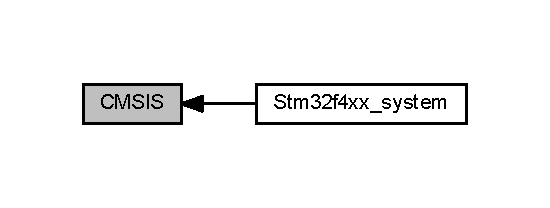
\includegraphics[width=264pt]{group___c_m_s_i_s}
\end{center}
\end{figure}
\subsection*{Modules}
\begin{DoxyCompactItemize}
\item 
\mbox{\hyperlink{group__stm32f4xx__system}{Stm32f4xx\+\_\+system}}
\end{DoxyCompactItemize}


\subsection{Detailed Description}

\hypertarget{group__stm32f4xx__system}{}\section{Stm32f4xx\+\_\+system}
\label{group__stm32f4xx__system}\index{Stm32f4xx\+\_\+system@{Stm32f4xx\+\_\+system}}
Collaboration diagram for Stm32f4xx\+\_\+system\+:
\nopagebreak
\begin{figure}[H]
\begin{center}
\leavevmode
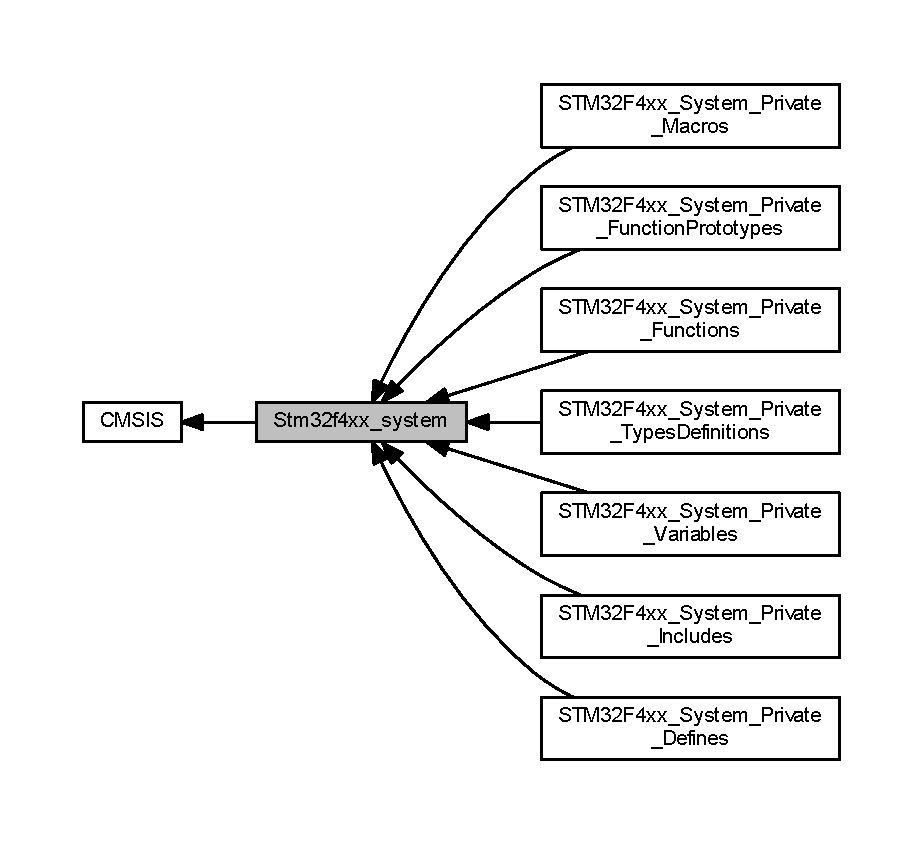
\includegraphics[width=350pt]{group__stm32f4xx__system}
\end{center}
\end{figure}
\subsection*{Modules}
\begin{DoxyCompactItemize}
\item 
\mbox{\hyperlink{group___s_t_m32_f4xx___system___private___includes}{S\+T\+M32\+F4xx\+\_\+\+System\+\_\+\+Private\+\_\+\+Includes}}
\item 
\mbox{\hyperlink{group___s_t_m32_f4xx___system___private___types_definitions}{S\+T\+M32\+F4xx\+\_\+\+System\+\_\+\+Private\+\_\+\+Types\+Definitions}}
\item 
\mbox{\hyperlink{group___s_t_m32_f4xx___system___private___defines}{S\+T\+M32\+F4xx\+\_\+\+System\+\_\+\+Private\+\_\+\+Defines}}
\item 
\mbox{\hyperlink{group___s_t_m32_f4xx___system___private___macros}{S\+T\+M32\+F4xx\+\_\+\+System\+\_\+\+Private\+\_\+\+Macros}}
\item 
\mbox{\hyperlink{group___s_t_m32_f4xx___system___private___variables}{S\+T\+M32\+F4xx\+\_\+\+System\+\_\+\+Private\+\_\+\+Variables}}
\item 
\mbox{\hyperlink{group___s_t_m32_f4xx___system___private___function_prototypes}{S\+T\+M32\+F4xx\+\_\+\+System\+\_\+\+Private\+\_\+\+Function\+Prototypes}}
\item 
\mbox{\hyperlink{group___s_t_m32_f4xx___system___private___functions}{S\+T\+M32\+F4xx\+\_\+\+System\+\_\+\+Private\+\_\+\+Functions}}
\end{DoxyCompactItemize}


\subsection{Detailed Description}

\hypertarget{group___s_t_m32_f4xx___system___private___includes}{}\section{S\+T\+M32\+F4xx\+\_\+\+System\+\_\+\+Private\+\_\+\+Includes}
\label{group___s_t_m32_f4xx___system___private___includes}\index{S\+T\+M32\+F4xx\+\_\+\+System\+\_\+\+Private\+\_\+\+Includes@{S\+T\+M32\+F4xx\+\_\+\+System\+\_\+\+Private\+\_\+\+Includes}}
Collaboration diagram for S\+T\+M32\+F4xx\+\_\+\+System\+\_\+\+Private\+\_\+\+Includes\+:\nopagebreak
\begin{figure}[H]
\begin{center}
\leavevmode
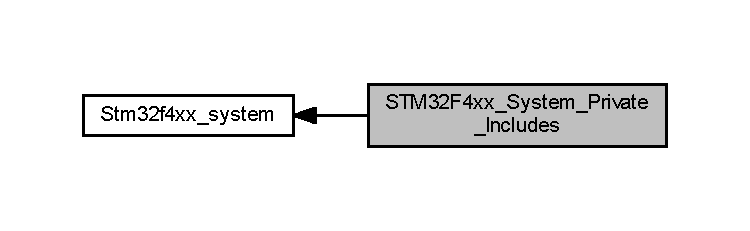
\includegraphics[width=350pt]{group___s_t_m32_f4xx___system___private___includes}
\end{center}
\end{figure}
\subsection*{Macros}
\begin{DoxyCompactItemize}
\item 
\#define \mbox{\hyperlink{group___s_t_m32_f4xx___system___private___includes_gaeafcff4f57440c60e64812dddd13e7cb}{H\+S\+E\+\_\+\+V\+A\+L\+UE}}~((uint32\+\_\+t)25000000)
\item 
\#define \mbox{\hyperlink{group___s_t_m32_f4xx___system___private___includes_gaaa8c76e274d0f6dd2cefb5d0b17fbc37}{H\+S\+I\+\_\+\+V\+A\+L\+UE}}~((uint32\+\_\+t)16000000)
\end{DoxyCompactItemize}


\subsection{Detailed Description}


\subsection{Macro Definition Documentation}
\mbox{\Hypertarget{group___s_t_m32_f4xx___system___private___includes_gaeafcff4f57440c60e64812dddd13e7cb}\label{group___s_t_m32_f4xx___system___private___includes_gaeafcff4f57440c60e64812dddd13e7cb}} 
\index{S\+T\+M32\+F4xx\+\_\+\+System\+\_\+\+Private\+\_\+\+Includes@{S\+T\+M32\+F4xx\+\_\+\+System\+\_\+\+Private\+\_\+\+Includes}!H\+S\+E\+\_\+\+V\+A\+L\+UE@{H\+S\+E\+\_\+\+V\+A\+L\+UE}}
\index{H\+S\+E\+\_\+\+V\+A\+L\+UE@{H\+S\+E\+\_\+\+V\+A\+L\+UE}!S\+T\+M32\+F4xx\+\_\+\+System\+\_\+\+Private\+\_\+\+Includes@{S\+T\+M32\+F4xx\+\_\+\+System\+\_\+\+Private\+\_\+\+Includes}}
\subsubsection{\texorpdfstring{H\+S\+E\+\_\+\+V\+A\+L\+UE}{HSE\_VALUE}}
{\footnotesize\ttfamily \#define H\+S\+E\+\_\+\+V\+A\+L\+UE~((uint32\+\_\+t)25000000)}

Default value of the External oscillator in Hz 

Definition at line 68 of file system\+\_\+stm32f4xx.\+c.

\mbox{\Hypertarget{group___s_t_m32_f4xx___system___private___includes_gaaa8c76e274d0f6dd2cefb5d0b17fbc37}\label{group___s_t_m32_f4xx___system___private___includes_gaaa8c76e274d0f6dd2cefb5d0b17fbc37}} 
\index{S\+T\+M32\+F4xx\+\_\+\+System\+\_\+\+Private\+\_\+\+Includes@{S\+T\+M32\+F4xx\+\_\+\+System\+\_\+\+Private\+\_\+\+Includes}!H\+S\+I\+\_\+\+V\+A\+L\+UE@{H\+S\+I\+\_\+\+V\+A\+L\+UE}}
\index{H\+S\+I\+\_\+\+V\+A\+L\+UE@{H\+S\+I\+\_\+\+V\+A\+L\+UE}!S\+T\+M32\+F4xx\+\_\+\+System\+\_\+\+Private\+\_\+\+Includes@{S\+T\+M32\+F4xx\+\_\+\+System\+\_\+\+Private\+\_\+\+Includes}}
\subsubsection{\texorpdfstring{H\+S\+I\+\_\+\+V\+A\+L\+UE}{HSI\_VALUE}}
{\footnotesize\ttfamily \#define H\+S\+I\+\_\+\+V\+A\+L\+UE~((uint32\+\_\+t)16000000)}

Value of the Internal oscillator in Hz 

Definition at line 72 of file system\+\_\+stm32f4xx.\+c.


\hypertarget{group___s_t_m32_f4xx___system___private___types_definitions}{}\section{S\+T\+M32\+F4xx\+\_\+\+System\+\_\+\+Private\+\_\+\+Types\+Definitions}
\label{group___s_t_m32_f4xx___system___private___types_definitions}\index{S\+T\+M32\+F4xx\+\_\+\+System\+\_\+\+Private\+\_\+\+Types\+Definitions@{S\+T\+M32\+F4xx\+\_\+\+System\+\_\+\+Private\+\_\+\+Types\+Definitions}}
Collaboration diagram for S\+T\+M32\+F4xx\+\_\+\+System\+\_\+\+Private\+\_\+\+Types\+Definitions\+:
\nopagebreak
\begin{figure}[H]
\begin{center}
\leavevmode
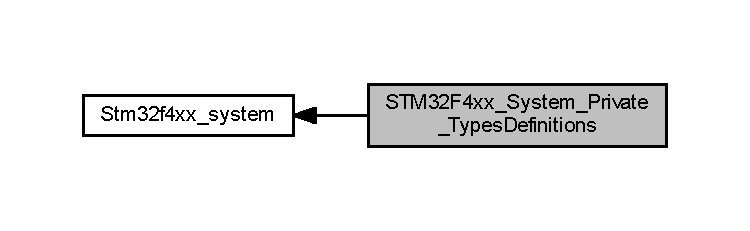
\includegraphics[width=350pt]{group___s_t_m32_f4xx___system___private___types_definitions}
\end{center}
\end{figure}

\hypertarget{group___s_t_m32_f4xx___system___private___defines}{}\section{S\+T\+M32\+F4xx\+\_\+\+System\+\_\+\+Private\+\_\+\+Defines}
\label{group___s_t_m32_f4xx___system___private___defines}\index{S\+T\+M32\+F4xx\+\_\+\+System\+\_\+\+Private\+\_\+\+Defines@{S\+T\+M32\+F4xx\+\_\+\+System\+\_\+\+Private\+\_\+\+Defines}}
Collaboration diagram for S\+T\+M32\+F4xx\+\_\+\+System\+\_\+\+Private\+\_\+\+Defines\+:\nopagebreak
\begin{figure}[H]
\begin{center}
\leavevmode
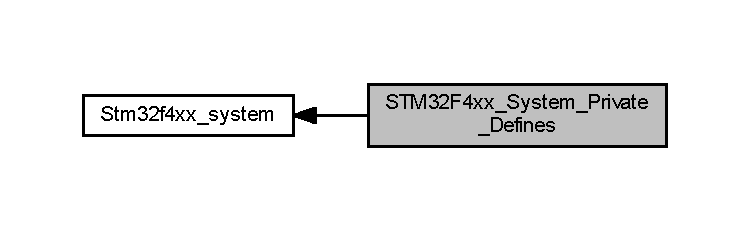
\includegraphics[width=350pt]{group___s_t_m32_f4xx___system___private___defines}
\end{center}
\end{figure}
\subsection*{Macros}
\begin{DoxyCompactItemize}
\item 
\#define \mbox{\hyperlink{group___s_t_m32_f4xx___system___private___defines_ga40e1495541cbb4acbe3f1819bd87a9fe}{V\+E\+C\+T\+\_\+\+T\+A\+B\+\_\+\+O\+F\+F\+S\+ET}}~0x00
\end{DoxyCompactItemize}


\subsection{Detailed Description}


\subsection{Macro Definition Documentation}
\mbox{\Hypertarget{group___s_t_m32_f4xx___system___private___defines_ga40e1495541cbb4acbe3f1819bd87a9fe}\label{group___s_t_m32_f4xx___system___private___defines_ga40e1495541cbb4acbe3f1819bd87a9fe}} 
\index{S\+T\+M32\+F4xx\+\_\+\+System\+\_\+\+Private\+\_\+\+Defines@{S\+T\+M32\+F4xx\+\_\+\+System\+\_\+\+Private\+\_\+\+Defines}!V\+E\+C\+T\+\_\+\+T\+A\+B\+\_\+\+O\+F\+F\+S\+ET@{V\+E\+C\+T\+\_\+\+T\+A\+B\+\_\+\+O\+F\+F\+S\+ET}}
\index{V\+E\+C\+T\+\_\+\+T\+A\+B\+\_\+\+O\+F\+F\+S\+ET@{V\+E\+C\+T\+\_\+\+T\+A\+B\+\_\+\+O\+F\+F\+S\+ET}!S\+T\+M32\+F4xx\+\_\+\+System\+\_\+\+Private\+\_\+\+Defines@{S\+T\+M32\+F4xx\+\_\+\+System\+\_\+\+Private\+\_\+\+Defines}}
\subsubsection{\texorpdfstring{V\+E\+C\+T\+\_\+\+T\+A\+B\+\_\+\+O\+F\+F\+S\+ET}{VECT\_TAB\_OFFSET}}
{\footnotesize\ttfamily \#define V\+E\+C\+T\+\_\+\+T\+A\+B\+\_\+\+O\+F\+F\+S\+ET~0x00}

$<$ Uncomment the following line if you need to use external S\+R\+AM or S\+D\+R\+AM as data memory ~\newline
~\newline
 $<$ Uncomment the following line if you need to relocate your vector \mbox{\hyperlink{struct_table}{Table}} in Internal S\+R\+AM. Vector \mbox{\hyperlink{struct_table}{Table}} base offset field. This value must be a multiple of 0x200. 

Definition at line 109 of file system\+\_\+stm32f4xx.\+c.


\hypertarget{group___s_t_m32_f4xx___system___private___macros}{}\section{S\+T\+M32\+F4xx\+\_\+\+System\+\_\+\+Private\+\_\+\+Macros}
\label{group___s_t_m32_f4xx___system___private___macros}\index{S\+T\+M32\+F4xx\+\_\+\+System\+\_\+\+Private\+\_\+\+Macros@{S\+T\+M32\+F4xx\+\_\+\+System\+\_\+\+Private\+\_\+\+Macros}}
Collaboration diagram for S\+T\+M32\+F4xx\+\_\+\+System\+\_\+\+Private\+\_\+\+Macros\+:\nopagebreak
\begin{figure}[H]
\begin{center}
\leavevmode
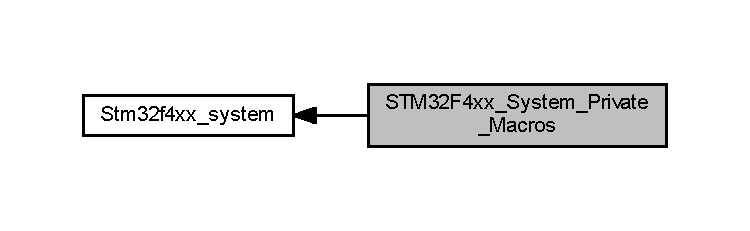
\includegraphics[width=350pt]{group___s_t_m32_f4xx___system___private___macros}
\end{center}
\end{figure}

\hypertarget{group___s_t_m32_f4xx___system___private___variables}{}\section{S\+T\+M32\+F4xx\+\_\+\+System\+\_\+\+Private\+\_\+\+Variables}
\label{group___s_t_m32_f4xx___system___private___variables}\index{S\+T\+M32\+F4xx\+\_\+\+System\+\_\+\+Private\+\_\+\+Variables@{S\+T\+M32\+F4xx\+\_\+\+System\+\_\+\+Private\+\_\+\+Variables}}
Collaboration diagram for S\+T\+M32\+F4xx\+\_\+\+System\+\_\+\+Private\+\_\+\+Variables\+:
\nopagebreak
\begin{figure}[H]
\begin{center}
\leavevmode
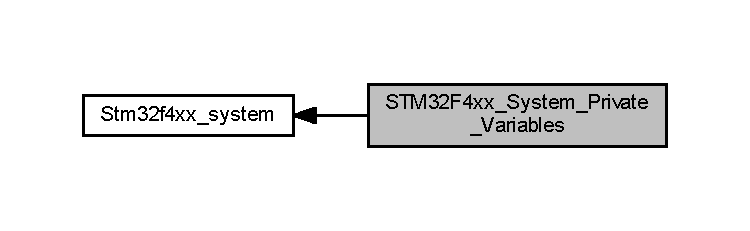
\includegraphics[width=350pt]{group___s_t_m32_f4xx___system___private___variables}
\end{center}
\end{figure}
\subsection*{Variables}
\begin{DoxyCompactItemize}
\item 
uint32\+\_\+t \mbox{\hyperlink{group___s_t_m32_f4xx___system___private___variables_gaa3cd3e43291e81e795d642b79b6088e6}{System\+Core\+Clock}} = 16000000
\item 
const uint8\+\_\+t \mbox{\hyperlink{group___s_t_m32_f4xx___system___private___variables_ga6e1d9cd666f0eacbfde31e9932a93466}{A\+H\+B\+Presc\+Table}} \mbox{[}16\mbox{]} = \{0, 0, 0, 0, 0, 0, 0, 0, 1, 2, 3, 4, 6, 7, 8, 9\}
\item 
const uint8\+\_\+t \mbox{\hyperlink{group___s_t_m32_f4xx___system___private___variables_ga5b4f8b768465842cf854a8f993b375e9}{A\+P\+B\+Presc\+Table}} \mbox{[}8\mbox{]} = \{0, 0, 0, 0, 1, 2, 3, 4\}
\end{DoxyCompactItemize}


\subsection{Detailed Description}


\subsection{Variable Documentation}
\mbox{\Hypertarget{group___s_t_m32_f4xx___system___private___variables_ga6e1d9cd666f0eacbfde31e9932a93466}\label{group___s_t_m32_f4xx___system___private___variables_ga6e1d9cd666f0eacbfde31e9932a93466}} 
\index{S\+T\+M32\+F4xx\+\_\+\+System\+\_\+\+Private\+\_\+\+Variables@{S\+T\+M32\+F4xx\+\_\+\+System\+\_\+\+Private\+\_\+\+Variables}!A\+H\+B\+Presc\+Table@{A\+H\+B\+Presc\+Table}}
\index{A\+H\+B\+Presc\+Table@{A\+H\+B\+Presc\+Table}!S\+T\+M32\+F4xx\+\_\+\+System\+\_\+\+Private\+\_\+\+Variables@{S\+T\+M32\+F4xx\+\_\+\+System\+\_\+\+Private\+\_\+\+Variables}}
\subsubsection{\texorpdfstring{A\+H\+B\+Presc\+Table}{AHBPrescTable}}
{\footnotesize\ttfamily const uint8\+\_\+t A\+H\+B\+Presc\+Table\mbox{[}16\mbox{]} = \{0, 0, 0, 0, 0, 0, 0, 0, 1, 2, 3, 4, 6, 7, 8, 9\}}



Definition at line 138 of file system\+\_\+stm32f4xx.\+c.

\mbox{\Hypertarget{group___s_t_m32_f4xx___system___private___variables_ga5b4f8b768465842cf854a8f993b375e9}\label{group___s_t_m32_f4xx___system___private___variables_ga5b4f8b768465842cf854a8f993b375e9}} 
\index{S\+T\+M32\+F4xx\+\_\+\+System\+\_\+\+Private\+\_\+\+Variables@{S\+T\+M32\+F4xx\+\_\+\+System\+\_\+\+Private\+\_\+\+Variables}!A\+P\+B\+Presc\+Table@{A\+P\+B\+Presc\+Table}}
\index{A\+P\+B\+Presc\+Table@{A\+P\+B\+Presc\+Table}!S\+T\+M32\+F4xx\+\_\+\+System\+\_\+\+Private\+\_\+\+Variables@{S\+T\+M32\+F4xx\+\_\+\+System\+\_\+\+Private\+\_\+\+Variables}}
\subsubsection{\texorpdfstring{A\+P\+B\+Presc\+Table}{APBPrescTable}}
{\footnotesize\ttfamily const uint8\+\_\+t A\+P\+B\+Presc\+Table\mbox{[}8\mbox{]} = \{0, 0, 0, 0, 1, 2, 3, 4\}}



Definition at line 139 of file system\+\_\+stm32f4xx.\+c.

\mbox{\Hypertarget{group___s_t_m32_f4xx___system___private___variables_gaa3cd3e43291e81e795d642b79b6088e6}\label{group___s_t_m32_f4xx___system___private___variables_gaa3cd3e43291e81e795d642b79b6088e6}} 
\index{S\+T\+M32\+F4xx\+\_\+\+System\+\_\+\+Private\+\_\+\+Variables@{S\+T\+M32\+F4xx\+\_\+\+System\+\_\+\+Private\+\_\+\+Variables}!System\+Core\+Clock@{System\+Core\+Clock}}
\index{System\+Core\+Clock@{System\+Core\+Clock}!S\+T\+M32\+F4xx\+\_\+\+System\+\_\+\+Private\+\_\+\+Variables@{S\+T\+M32\+F4xx\+\_\+\+System\+\_\+\+Private\+\_\+\+Variables}}
\subsubsection{\texorpdfstring{System\+Core\+Clock}{SystemCoreClock}}
{\footnotesize\ttfamily uint32\+\_\+t System\+Core\+Clock = 16000000}



Definition at line 137 of file system\+\_\+stm32f4xx.\+c.


\hypertarget{group___s_t_m32_f4xx___system___private___function_prototypes}{}\section{S\+T\+M32\+F4xx\+\_\+\+System\+\_\+\+Private\+\_\+\+Function\+Prototypes}
\label{group___s_t_m32_f4xx___system___private___function_prototypes}\index{S\+T\+M32\+F4xx\+\_\+\+System\+\_\+\+Private\+\_\+\+Function\+Prototypes@{S\+T\+M32\+F4xx\+\_\+\+System\+\_\+\+Private\+\_\+\+Function\+Prototypes}}
Collaboration diagram for S\+T\+M32\+F4xx\+\_\+\+System\+\_\+\+Private\+\_\+\+Function\+Prototypes\+:
\nopagebreak
\begin{figure}[H]
\begin{center}
\leavevmode
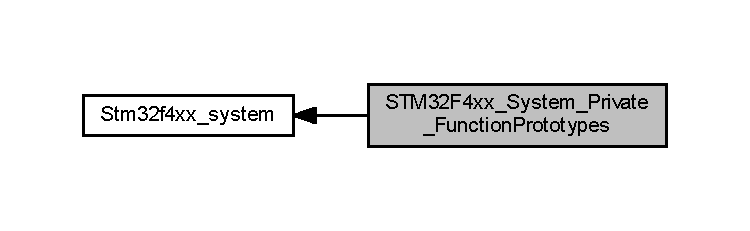
\includegraphics[width=350pt]{group___s_t_m32_f4xx___system___private___function_prototypes}
\end{center}
\end{figure}

\hypertarget{group___s_t_m32_f4xx___system___private___functions}{}\section{S\+T\+M32\+F4xx\+\_\+\+System\+\_\+\+Private\+\_\+\+Functions}
\label{group___s_t_m32_f4xx___system___private___functions}\index{S\+T\+M32\+F4xx\+\_\+\+System\+\_\+\+Private\+\_\+\+Functions@{S\+T\+M32\+F4xx\+\_\+\+System\+\_\+\+Private\+\_\+\+Functions}}
Collaboration diagram for S\+T\+M32\+F4xx\+\_\+\+System\+\_\+\+Private\+\_\+\+Functions\+:\nopagebreak
\begin{figure}[H]
\begin{center}
\leavevmode
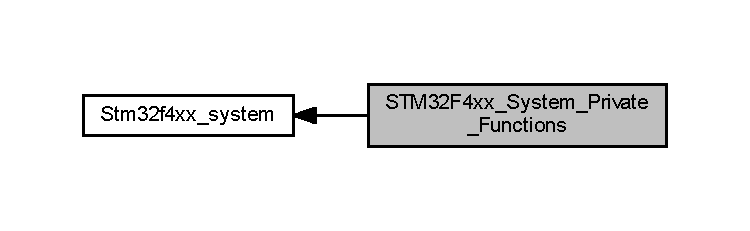
\includegraphics[width=350pt]{group___s_t_m32_f4xx___system___private___functions}
\end{center}
\end{figure}
\subsection*{Functions}
\begin{DoxyCompactItemize}
\item 
void \mbox{\hyperlink{group___s_t_m32_f4xx___system___private___functions_ga93f514700ccf00d08dbdcff7f1224eb2}{System\+Init}} (void)
\begin{DoxyCompactList}\small\item\em Setup the microcontroller system Initialize the F\+PU setting, vector table location and External memory configuration. \end{DoxyCompactList}\item 
void \mbox{\hyperlink{group___s_t_m32_f4xx___system___private___functions_gae0c36a9591fe6e9c45ecb21a794f0f0f}{System\+Core\+Clock\+Update}} (void)
\begin{DoxyCompactList}\small\item\em Update System\+Core\+Clock variable according to Clock Register Values. The System\+Core\+Clock variable contains the core clock (H\+C\+LK), it can be used by the user application to setup the Sys\+Tick timer or configure other parameters. \end{DoxyCompactList}\end{DoxyCompactItemize}


\subsection{Detailed Description}


\subsection{Function Documentation}
\mbox{\Hypertarget{group___s_t_m32_f4xx___system___private___functions_gae0c36a9591fe6e9c45ecb21a794f0f0f}\label{group___s_t_m32_f4xx___system___private___functions_gae0c36a9591fe6e9c45ecb21a794f0f0f}} 
\index{S\+T\+M32\+F4xx\+\_\+\+System\+\_\+\+Private\+\_\+\+Functions@{S\+T\+M32\+F4xx\+\_\+\+System\+\_\+\+Private\+\_\+\+Functions}!System\+Core\+Clock\+Update@{System\+Core\+Clock\+Update}}
\index{System\+Core\+Clock\+Update@{System\+Core\+Clock\+Update}!S\+T\+M32\+F4xx\+\_\+\+System\+\_\+\+Private\+\_\+\+Functions@{S\+T\+M32\+F4xx\+\_\+\+System\+\_\+\+Private\+\_\+\+Functions}}
\subsubsection{\texorpdfstring{System\+Core\+Clock\+Update()}{SystemCoreClockUpdate()}}
{\footnotesize\ttfamily void System\+Core\+Clock\+Update (\begin{DoxyParamCaption}\item[{void}]{ }\end{DoxyParamCaption})}



Update System\+Core\+Clock variable according to Clock Register Values. The System\+Core\+Clock variable contains the core clock (H\+C\+LK), it can be used by the user application to setup the Sys\+Tick timer or configure other parameters. 

\begin{DoxyNote}{Note}
Each time the core clock (H\+C\+LK) changes, this function must be called to update System\+Core\+Clock variable value. Otherwise, any configuration based on this variable will be incorrect. ~\newline
 

-\/ The system frequency computed by this function is not the real frequency in the chip. It is calculated based on the predefined constant and the selected clock source\+:
\end{DoxyNote}

\begin{DoxyItemize}
\item If S\+Y\+S\+C\+LK source is H\+SI, System\+Core\+Clock will contain the \mbox{\hyperlink{group___s_t_m32_f4xx___system___private___includes_gaaa8c76e274d0f6dd2cefb5d0b17fbc37}{H\+S\+I\+\_\+\+V\+A\+L\+U\+E($\ast$)}}
\item If S\+Y\+S\+C\+LK source is H\+SE, System\+Core\+Clock will contain the \mbox{\hyperlink{group___s_t_m32_f4xx___system___private___includes_gaeafcff4f57440c60e64812dddd13e7cb}{H\+S\+E\+\_\+\+V\+A\+L\+U\+E($\ast$$\ast$)}}
\item If S\+Y\+S\+C\+LK source is P\+LL, System\+Core\+Clock will contain the \mbox{\hyperlink{group___s_t_m32_f4xx___system___private___includes_gaeafcff4f57440c60e64812dddd13e7cb}{H\+S\+E\+\_\+\+V\+A\+L\+U\+E($\ast$$\ast$)}} or \mbox{\hyperlink{group___s_t_m32_f4xx___system___private___includes_gaaa8c76e274d0f6dd2cefb5d0b17fbc37}{H\+S\+I\+\_\+\+V\+A\+L\+U\+E($\ast$)}} multiplied/divided by the P\+LL factors.
\end{DoxyItemize}

($\ast$) H\+S\+I\+\_\+\+V\+A\+L\+UE is a constant defined in \mbox{\hyperlink{stm32f4xx__hal__conf_8h}{stm32f4xx\+\_\+hal\+\_\+conf.\+h}} file (default value 16 M\+Hz) but the real value may vary depending on the variations in voltage and temperature. ~\newline
 ($\ast$$\ast$) H\+S\+E\+\_\+\+V\+A\+L\+UE is a constant defined in \mbox{\hyperlink{stm32f4xx__hal__conf_8h}{stm32f4xx\+\_\+hal\+\_\+conf.\+h}} file (its value depends on the application requirements), user has to ensure that H\+S\+E\+\_\+\+V\+A\+L\+UE is same as the real frequency of the crystal used. Otherwise, this function may have wrong result.


\begin{DoxyItemize}
\item The result of this function could be not correct when using fractional value for H\+SE crystal.
\end{DoxyItemize}


\begin{DoxyParams}{Parameters}
{\em None} & \\
\hline
\end{DoxyParams}

\begin{DoxyRetVals}{Return values}
{\em None} & \\
\hline
\end{DoxyRetVals}


Definition at line 240 of file system\+\_\+stm32f4xx.\+c.

\mbox{\Hypertarget{group___s_t_m32_f4xx___system___private___functions_ga93f514700ccf00d08dbdcff7f1224eb2}\label{group___s_t_m32_f4xx___system___private___functions_ga93f514700ccf00d08dbdcff7f1224eb2}} 
\index{S\+T\+M32\+F4xx\+\_\+\+System\+\_\+\+Private\+\_\+\+Functions@{S\+T\+M32\+F4xx\+\_\+\+System\+\_\+\+Private\+\_\+\+Functions}!System\+Init@{System\+Init}}
\index{System\+Init@{System\+Init}!S\+T\+M32\+F4xx\+\_\+\+System\+\_\+\+Private\+\_\+\+Functions@{S\+T\+M32\+F4xx\+\_\+\+System\+\_\+\+Private\+\_\+\+Functions}}
\subsubsection{\texorpdfstring{System\+Init()}{SystemInit()}}
{\footnotesize\ttfamily void System\+Init (\begin{DoxyParamCaption}\item[{void}]{ }\end{DoxyParamCaption})}



Setup the microcontroller system Initialize the F\+PU setting, vector table location and External memory configuration. 


\begin{DoxyParams}{Parameters}
{\em None} & \\
\hline
\end{DoxyParams}

\begin{DoxyRetVals}{Return values}
{\em None} & \\
\hline
\end{DoxyRetVals}


Definition at line 167 of file system\+\_\+stm32f4xx.\+c.


\chapter{Data Structure Documentation}
\hypertarget{union_column_buffer__}{}\section{Column\+Buffer\+\_\+ Union Reference}
\label{union_column_buffer__}\index{Column\+Buffer\+\_\+@{Column\+Buffer\+\_\+}}
\subsection*{Data Fields}
\begin{DoxyCompactItemize}
\item 
uint32\+\_\+t \mbox{\hyperlink{union_column_buffer___a582fa2ca99b13c0df79f2fd2445ac31e}{raw\+Data}}
\item 
page\+Set \mbox{\hyperlink{union_column_buffer___a7e95b3d635528dfbaee7b3ea7b305277}{page\+Set}}
\end{DoxyCompactItemize}


\subsection{Detailed Description}


Definition at line 82 of file lcd\+\_\+driver.\+c.



\subsection{Field Documentation}
\mbox{\Hypertarget{union_column_buffer___a7e95b3d635528dfbaee7b3ea7b305277}\label{union_column_buffer___a7e95b3d635528dfbaee7b3ea7b305277}} 
\index{Column\+Buffer\+\_\+@{Column\+Buffer\+\_\+}!page\+Set@{page\+Set}}
\index{page\+Set@{page\+Set}!Column\+Buffer\+\_\+@{Column\+Buffer\+\_\+}}
\subsubsection{\texorpdfstring{page\+Set}{pageSet}}
{\footnotesize\ttfamily page\+Set page\+Set}



Definition at line 84 of file lcd\+\_\+driver.\+c.

\mbox{\Hypertarget{union_column_buffer___a582fa2ca99b13c0df79f2fd2445ac31e}\label{union_column_buffer___a582fa2ca99b13c0df79f2fd2445ac31e}} 
\index{Column\+Buffer\+\_\+@{Column\+Buffer\+\_\+}!raw\+Data@{raw\+Data}}
\index{raw\+Data@{raw\+Data}!Column\+Buffer\+\_\+@{Column\+Buffer\+\_\+}}
\subsubsection{\texorpdfstring{raw\+Data}{rawData}}
{\footnotesize\ttfamily uint32\+\_\+t raw\+Data}



Definition at line 83 of file lcd\+\_\+driver.\+c.



The documentation for this union was generated from the following file\+:\begin{DoxyCompactItemize}
\item 
Library/\+Library/src/\mbox{\hyperlink{lcd__driver_8c}{lcd\+\_\+driver.\+c}}\end{DoxyCompactItemize}

\hypertarget{struct_font_size__}{}\section{Font\+Size\+\_\+ Struct Reference}
\label{struct_font_size__}\index{Font\+Size\+\_\+@{Font\+Size\+\_\+}}
\subsection*{Data Fields}
\begin{DoxyCompactItemize}
\item 
uint8\+\_\+t \mbox{\hyperlink{struct_font_size___adcf201a8aabf55cb352ec05331242594}{height}}
\item 
uint8\+\_\+t \mbox{\hyperlink{struct_font_size___a09a2a45f731b02946ff6d3cd15c1a476}{width}}
\end{DoxyCompactItemize}


\subsection{Detailed Description}


Definition at line 71 of file lcd\+\_\+driver.\+c.



\subsection{Field Documentation}
\mbox{\Hypertarget{struct_font_size___adcf201a8aabf55cb352ec05331242594}\label{struct_font_size___adcf201a8aabf55cb352ec05331242594}} 
\index{Font\+Size\+\_\+@{Font\+Size\+\_\+}!height@{height}}
\index{height@{height}!Font\+Size\+\_\+@{Font\+Size\+\_\+}}
\subsubsection{\texorpdfstring{height}{height}}
{\footnotesize\ttfamily uint8\+\_\+t height}



Definition at line 72 of file lcd\+\_\+driver.\+c.

\mbox{\Hypertarget{struct_font_size___a09a2a45f731b02946ff6d3cd15c1a476}\label{struct_font_size___a09a2a45f731b02946ff6d3cd15c1a476}} 
\index{Font\+Size\+\_\+@{Font\+Size\+\_\+}!width@{width}}
\index{width@{width}!Font\+Size\+\_\+@{Font\+Size\+\_\+}}
\subsubsection{\texorpdfstring{width}{width}}
{\footnotesize\ttfamily uint8\+\_\+t width}



Definition at line 73 of file lcd\+\_\+driver.\+c.



The documentation for this struct was generated from the following file\+:\begin{DoxyCompactItemize}
\item 
Src/\mbox{\hyperlink{lcd__driver_8c}{lcd\+\_\+driver.\+c}}\end{DoxyCompactItemize}

\chapter{File Documentation}
\hypertarget{button_8c}{}\section{Library/\+Library/src/button.c File Reference}
\label{button_8c}\index{Library/\+Library/src/button.\+c@{Library/\+Library/src/button.\+c}}
{\ttfamily \#include \char`\"{}button.\+h\char`\"{}}\newline
{\ttfamily \#include \char`\"{}button\+\_\+driver.\+h\char`\"{}}\newline
Include dependency graph for button.\+c\+:\nopagebreak
\begin{figure}[H]
\begin{center}
\leavevmode
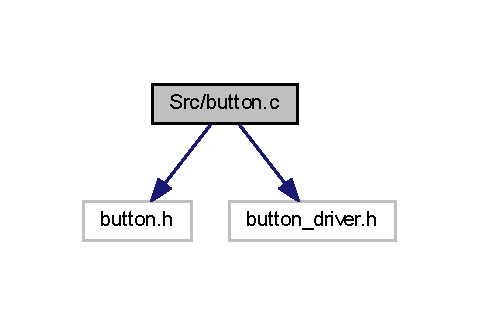
\includegraphics[width=350pt]{button_8c__incl}
\end{center}
\end{figure}
\subsection*{Macros}
\begin{DoxyCompactItemize}
\item 
\#define \mbox{\hyperlink{button_8c_ae0ff96edce0aa2def3ba1e6b56564e00}{M\+A\+X\+\_\+\+N\+U\+M\+B\+E\+R\+\_\+\+O\+F\+\_\+\+F\+I\+L\+T\+E\+RS}}~10
\end{DoxyCompactItemize}
\subsection*{Functions}
\begin{DoxyCompactItemize}
\item 
uint8\+\_\+t \mbox{\hyperlink{button_8c_af2c0ff777b822ad89ae3df68ca0c5e4b}{Button\+\_\+init}} (\mbox{\hyperlink{button_8h_ab369ab7fa0b9a8dfec4fc1f653ac6de5}{Button}} $\ast$const \+\_\+this, G\+P\+I\+O\+\_\+\+Type\+Def $\ast$const port, uint16\+\_\+t pin)
\end{DoxyCompactItemize}


\subsection{Macro Definition Documentation}
\mbox{\Hypertarget{button_8c_ae0ff96edce0aa2def3ba1e6b56564e00}\label{button_8c_ae0ff96edce0aa2def3ba1e6b56564e00}} 
\index{button.\+c@{button.\+c}!M\+A\+X\+\_\+\+N\+U\+M\+B\+E\+R\+\_\+\+O\+F\+\_\+\+F\+I\+L\+T\+E\+RS@{M\+A\+X\+\_\+\+N\+U\+M\+B\+E\+R\+\_\+\+O\+F\+\_\+\+F\+I\+L\+T\+E\+RS}}
\index{M\+A\+X\+\_\+\+N\+U\+M\+B\+E\+R\+\_\+\+O\+F\+\_\+\+F\+I\+L\+T\+E\+RS@{M\+A\+X\+\_\+\+N\+U\+M\+B\+E\+R\+\_\+\+O\+F\+\_\+\+F\+I\+L\+T\+E\+RS}!button.\+c@{button.\+c}}
\subsubsection{\texorpdfstring{M\+A\+X\+\_\+\+N\+U\+M\+B\+E\+R\+\_\+\+O\+F\+\_\+\+F\+I\+L\+T\+E\+RS}{MAX\_NUMBER\_OF\_FILTERS}}
{\footnotesize\ttfamily \#define M\+A\+X\+\_\+\+N\+U\+M\+B\+E\+R\+\_\+\+O\+F\+\_\+\+F\+I\+L\+T\+E\+RS~10}



Definition at line 5 of file button.\+c.



\subsection{Function Documentation}
\mbox{\Hypertarget{button_8c_af2c0ff777b822ad89ae3df68ca0c5e4b}\label{button_8c_af2c0ff777b822ad89ae3df68ca0c5e4b}} 
\index{button.\+c@{button.\+c}!Button\+\_\+init@{Button\+\_\+init}}
\index{Button\+\_\+init@{Button\+\_\+init}!button.\+c@{button.\+c}}
\subsubsection{\texorpdfstring{Button\+\_\+init()}{Button\_init()}}
{\footnotesize\ttfamily uint8\+\_\+t Button\+\_\+init (\begin{DoxyParamCaption}\item[{\mbox{\hyperlink{button_8h_ab369ab7fa0b9a8dfec4fc1f653ac6de5}{Button}} $\ast$const}]{\+\_\+this,  }\item[{G\+P\+I\+O\+\_\+\+Type\+Def $\ast$const}]{port,  }\item[{uint16\+\_\+t}]{pin }\end{DoxyParamCaption})}



Definition at line 20 of file button.\+c.

Here is the caller graph for this function\+:\nopagebreak
\begin{figure}[H]
\begin{center}
\leavevmode
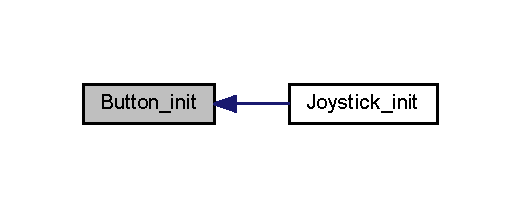
\includegraphics[width=324pt]{button_8c_af2c0ff777b822ad89ae3df68ca0c5e4b_icgraph}
\end{center}
\end{figure}

\hypertarget{button__driver_8c}{}\section{Src/button\+\_\+driver.c File Reference}
\label{button__driver_8c}\index{Src/button\+\_\+driver.\+c@{Src/button\+\_\+driver.\+c}}
{\ttfamily \#include \char`\"{}button\+\_\+driver.\+h\char`\"{}}\newline
Include dependency graph for button\+\_\+driver.\+c\+:\nopagebreak
\begin{figure}[H]
\begin{center}
\leavevmode
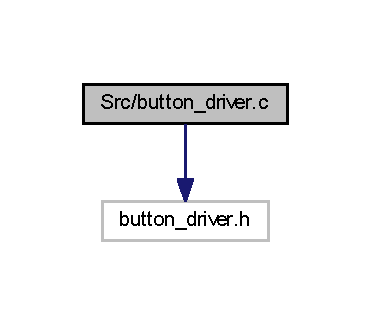
\includegraphics[width=178pt]{button__driver_8c__incl}
\end{center}
\end{figure}
\subsection*{Functions}
\begin{DoxyCompactItemize}
\item 
uint8\+\_\+t \mbox{\hyperlink{button__driver_8c_a61dbff7d557fc276d145eddf49b0bbe1}{Input\+Filter\+\_\+init}} (Input\+Filter $\ast$const \+\_\+this, G\+P\+I\+O\+\_\+\+Type\+Def $\ast$const port, uint16\+\_\+t pin)
\end{DoxyCompactItemize}


\subsection{Function Documentation}
\mbox{\Hypertarget{button__driver_8c_a61dbff7d557fc276d145eddf49b0bbe1}\label{button__driver_8c_a61dbff7d557fc276d145eddf49b0bbe1}} 
\index{button\+\_\+driver.\+c@{button\+\_\+driver.\+c}!Input\+Filter\+\_\+init@{Input\+Filter\+\_\+init}}
\index{Input\+Filter\+\_\+init@{Input\+Filter\+\_\+init}!button\+\_\+driver.\+c@{button\+\_\+driver.\+c}}
\subsubsection{\texorpdfstring{Input\+Filter\+\_\+init()}{InputFilter\_init()}}
{\footnotesize\ttfamily uint8\+\_\+t Input\+Filter\+\_\+init (\begin{DoxyParamCaption}\item[{Input\+Filter $\ast$const}]{\+\_\+this,  }\item[{G\+P\+I\+O\+\_\+\+Type\+Def $\ast$const}]{port,  }\item[{uint16\+\_\+t}]{pin }\end{DoxyParamCaption})}



Definition at line 33 of file button\+\_\+driver.\+c.


\hypertarget{gpio_8c}{}\section{Src/gpio.c File Reference}
\label{gpio_8c}\index{Src/gpio.\+c@{Src/gpio.\+c}}
{\ttfamily \#include \char`\"{}gpio.\+h\char`\"{}}\newline
Include dependency graph for gpio.\+c\+:\nopagebreak
\begin{figure}[H]
\begin{center}
\leavevmode
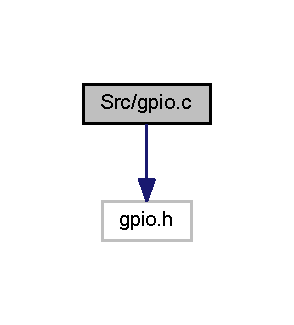
\includegraphics[width=173pt]{gpio_8c__incl}
\end{center}
\end{figure}
\subsection*{Functions}
\begin{DoxyCompactItemize}
\item 
void \mbox{\hyperlink{gpio_8c_ac724e431d2af879252de35615be2bdea}{M\+X\+\_\+\+G\+P\+I\+O\+\_\+\+Init}} (void)
\end{DoxyCompactItemize}


\subsection{Function Documentation}
\mbox{\Hypertarget{gpio_8c_ac724e431d2af879252de35615be2bdea}\label{gpio_8c_ac724e431d2af879252de35615be2bdea}} 
\index{gpio.\+c@{gpio.\+c}!M\+X\+\_\+\+G\+P\+I\+O\+\_\+\+Init@{M\+X\+\_\+\+G\+P\+I\+O\+\_\+\+Init}}
\index{M\+X\+\_\+\+G\+P\+I\+O\+\_\+\+Init@{M\+X\+\_\+\+G\+P\+I\+O\+\_\+\+Init}!gpio.\+c@{gpio.\+c}}
\subsubsection{\texorpdfstring{M\+X\+\_\+\+G\+P\+I\+O\+\_\+\+Init()}{MX\_GPIO\_Init()}}
{\footnotesize\ttfamily void M\+X\+\_\+\+G\+P\+I\+O\+\_\+\+Init (\begin{DoxyParamCaption}\item[{void}]{ }\end{DoxyParamCaption})}

File Name \+: \mbox{\hyperlink{gpio_8c}{gpio.\+c}} Description \+: This file provides code for the configuration of all used G\+P\+IO pins.

This notice applies to any and all portions of this file that are not between comment pairs U\+S\+ER C\+O\+DE B\+E\+G\+IN and U\+S\+ER C\+O\+DE E\+ND. Other portions of this file, whether inserted by the user or by software development tools are owned by their respective copyright owners.

Copyright (c) 2018 S\+T\+Microelectronics International N.\+V. All rights reserved.

Redistribution and use in source and binary forms, with or without modification, are permitted, provided that the following conditions are met\+:


\begin{DoxyEnumerate}
\item Redistribution of source code must retain the above copyright notice, this list of conditions and the following disclaimer.
\item Redistributions in binary form must reproduce the above copyright notice, this list of conditions and the following disclaimer in the documentation and/or other materials provided with the distribution.
\item Neither the name of S\+T\+Microelectronics nor the names of other contributors to this software may be used to endorse or promote products derived from this software without specific written permission.
\item This software, including modifications and/or derivative works of this software, must execute solely and exclusively on microcontroller or microprocessor devices manufactured by or for S\+T\+Microelectronics.
\item Redistribution and use of this software other than as permitted under this license is void and will automatically terminate your rights under this license.
\end{DoxyEnumerate}

T\+H\+IS S\+O\+F\+T\+W\+A\+RE IS P\+R\+O\+V\+I\+D\+ED BY S\+T\+M\+I\+C\+R\+O\+E\+L\+E\+C\+T\+R\+O\+N\+I\+CS A\+ND C\+O\+N\+T\+R\+I\+B\+U\+T\+O\+RS \char`\"{}\+A\+S I\+S\char`\"{} A\+ND A\+NY E\+X\+P\+R\+E\+SS, I\+M\+P\+L\+I\+ED OR S\+T\+A\+T\+U\+T\+O\+RY W\+A\+R\+R\+A\+N\+T\+I\+ES, I\+N\+C\+L\+U\+D\+I\+NG, B\+UT N\+OT L\+I\+M\+I\+T\+ED TO, T\+HE I\+M\+P\+L\+I\+ED W\+A\+R\+R\+A\+N\+T\+I\+ES OF M\+E\+R\+C\+H\+A\+N\+T\+A\+B\+I\+L\+I\+TY, F\+I\+T\+N\+E\+SS F\+OR A P\+A\+R\+T\+I\+C\+U\+L\+AR P\+U\+R\+P\+O\+SE A\+ND N\+O\+N-\/\+I\+N\+F\+R\+I\+N\+G\+E\+M\+E\+NT OF T\+H\+I\+RD P\+A\+R\+TY I\+N\+T\+E\+L\+L\+E\+C\+T\+U\+AL P\+R\+O\+P\+E\+R\+TY R\+I\+G\+H\+TS A\+RE D\+I\+S\+C\+L\+A\+I\+M\+ED TO T\+HE F\+U\+L\+L\+E\+ST E\+X\+T\+E\+NT P\+E\+R\+M\+I\+T\+T\+ED BY L\+AW. IN NO E\+V\+E\+NT S\+H\+A\+LL S\+T\+M\+I\+C\+R\+O\+E\+L\+E\+C\+T\+R\+O\+N\+I\+CS OR C\+O\+N\+T\+R\+I\+B\+U\+T\+O\+RS BE L\+I\+A\+B\+LE F\+OR A\+NY D\+I\+R\+E\+CT, I\+N\+D\+I\+R\+E\+CT, I\+N\+C\+I\+D\+E\+N\+T\+AL, S\+P\+E\+C\+I\+AL, E\+X\+E\+M\+P\+L\+A\+RY, OR C\+O\+N\+S\+E\+Q\+U\+E\+N\+T\+I\+AL D\+A\+M\+A\+G\+ES (I\+N\+C\+L\+U\+D\+I\+NG, B\+UT N\+OT L\+I\+M\+I\+T\+ED TO, P\+R\+O\+C\+U\+R\+E\+M\+E\+NT OF S\+U\+B\+S\+T\+I\+T\+U\+TE G\+O\+O\+DS OR S\+E\+R\+V\+I\+C\+ES; L\+O\+SS OF U\+SE, D\+A\+TA, OR P\+R\+O\+F\+I\+TS; OR B\+U\+S\+I\+N\+E\+SS I\+N\+T\+E\+R\+R\+U\+P\+T\+I\+ON) H\+O\+W\+E\+V\+ER C\+A\+U\+S\+ED A\+ND ON A\+NY T\+H\+E\+O\+RY OF L\+I\+A\+B\+I\+L\+I\+TY, W\+H\+E\+T\+H\+ER IN C\+O\+N\+T\+R\+A\+CT, S\+T\+R\+I\+CT L\+I\+A\+B\+I\+L\+I\+TY, OR T\+O\+RT (I\+N\+C\+L\+U\+D\+I\+NG N\+E\+G\+L\+I\+G\+E\+N\+CE OR O\+T\+H\+E\+R\+W\+I\+SE) A\+R\+I\+S\+I\+NG IN A\+NY W\+AY O\+UT OF T\+HE U\+SE OF T\+H\+IS S\+O\+F\+T\+W\+A\+RE, E\+V\+EN IF A\+D\+V\+I\+S\+ED OF T\+HE P\+O\+S\+S\+I\+B\+I\+L\+I\+TY OF S\+U\+CH D\+A\+M\+A\+G\+E.\+Configure pins as Analog Input Output E\+V\+E\+N\+T\+\_\+\+O\+UT E\+X\+TI 

Definition at line 70 of file gpio.\+c.

Here is the caller graph for this function\+:\nopagebreak
\begin{figure}[H]
\begin{center}
\leavevmode
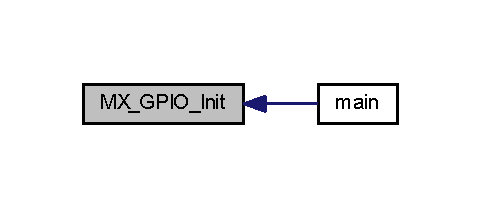
\includegraphics[width=231pt]{gpio_8c_ac724e431d2af879252de35615be2bdea_icgraph}
\end{center}
\end{figure}

\hypertarget{joystick_8c}{}\section{Src/joystick.c File Reference}
\label{joystick_8c}\index{Src/joystick.\+c@{Src/joystick.\+c}}
{\ttfamily \#include \char`\"{}joystick.\+h\char`\"{}}\newline
Include dependency graph for joystick.\+c\+:\nopagebreak
\begin{figure}[H]
\begin{center}
\leavevmode
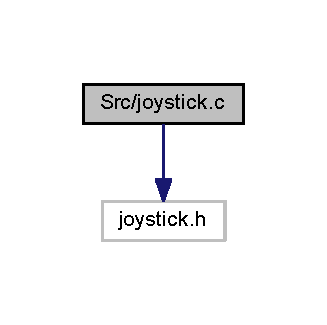
\includegraphics[width=157pt]{joystick_8c__incl}
\end{center}
\end{figure}
\subsection*{Functions}
\begin{DoxyCompactItemize}
\item 
joystick\+Direction \mbox{\hyperlink{joystick_8c_ac2e3ec45ed738f30b06b5417aead9d20}{Joystick\+\_\+get\+Direction}} (Joystick $\ast$const \+\_\+this)
\item 
uint8\+\_\+t \mbox{\hyperlink{joystick_8c_a4aba3c14890c4eaddd13e36b9e782ba4}{Joystick\+\_\+init}} (Joystick $\ast$const \+\_\+this)
\end{DoxyCompactItemize}


\subsection{Function Documentation}
\mbox{\Hypertarget{joystick_8c_ac2e3ec45ed738f30b06b5417aead9d20}\label{joystick_8c_ac2e3ec45ed738f30b06b5417aead9d20}} 
\index{joystick.\+c@{joystick.\+c}!Joystick\+\_\+get\+Direction@{Joystick\+\_\+get\+Direction}}
\index{Joystick\+\_\+get\+Direction@{Joystick\+\_\+get\+Direction}!joystick.\+c@{joystick.\+c}}
\subsubsection{\texorpdfstring{Joystick\+\_\+get\+Direction()}{Joystick\_getDirection()}}
{\footnotesize\ttfamily joystick\+Direction Joystick\+\_\+get\+Direction (\begin{DoxyParamCaption}\item[{Joystick $\ast$const}]{\+\_\+this }\end{DoxyParamCaption})}



Definition at line 16 of file joystick.\+c.

\mbox{\Hypertarget{joystick_8c_a4aba3c14890c4eaddd13e36b9e782ba4}\label{joystick_8c_a4aba3c14890c4eaddd13e36b9e782ba4}} 
\index{joystick.\+c@{joystick.\+c}!Joystick\+\_\+init@{Joystick\+\_\+init}}
\index{Joystick\+\_\+init@{Joystick\+\_\+init}!joystick.\+c@{joystick.\+c}}
\subsubsection{\texorpdfstring{Joystick\+\_\+init()}{Joystick\_init()}}
{\footnotesize\ttfamily uint8\+\_\+t Joystick\+\_\+init (\begin{DoxyParamCaption}\item[{Joystick $\ast$const}]{\+\_\+this }\end{DoxyParamCaption})}



Definition at line 29 of file joystick.\+c.

Here is the call graph for this function\+:\nopagebreak
\begin{figure}[H]
\begin{center}
\leavevmode
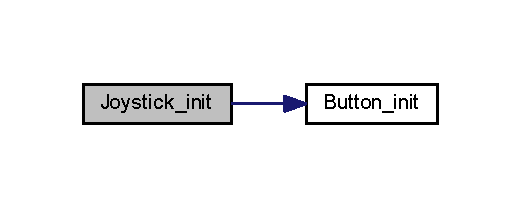
\includegraphics[width=250pt]{joystick_8c_a4aba3c14890c4eaddd13e36b9e782ba4_cgraph}
\end{center}
\end{figure}

\hypertarget{lcd__driver_8c}{}\section{Library/\+Library/src/lcd\+\_\+driver.c File Reference}
\label{lcd__driver_8c}\index{Library/\+Library/src/lcd\+\_\+driver.\+c@{Library/\+Library/src/lcd\+\_\+driver.\+c}}
{\ttfamily \#include \char`\"{}lcd\+\_\+driver.\+h\char`\"{}}\newline
{\ttfamily \#include \char`\"{}lcd\+\_\+symbols.\+h\char`\"{}}\newline
{\ttfamily \#include \char`\"{}lcd\+\_\+font6x8.\+h\char`\"{}}\newline
{\ttfamily \#include \char`\"{}lcd\+\_\+font16x24.\+h\char`\"{}}\newline
{\ttfamily \#include \char`\"{}stm32f4xx\+\_\+hal.\+h\char`\"{}}\newline
{\ttfamily \#include \char`\"{}spi.\+h\char`\"{}}\newline
{\ttfamily \#include $<$stdlib.\+h$>$}\newline
{\ttfamily \#include $<$string.\+h$>$}\newline
{\ttfamily \#include $<$stdbool.\+h$>$}\newline
Include dependency graph for lcd\+\_\+driver.\+c\+:\nopagebreak
\begin{figure}[H]
\begin{center}
\leavevmode
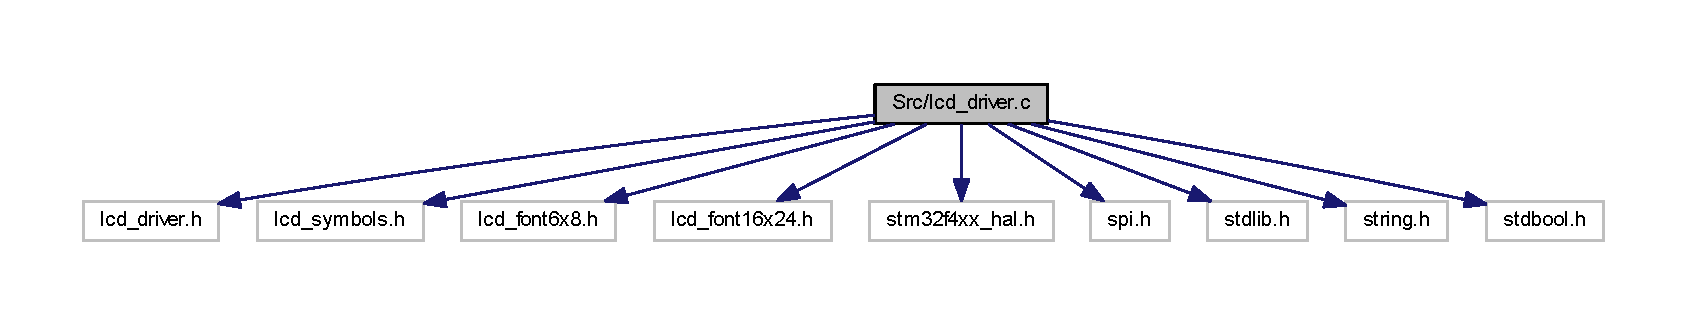
\includegraphics[width=350pt]{lcd__driver_8c__incl}
\end{center}
\end{figure}
\subsection*{Data Structures}
\begin{DoxyCompactItemize}
\item 
struct \mbox{\hyperlink{struct_font_size__}{Font\+Size\+\_\+}}
\item 
union \mbox{\hyperlink{union_column_buffer__}{Column\+Buffer\+\_\+}}
\end{DoxyCompactItemize}
\subsection*{Macros}
\begin{DoxyCompactItemize}
\item 
\#define \mbox{\hyperlink{lcd__driver_8c_a00ad6a3a94ffdd1bc6b55e789f9dfda9}{N\+U\+M\+B\+E\+R\+\_\+\+O\+F\+\_\+\+R\+O\+WS}}~((uint8\+\_\+t) 128)
\item 
\#define \mbox{\hyperlink{lcd__driver_8c_a0240364487a54a70da4ffb51459ada98}{N\+U\+M\+B\+E\+R\+\_\+\+O\+F\+\_\+\+C\+O\+L\+U\+M\+NS}}~((uint8\+\_\+t) 32)
\item 
\#define \mbox{\hyperlink{lcd__driver_8c_a66dfd8dedf4b17144f36e139cce0d1ad}{E\+L\+E\+C\+T\+R\+O\+N\+I\+C\+\_\+\+V\+O\+L\+U\+M\+E\+\_\+\+M\+A\+X\+I\+M\+U\+M\+\_\+\+R\+A\+I\+T\+I\+NG}}~((uint8\+\_\+t) 63)
\item 
\#define \mbox{\hyperlink{lcd__driver_8c_a558990598d0f9a2251ad7ffdb285150a}{A\+S\+C\+I\+I\+\_\+\+T\+A\+B\+L\+E\+\_\+\+O\+F\+F\+S\+ET}}~((uint8\+\_\+t) 32)
\end{DoxyCompactItemize}
\subsection*{Typedefs}
\begin{DoxyCompactItemize}
\item 
typedef struct \mbox{\hyperlink{struct_font_size__}{Font\+Size\+\_\+}} \mbox{\hyperlink{lcd__driver_8c_ae51498cab8842a6e48c915f39161ee50}{Font\+Size}}
\item 
typedef uint8\+\_\+t \mbox{\hyperlink{lcd__driver_8c_aec9ff445f657af291adb50cd8880fd5f}{page}}
\item 
typedef \mbox{\hyperlink{lcd__driver_8c_aec9ff445f657af291adb50cd8880fd5f}{page}} \mbox{\hyperlink{lcd__driver_8c_ae33ca92ca3f3b4e58ec3d3c0d32c1d8e}{page\+Set}}\mbox{[}\mbox{\hyperlink{lcd__driver_8c_a498d041f9402a250ae456764e4506fb0a41f491abf3904075efd74c7e152508b5}{N\+U\+M\+B\+E\+R\+\_\+\+O\+F\+\_\+\+P\+A\+G\+ES}}\mbox{]}
\item 
typedef union \mbox{\hyperlink{union_column_buffer__}{Column\+Buffer\+\_\+}} \mbox{\hyperlink{lcd__driver_8c_a304ae0ed0bbd59ab6b9fc422459648d1}{Column\+Buffer}}
\end{DoxyCompactItemize}
\subsection*{Enumerations}
\begin{DoxyCompactItemize}
\item 
enum \mbox{\hyperlink{lcd__driver_8c_a8d53f52811787ac7b91d1fd31f23c5e3}{instruction}} \{ \newline
\mbox{\hyperlink{lcd__driver_8c_a8d53f52811787ac7b91d1fd31f23c5e3acf49bc1c29a95c65aacddadb4dac7218}{D\+I\+S\+P\+L\+A\+Y\+\_\+\+O\+FF}} = 0x\+AE, 
\mbox{\hyperlink{lcd__driver_8c_a8d53f52811787ac7b91d1fd31f23c5e3a474066ce108b971d3d963cf3ec8b84bd}{D\+I\+S\+P\+L\+A\+Y\+\_\+\+ON}} = 0x\+AF, 
\mbox{\hyperlink{lcd__driver_8c_a8d53f52811787ac7b91d1fd31f23c5e3ae58688800227d2e53c5c826f175d0676}{A\+D\+C\+\_\+\+N\+O\+R\+M\+AL}} = 0x\+A0, 
\mbox{\hyperlink{lcd__driver_8c_a8d53f52811787ac7b91d1fd31f23c5e3a04496ab7797bda95ba55458596aa0f6a}{A\+D\+C\+\_\+\+R\+E\+V\+E\+R\+SE}} = 0x\+A1, 
\newline
\mbox{\hyperlink{lcd__driver_8c_a8d53f52811787ac7b91d1fd31f23c5e3aebde2c4248e0ff8d93186c913ff87922}{B\+I\+A\+S\+\_\+\+O\+N\+E\+\_\+\+N\+I\+N\+TH}} = 0x\+A2, 
\mbox{\hyperlink{lcd__driver_8c_a8d53f52811787ac7b91d1fd31f23c5e3a8bf4b26dd0da975e2329a1e8459ae0d3}{B\+I\+A\+S\+\_\+\+O\+N\+E\+\_\+\+S\+E\+V\+E\+N\+TH}} = 0x\+A3, 
\mbox{\hyperlink{lcd__driver_8c_a8d53f52811787ac7b91d1fd31f23c5e3af3fbe2552ff7b49edf4248ff77604042}{C\+O\+M\+M\+O\+N\+\_\+\+O\+U\+T\+P\+U\+T\+\_\+\+M\+O\+D\+E\+\_\+\+N\+O\+R\+M\+AL}} = 0x\+C0, 
\mbox{\hyperlink{lcd__driver_8c_a8d53f52811787ac7b91d1fd31f23c5e3ae6caebdeb9ae6ee9d0899804ebc88008}{C\+O\+M\+M\+O\+N\+\_\+\+O\+U\+T\+P\+U\+T\+\_\+\+M\+O\+D\+E\+\_\+\+R\+E\+V\+E\+R\+SE}} = 0x\+C8, 
\newline
\mbox{\hyperlink{lcd__driver_8c_a8d53f52811787ac7b91d1fd31f23c5e3a5ed43aeb54360dee1327408a11d449c0}{P\+O\+W\+E\+R\+\_\+\+C\+O\+N\+T\+R\+O\+L\+\_\+\+S\+E\+T\+\_\+0}} = 0x28, 
\mbox{\hyperlink{lcd__driver_8c_a8d53f52811787ac7b91d1fd31f23c5e3a0edbe97b74adf61da012b6cd83fd63b9}{P\+O\+W\+E\+R\+\_\+\+C\+O\+N\+T\+R\+O\+L\+\_\+\+S\+E\+T\+\_\+1}} = 0x29, 
\mbox{\hyperlink{lcd__driver_8c_a8d53f52811787ac7b91d1fd31f23c5e3a0f92f138252fe1cd1bc0332c1352b554}{P\+O\+W\+E\+R\+\_\+\+C\+O\+N\+T\+R\+O\+L\+\_\+\+S\+E\+T\+\_\+3}} = 0x2C, 
\mbox{\hyperlink{lcd__driver_8c_a8d53f52811787ac7b91d1fd31f23c5e3a341682f90c3025b802d37f544ce80a09}{P\+O\+W\+E\+R\+\_\+\+C\+O\+N\+T\+R\+O\+L\+\_\+\+S\+E\+T\+\_\+7}} = 0x2F, 
\newline
\mbox{\hyperlink{lcd__driver_8c_a8d53f52811787ac7b91d1fd31f23c5e3a4630244029bce4cdff27f6b2cd811e2c}{I\+N\+T\+E\+R\+N\+A\+L\+\_\+\+R\+E\+S\+I\+S\+T\+O\+R\+\_\+\+R\+A\+T\+I\+O\+\_\+0}} = 0x20, 
\mbox{\hyperlink{lcd__driver_8c_a8d53f52811787ac7b91d1fd31f23c5e3a67c2bcb289fa472f9e5c327f1dbfb4ad}{I\+N\+T\+E\+R\+N\+A\+L\+\_\+\+R\+E\+S\+I\+S\+T\+O\+R\+\_\+\+R\+A\+T\+I\+O\+\_\+1}} = 0x21, 
\mbox{\hyperlink{lcd__driver_8c_a8d53f52811787ac7b91d1fd31f23c5e3ab3ab55a31f5891d879e8fd4bcd65d5ed}{I\+N\+T\+E\+R\+N\+A\+L\+\_\+\+R\+E\+S\+I\+S\+T\+O\+R\+\_\+\+R\+A\+T\+I\+O\+\_\+2}} = 0x22, 
\mbox{\hyperlink{lcd__driver_8c_a8d53f52811787ac7b91d1fd31f23c5e3ad1fce47e9678ed4920ac85debbfc8466}{I\+N\+T\+E\+R\+N\+A\+L\+\_\+\+R\+E\+S\+I\+S\+T\+O\+R\+\_\+\+R\+A\+T\+I\+O\+\_\+3}} = 0x23, 
\newline
\mbox{\hyperlink{lcd__driver_8c_a8d53f52811787ac7b91d1fd31f23c5e3a92b4488cb9143ae49d92baaedcd32b89}{I\+N\+T\+E\+R\+N\+A\+L\+\_\+\+R\+E\+S\+I\+S\+T\+O\+R\+\_\+\+R\+A\+T\+I\+O\+\_\+4}} = 0x24, 
\mbox{\hyperlink{lcd__driver_8c_a8d53f52811787ac7b91d1fd31f23c5e3a86b14073d32fe084e8454d2e70707dfc}{I\+N\+T\+E\+R\+N\+A\+L\+\_\+\+R\+E\+S\+I\+S\+T\+O\+R\+\_\+\+R\+A\+T\+I\+O\+\_\+5}} = 0x25, 
\mbox{\hyperlink{lcd__driver_8c_a8d53f52811787ac7b91d1fd31f23c5e3a6088b9dd82b344998a49575ce5a71562}{I\+N\+T\+E\+R\+N\+A\+L\+\_\+\+R\+E\+S\+I\+S\+T\+O\+R\+\_\+\+R\+A\+T\+I\+O\+\_\+6}} = 0x26, 
\mbox{\hyperlink{lcd__driver_8c_a8d53f52811787ac7b91d1fd31f23c5e3acf037878d9d8b0214fa76aaf39759076}{I\+N\+T\+E\+R\+N\+A\+L\+\_\+\+R\+E\+S\+I\+S\+T\+O\+R\+\_\+\+R\+A\+T\+I\+O\+\_\+7}} = 0x27, 
\newline
\mbox{\hyperlink{lcd__driver_8c_a8d53f52811787ac7b91d1fd31f23c5e3abd695a5e67a4770c185ee5c391603a13}{E\+L\+E\+C\+T\+R\+O\+N\+I\+C\+\_\+\+V\+O\+L\+U\+M\+E\+\_\+\+M\+O\+D\+E\+\_\+\+S\+ET}} = 0x81, 
\mbox{\hyperlink{lcd__driver_8c_a8d53f52811787ac7b91d1fd31f23c5e3ac1734bfb9366542ed6e5ec25a4658d11}{P\+A\+G\+E\+\_\+\+A\+D\+D\+R\+E\+S\+S\+\_\+\+S\+E\+T\+\_\+0}} = 0x\+B0, 
\mbox{\hyperlink{lcd__driver_8c_a8d53f52811787ac7b91d1fd31f23c5e3a629304c110ce0e1f68d4d21daa4e52bb}{P\+A\+G\+E\+\_\+\+A\+D\+D\+R\+E\+S\+S\+\_\+\+S\+E\+T\+\_\+1}} = 0x\+B1, 
\mbox{\hyperlink{lcd__driver_8c_a8d53f52811787ac7b91d1fd31f23c5e3a498b8c8c80b711f9505ffec3bd4d10c2}{P\+A\+G\+E\+\_\+\+A\+D\+D\+R\+E\+S\+S\+\_\+\+S\+E\+T\+\_\+2}} = 0x\+B2, 
\newline
\mbox{\hyperlink{lcd__driver_8c_a8d53f52811787ac7b91d1fd31f23c5e3a8361f888e2549e27f4b31848fa88f57b}{P\+A\+G\+E\+\_\+\+A\+D\+D\+R\+E\+S\+S\+\_\+\+S\+E\+T\+\_\+3}} = 0x\+B3, 
\mbox{\hyperlink{lcd__driver_8c_a8d53f52811787ac7b91d1fd31f23c5e3a13fd75b2ef66aaee48587d7a398e4a86}{C\+O\+L\+U\+M\+N\+\_\+\+A\+D\+D\+R\+E\+S\+S\+\_\+\+S\+E\+T\+\_\+\+B\+IT}} = 0x10, 
\mbox{\hyperlink{lcd__driver_8c_a8d53f52811787ac7b91d1fd31f23c5e3a762cc80420d2c376c54c4f753c7f0500}{B\+O\+O\+S\+T\+E\+R\+\_\+\+R\+A\+T\+I\+O\+\_\+\+S\+ET}} = 0x00
 \}
\item 
enum \mbox{\hyperlink{lcd__driver_8c_a498d041f9402a250ae456764e4506fb0}{pages}} \{ \newline
\mbox{\hyperlink{lcd__driver_8c_a498d041f9402a250ae456764e4506fb0a2718e776b3d709390c124450db84085b}{P\+A\+G\+E\+\_\+0}}, 
\mbox{\hyperlink{lcd__driver_8c_a498d041f9402a250ae456764e4506fb0af5504232f33cd213b277e62ce046a424}{P\+A\+G\+E\+\_\+1}}, 
\mbox{\hyperlink{lcd__driver_8c_a498d041f9402a250ae456764e4506fb0a13a14184d6688e0f2b91304a8af460cd}{P\+A\+G\+E\+\_\+2}}, 
\mbox{\hyperlink{lcd__driver_8c_a498d041f9402a250ae456764e4506fb0a260c0a1e147ba1ea89ce41eb80c8acc8}{P\+A\+G\+E\+\_\+3}}, 
\newline
\mbox{\hyperlink{lcd__driver_8c_a498d041f9402a250ae456764e4506fb0a41f491abf3904075efd74c7e152508b5}{N\+U\+M\+B\+E\+R\+\_\+\+O\+F\+\_\+\+P\+A\+G\+ES}}
 \}
\item 
enum \mbox{\hyperlink{lcd__driver_8c_a8d39a85fdb6168889e75ae8d2a924330}{lcd\+Register}} \{ \mbox{\hyperlink{lcd__driver_8c_a8d39a85fdb6168889e75ae8d2a924330a607a5a118ff65218f70c04612cc62402}{I\+N\+S\+T\+R\+U\+C\+T\+I\+O\+N\+\_\+\+R\+E\+G\+I\+S\+T\+ER}}, 
\mbox{\hyperlink{lcd__driver_8c_a8d39a85fdb6168889e75ae8d2a924330a56a95f359d62d7985fbfe96d567b11ce}{D\+A\+T\+A\+\_\+\+R\+E\+G\+I\+S\+T\+ER}}
 \}
\end{DoxyCompactItemize}
\subsection*{Functions}
\begin{DoxyCompactItemize}
\item 
void \mbox{\hyperlink{lcd__driver_8c_a5a18286d5a8b9cb3a7149987b595fc03}{send\+Data}} (uint8\+\_\+t data)
\item 
void \mbox{\hyperlink{lcd__driver_8c_a01af79135674b85725f569e8676b56ed}{lcd\+\_\+set\+Contrast}} (uint8\+\_\+t electronic\+Volume)
\item 
void \mbox{\hyperlink{lcd__driver_8c_a6842775ba83d166f02b8fef8bb63b1e6}{lcd\+\_\+init}} (void)
\item 
void \mbox{\hyperlink{lcd__driver_8c_aa76a5521efe086a9d26cbf44af732e8b}{lcd\+\_\+set\+Pixel}} (uint8\+\_\+t x\+Position, uint8\+\_\+t y\+Position, bool pixel\+Is\+Set)
\item 
void \mbox{\hyperlink{lcd__driver_8c_ad235a86241458b1e7b8771688bfdaf9a}{lcd\+\_\+clear}} (void)
\item 
void \mbox{\hyperlink{lcd__driver_8c_a4f59541ea134603bee01a883f996e4ba}{lcd\+\_\+set\+Char}} (uint8\+\_\+t x\+Position, uint8\+\_\+t y\+Position, unsigned char char\+To\+Set, \mbox{\hyperlink{lcd__driver_8h_a438e9a5e935271711f6a0b377ba365fc}{lcd\+\_\+font\+Size}} size, bool contrast\+Is\+Inverted)
\item 
void \mbox{\hyperlink{lcd__driver_8c_aa6b1e5b4910ace65815c78a3da51f964}{lcd\+\_\+set\+String}} (uint8\+\_\+t x\+Position, uint8\+\_\+t y\+Position, char const $\ast$string, \mbox{\hyperlink{lcd__driver_8h_a438e9a5e935271711f6a0b377ba365fc}{lcd\+\_\+font\+Size}} size, bool contrast\+Is\+Inverted)
\item 
void \mbox{\hyperlink{lcd__driver_8c_aceada75059c9ce992fa7e7f38bea8fb3}{lcd\+\_\+set\+String2}} (uint8\+\_\+t x\+Position, uint8\+\_\+t y\+Position, char const $\ast$string, \mbox{\hyperlink{lcd__driver_8h_a438e9a5e935271711f6a0b377ba365fc}{lcd\+\_\+font\+Size}} size, bool contrast\+Is\+Inverted)
\item 
void \mbox{\hyperlink{lcd__driver_8c_ae6ba6c6161cf3ec1ade0a72595cda0ce}{lcd\+\_\+set\+Line}} (int16\+\_\+t x1, int16\+\_\+t y1, int16\+\_\+t x2, int16\+\_\+t y2, uint8\+\_\+t state)
\item 
void \mbox{\hyperlink{lcd__driver_8c_a3d045005d00fc4525d582d0f7559a313}{lcd\+\_\+show}} (void)
\item 
void \mbox{\hyperlink{lcd__driver_8c_a9bcf73809a621cc65f9ae004404ecf4e}{lcd\+\_\+set\+Frame}} (uint8\+\_\+t x\+Position\+UL, uint8\+\_\+t y\+Position\+UL, uint8\+\_\+t x\+Position\+DR, uint8\+\_\+t y\+Position\+DR)
\item 
void \mbox{\hyperlink{lcd__driver_8c_acc135402ee97c717da0e94d4f35ab220}{lcd\+\_\+set\+Bar}} (uint8\+\_\+t x\+Position\+UL, uint8\+\_\+t y\+Position\+UL, uint8\+\_\+t x\+Position\+DR, uint8\+\_\+t y\+Position\+DR)
\item 
void \mbox{\hyperlink{lcd__driver_8c_a1b56ac880918035df02119018094cfdb}{lcd\+\_\+set\+Symbol8}} (uint8\+\_\+t x\+Position, uint8\+\_\+t y\+Position, \mbox{\hyperlink{lcd__driver_8h_a85e540e9ffc9be3c6e946ccfc7dd2358}{lcd\+\_\+symbol}} symbol, bool contrast\+Is\+Inverted)
\end{DoxyCompactItemize}


\subsection{Macro Definition Documentation}
\mbox{\Hypertarget{lcd__driver_8c_a558990598d0f9a2251ad7ffdb285150a}\label{lcd__driver_8c_a558990598d0f9a2251ad7ffdb285150a}} 
\index{lcd\+\_\+driver.\+c@{lcd\+\_\+driver.\+c}!A\+S\+C\+I\+I\+\_\+\+T\+A\+B\+L\+E\+\_\+\+O\+F\+F\+S\+ET@{A\+S\+C\+I\+I\+\_\+\+T\+A\+B\+L\+E\+\_\+\+O\+F\+F\+S\+ET}}
\index{A\+S\+C\+I\+I\+\_\+\+T\+A\+B\+L\+E\+\_\+\+O\+F\+F\+S\+ET@{A\+S\+C\+I\+I\+\_\+\+T\+A\+B\+L\+E\+\_\+\+O\+F\+F\+S\+ET}!lcd\+\_\+driver.\+c@{lcd\+\_\+driver.\+c}}
\subsubsection{\texorpdfstring{A\+S\+C\+I\+I\+\_\+\+T\+A\+B\+L\+E\+\_\+\+O\+F\+F\+S\+ET}{ASCII\_TABLE\_OFFSET}}
{\footnotesize\ttfamily \#define A\+S\+C\+I\+I\+\_\+\+T\+A\+B\+L\+E\+\_\+\+O\+F\+F\+S\+ET~((uint8\+\_\+t) 32)}

\mbox{\Hypertarget{lcd__driver_8c_a66dfd8dedf4b17144f36e139cce0d1ad}\label{lcd__driver_8c_a66dfd8dedf4b17144f36e139cce0d1ad}} 
\index{lcd\+\_\+driver.\+c@{lcd\+\_\+driver.\+c}!E\+L\+E\+C\+T\+R\+O\+N\+I\+C\+\_\+\+V\+O\+L\+U\+M\+E\+\_\+\+M\+A\+X\+I\+M\+U\+M\+\_\+\+R\+A\+I\+T\+I\+NG@{E\+L\+E\+C\+T\+R\+O\+N\+I\+C\+\_\+\+V\+O\+L\+U\+M\+E\+\_\+\+M\+A\+X\+I\+M\+U\+M\+\_\+\+R\+A\+I\+T\+I\+NG}}
\index{E\+L\+E\+C\+T\+R\+O\+N\+I\+C\+\_\+\+V\+O\+L\+U\+M\+E\+\_\+\+M\+A\+X\+I\+M\+U\+M\+\_\+\+R\+A\+I\+T\+I\+NG@{E\+L\+E\+C\+T\+R\+O\+N\+I\+C\+\_\+\+V\+O\+L\+U\+M\+E\+\_\+\+M\+A\+X\+I\+M\+U\+M\+\_\+\+R\+A\+I\+T\+I\+NG}!lcd\+\_\+driver.\+c@{lcd\+\_\+driver.\+c}}
\subsubsection{\texorpdfstring{E\+L\+E\+C\+T\+R\+O\+N\+I\+C\+\_\+\+V\+O\+L\+U\+M\+E\+\_\+\+M\+A\+X\+I\+M\+U\+M\+\_\+\+R\+A\+I\+T\+I\+NG}{ELECTRONIC\_VOLUME\_MAXIMUM\_RAITING}}
{\footnotesize\ttfamily \#define E\+L\+E\+C\+T\+R\+O\+N\+I\+C\+\_\+\+V\+O\+L\+U\+M\+E\+\_\+\+M\+A\+X\+I\+M\+U\+M\+\_\+\+R\+A\+I\+T\+I\+NG~((uint8\+\_\+t) 63)}

\mbox{\Hypertarget{lcd__driver_8c_a0240364487a54a70da4ffb51459ada98}\label{lcd__driver_8c_a0240364487a54a70da4ffb51459ada98}} 
\index{lcd\+\_\+driver.\+c@{lcd\+\_\+driver.\+c}!N\+U\+M\+B\+E\+R\+\_\+\+O\+F\+\_\+\+C\+O\+L\+U\+M\+NS@{N\+U\+M\+B\+E\+R\+\_\+\+O\+F\+\_\+\+C\+O\+L\+U\+M\+NS}}
\index{N\+U\+M\+B\+E\+R\+\_\+\+O\+F\+\_\+\+C\+O\+L\+U\+M\+NS@{N\+U\+M\+B\+E\+R\+\_\+\+O\+F\+\_\+\+C\+O\+L\+U\+M\+NS}!lcd\+\_\+driver.\+c@{lcd\+\_\+driver.\+c}}
\subsubsection{\texorpdfstring{N\+U\+M\+B\+E\+R\+\_\+\+O\+F\+\_\+\+C\+O\+L\+U\+M\+NS}{NUMBER\_OF\_COLUMNS}}
{\footnotesize\ttfamily \#define N\+U\+M\+B\+E\+R\+\_\+\+O\+F\+\_\+\+C\+O\+L\+U\+M\+NS~((uint8\+\_\+t) 32)}



Definition at line 34 of file lcd\+\_\+driver.\+c.

\mbox{\Hypertarget{lcd__driver_8c_a00ad6a3a94ffdd1bc6b55e789f9dfda9}\label{lcd__driver_8c_a00ad6a3a94ffdd1bc6b55e789f9dfda9}} 
\index{lcd\+\_\+driver.\+c@{lcd\+\_\+driver.\+c}!N\+U\+M\+B\+E\+R\+\_\+\+O\+F\+\_\+\+R\+O\+WS@{N\+U\+M\+B\+E\+R\+\_\+\+O\+F\+\_\+\+R\+O\+WS}}
\index{N\+U\+M\+B\+E\+R\+\_\+\+O\+F\+\_\+\+R\+O\+WS@{N\+U\+M\+B\+E\+R\+\_\+\+O\+F\+\_\+\+R\+O\+WS}!lcd\+\_\+driver.\+c@{lcd\+\_\+driver.\+c}}
\subsubsection{\texorpdfstring{N\+U\+M\+B\+E\+R\+\_\+\+O\+F\+\_\+\+R\+O\+WS}{NUMBER\_OF\_ROWS}}
{\footnotesize\ttfamily \#define N\+U\+M\+B\+E\+R\+\_\+\+O\+F\+\_\+\+R\+O\+WS~((uint8\+\_\+t) 128)}



Definition at line 33 of file lcd\+\_\+driver.\+c.



\subsection{Typedef Documentation}
\mbox{\Hypertarget{lcd__driver_8c_a304ae0ed0bbd59ab6b9fc422459648d1}\label{lcd__driver_8c_a304ae0ed0bbd59ab6b9fc422459648d1}} 
\index{lcd\+\_\+driver.\+c@{lcd\+\_\+driver.\+c}!Column\+Buffer@{Column\+Buffer}}
\index{Column\+Buffer@{Column\+Buffer}!lcd\+\_\+driver.\+c@{lcd\+\_\+driver.\+c}}
\subsubsection{\texorpdfstring{Column\+Buffer}{ColumnBuffer}}
{\footnotesize\ttfamily typedef union \mbox{\hyperlink{union_column_buffer__}{Column\+Buffer\+\_\+}} \mbox{\hyperlink{lcd__driver_8c_a304ae0ed0bbd59ab6b9fc422459648d1}{Column\+Buffer}}}

\mbox{\Hypertarget{lcd__driver_8c_ae51498cab8842a6e48c915f39161ee50}\label{lcd__driver_8c_ae51498cab8842a6e48c915f39161ee50}} 
\index{lcd\+\_\+driver.\+c@{lcd\+\_\+driver.\+c}!Font\+Size@{Font\+Size}}
\index{Font\+Size@{Font\+Size}!lcd\+\_\+driver.\+c@{lcd\+\_\+driver.\+c}}
\subsubsection{\texorpdfstring{Font\+Size}{FontSize}}
{\footnotesize\ttfamily typedef struct \mbox{\hyperlink{struct_font_size__}{Font\+Size\+\_\+}} \mbox{\hyperlink{lcd__driver_8c_ae51498cab8842a6e48c915f39161ee50}{Font\+Size}}}

\mbox{\Hypertarget{lcd__driver_8c_aec9ff445f657af291adb50cd8880fd5f}\label{lcd__driver_8c_aec9ff445f657af291adb50cd8880fd5f}} 
\index{lcd\+\_\+driver.\+c@{lcd\+\_\+driver.\+c}!page@{page}}
\index{page@{page}!lcd\+\_\+driver.\+c@{lcd\+\_\+driver.\+c}}
\subsubsection{\texorpdfstring{page}{page}}
{\footnotesize\ttfamily typedef uint8\+\_\+t \mbox{\hyperlink{lcd__driver_8c_aec9ff445f657af291adb50cd8880fd5f}{page}}}



Definition at line 79 of file lcd\+\_\+driver.\+c.

\mbox{\Hypertarget{lcd__driver_8c_ae33ca92ca3f3b4e58ec3d3c0d32c1d8e}\label{lcd__driver_8c_ae33ca92ca3f3b4e58ec3d3c0d32c1d8e}} 
\index{lcd\+\_\+driver.\+c@{lcd\+\_\+driver.\+c}!page\+Set@{page\+Set}}
\index{page\+Set@{page\+Set}!lcd\+\_\+driver.\+c@{lcd\+\_\+driver.\+c}}
\subsubsection{\texorpdfstring{page\+Set}{pageSet}}
{\footnotesize\ttfamily typedef \mbox{\hyperlink{lcd__driver_8c_aec9ff445f657af291adb50cd8880fd5f}{page}} page\+Set\mbox{[}\mbox{\hyperlink{lcd__driver_8c_a498d041f9402a250ae456764e4506fb0a41f491abf3904075efd74c7e152508b5}{N\+U\+M\+B\+E\+R\+\_\+\+O\+F\+\_\+\+P\+A\+G\+ES}}\mbox{]}}



Definition at line 80 of file lcd\+\_\+driver.\+c.



\subsection{Enumeration Type Documentation}
\mbox{\Hypertarget{lcd__driver_8c_a8d53f52811787ac7b91d1fd31f23c5e3}\label{lcd__driver_8c_a8d53f52811787ac7b91d1fd31f23c5e3}} 
\index{lcd\+\_\+driver.\+c@{lcd\+\_\+driver.\+c}!instruction@{instruction}}
\index{instruction@{instruction}!lcd\+\_\+driver.\+c@{lcd\+\_\+driver.\+c}}
\subsubsection{\texorpdfstring{instruction}{instruction}}
{\footnotesize\ttfamily enum \mbox{\hyperlink{lcd__driver_8c_a8d53f52811787ac7b91d1fd31f23c5e3}{instruction}}}

\begin{DoxyEnumFields}{Enumerator}
\raisebox{\heightof{T}}[0pt][0pt]{\index{D\+I\+S\+P\+L\+A\+Y\+\_\+\+O\+FF@{D\+I\+S\+P\+L\+A\+Y\+\_\+\+O\+FF}!lcd\+\_\+driver.\+c@{lcd\+\_\+driver.\+c}}\index{lcd\+\_\+driver.\+c@{lcd\+\_\+driver.\+c}!D\+I\+S\+P\+L\+A\+Y\+\_\+\+O\+FF@{D\+I\+S\+P\+L\+A\+Y\+\_\+\+O\+FF}}}\mbox{\Hypertarget{lcd__driver_8c_a8d53f52811787ac7b91d1fd31f23c5e3acf49bc1c29a95c65aacddadb4dac7218}\label{lcd__driver_8c_a8d53f52811787ac7b91d1fd31f23c5e3acf49bc1c29a95c65aacddadb4dac7218}} 
D\+I\+S\+P\+L\+A\+Y\+\_\+\+O\+FF&\\
\hline

\raisebox{\heightof{T}}[0pt][0pt]{\index{D\+I\+S\+P\+L\+A\+Y\+\_\+\+ON@{D\+I\+S\+P\+L\+A\+Y\+\_\+\+ON}!lcd\+\_\+driver.\+c@{lcd\+\_\+driver.\+c}}\index{lcd\+\_\+driver.\+c@{lcd\+\_\+driver.\+c}!D\+I\+S\+P\+L\+A\+Y\+\_\+\+ON@{D\+I\+S\+P\+L\+A\+Y\+\_\+\+ON}}}\mbox{\Hypertarget{lcd__driver_8c_a8d53f52811787ac7b91d1fd31f23c5e3a474066ce108b971d3d963cf3ec8b84bd}\label{lcd__driver_8c_a8d53f52811787ac7b91d1fd31f23c5e3a474066ce108b971d3d963cf3ec8b84bd}} 
D\+I\+S\+P\+L\+A\+Y\+\_\+\+ON&\\
\hline

\raisebox{\heightof{T}}[0pt][0pt]{\index{A\+D\+C\+\_\+\+N\+O\+R\+M\+AL@{A\+D\+C\+\_\+\+N\+O\+R\+M\+AL}!lcd\+\_\+driver.\+c@{lcd\+\_\+driver.\+c}}\index{lcd\+\_\+driver.\+c@{lcd\+\_\+driver.\+c}!A\+D\+C\+\_\+\+N\+O\+R\+M\+AL@{A\+D\+C\+\_\+\+N\+O\+R\+M\+AL}}}\mbox{\Hypertarget{lcd__driver_8c_a8d53f52811787ac7b91d1fd31f23c5e3ae58688800227d2e53c5c826f175d0676}\label{lcd__driver_8c_a8d53f52811787ac7b91d1fd31f23c5e3ae58688800227d2e53c5c826f175d0676}} 
A\+D\+C\+\_\+\+N\+O\+R\+M\+AL&\\
\hline

\raisebox{\heightof{T}}[0pt][0pt]{\index{A\+D\+C\+\_\+\+R\+E\+V\+E\+R\+SE@{A\+D\+C\+\_\+\+R\+E\+V\+E\+R\+SE}!lcd\+\_\+driver.\+c@{lcd\+\_\+driver.\+c}}\index{lcd\+\_\+driver.\+c@{lcd\+\_\+driver.\+c}!A\+D\+C\+\_\+\+R\+E\+V\+E\+R\+SE@{A\+D\+C\+\_\+\+R\+E\+V\+E\+R\+SE}}}\mbox{\Hypertarget{lcd__driver_8c_a8d53f52811787ac7b91d1fd31f23c5e3a04496ab7797bda95ba55458596aa0f6a}\label{lcd__driver_8c_a8d53f52811787ac7b91d1fd31f23c5e3a04496ab7797bda95ba55458596aa0f6a}} 
A\+D\+C\+\_\+\+R\+E\+V\+E\+R\+SE&\\
\hline

\raisebox{\heightof{T}}[0pt][0pt]{\index{B\+I\+A\+S\+\_\+\+O\+N\+E\+\_\+\+N\+I\+N\+TH@{B\+I\+A\+S\+\_\+\+O\+N\+E\+\_\+\+N\+I\+N\+TH}!lcd\+\_\+driver.\+c@{lcd\+\_\+driver.\+c}}\index{lcd\+\_\+driver.\+c@{lcd\+\_\+driver.\+c}!B\+I\+A\+S\+\_\+\+O\+N\+E\+\_\+\+N\+I\+N\+TH@{B\+I\+A\+S\+\_\+\+O\+N\+E\+\_\+\+N\+I\+N\+TH}}}\mbox{\Hypertarget{lcd__driver_8c_a8d53f52811787ac7b91d1fd31f23c5e3aebde2c4248e0ff8d93186c913ff87922}\label{lcd__driver_8c_a8d53f52811787ac7b91d1fd31f23c5e3aebde2c4248e0ff8d93186c913ff87922}} 
B\+I\+A\+S\+\_\+\+O\+N\+E\+\_\+\+N\+I\+N\+TH&\\
\hline

\raisebox{\heightof{T}}[0pt][0pt]{\index{B\+I\+A\+S\+\_\+\+O\+N\+E\+\_\+\+S\+E\+V\+E\+N\+TH@{B\+I\+A\+S\+\_\+\+O\+N\+E\+\_\+\+S\+E\+V\+E\+N\+TH}!lcd\+\_\+driver.\+c@{lcd\+\_\+driver.\+c}}\index{lcd\+\_\+driver.\+c@{lcd\+\_\+driver.\+c}!B\+I\+A\+S\+\_\+\+O\+N\+E\+\_\+\+S\+E\+V\+E\+N\+TH@{B\+I\+A\+S\+\_\+\+O\+N\+E\+\_\+\+S\+E\+V\+E\+N\+TH}}}\mbox{\Hypertarget{lcd__driver_8c_a8d53f52811787ac7b91d1fd31f23c5e3a8bf4b26dd0da975e2329a1e8459ae0d3}\label{lcd__driver_8c_a8d53f52811787ac7b91d1fd31f23c5e3a8bf4b26dd0da975e2329a1e8459ae0d3}} 
B\+I\+A\+S\+\_\+\+O\+N\+E\+\_\+\+S\+E\+V\+E\+N\+TH&\\
\hline

\raisebox{\heightof{T}}[0pt][0pt]{\index{C\+O\+M\+M\+O\+N\+\_\+\+O\+U\+T\+P\+U\+T\+\_\+\+M\+O\+D\+E\+\_\+\+N\+O\+R\+M\+AL@{C\+O\+M\+M\+O\+N\+\_\+\+O\+U\+T\+P\+U\+T\+\_\+\+M\+O\+D\+E\+\_\+\+N\+O\+R\+M\+AL}!lcd\+\_\+driver.\+c@{lcd\+\_\+driver.\+c}}\index{lcd\+\_\+driver.\+c@{lcd\+\_\+driver.\+c}!C\+O\+M\+M\+O\+N\+\_\+\+O\+U\+T\+P\+U\+T\+\_\+\+M\+O\+D\+E\+\_\+\+N\+O\+R\+M\+AL@{C\+O\+M\+M\+O\+N\+\_\+\+O\+U\+T\+P\+U\+T\+\_\+\+M\+O\+D\+E\+\_\+\+N\+O\+R\+M\+AL}}}\mbox{\Hypertarget{lcd__driver_8c_a8d53f52811787ac7b91d1fd31f23c5e3af3fbe2552ff7b49edf4248ff77604042}\label{lcd__driver_8c_a8d53f52811787ac7b91d1fd31f23c5e3af3fbe2552ff7b49edf4248ff77604042}} 
C\+O\+M\+M\+O\+N\+\_\+\+O\+U\+T\+P\+U\+T\+\_\+\+M\+O\+D\+E\+\_\+\+N\+O\+R\+M\+AL&\\
\hline

\raisebox{\heightof{T}}[0pt][0pt]{\index{C\+O\+M\+M\+O\+N\+\_\+\+O\+U\+T\+P\+U\+T\+\_\+\+M\+O\+D\+E\+\_\+\+R\+E\+V\+E\+R\+SE@{C\+O\+M\+M\+O\+N\+\_\+\+O\+U\+T\+P\+U\+T\+\_\+\+M\+O\+D\+E\+\_\+\+R\+E\+V\+E\+R\+SE}!lcd\+\_\+driver.\+c@{lcd\+\_\+driver.\+c}}\index{lcd\+\_\+driver.\+c@{lcd\+\_\+driver.\+c}!C\+O\+M\+M\+O\+N\+\_\+\+O\+U\+T\+P\+U\+T\+\_\+\+M\+O\+D\+E\+\_\+\+R\+E\+V\+E\+R\+SE@{C\+O\+M\+M\+O\+N\+\_\+\+O\+U\+T\+P\+U\+T\+\_\+\+M\+O\+D\+E\+\_\+\+R\+E\+V\+E\+R\+SE}}}\mbox{\Hypertarget{lcd__driver_8c_a8d53f52811787ac7b91d1fd31f23c5e3ae6caebdeb9ae6ee9d0899804ebc88008}\label{lcd__driver_8c_a8d53f52811787ac7b91d1fd31f23c5e3ae6caebdeb9ae6ee9d0899804ebc88008}} 
C\+O\+M\+M\+O\+N\+\_\+\+O\+U\+T\+P\+U\+T\+\_\+\+M\+O\+D\+E\+\_\+\+R\+E\+V\+E\+R\+SE&\\
\hline

\raisebox{\heightof{T}}[0pt][0pt]{\index{P\+O\+W\+E\+R\+\_\+\+C\+O\+N\+T\+R\+O\+L\+\_\+\+S\+E\+T\+\_\+0@{P\+O\+W\+E\+R\+\_\+\+C\+O\+N\+T\+R\+O\+L\+\_\+\+S\+E\+T\+\_\+0}!lcd\+\_\+driver.\+c@{lcd\+\_\+driver.\+c}}\index{lcd\+\_\+driver.\+c@{lcd\+\_\+driver.\+c}!P\+O\+W\+E\+R\+\_\+\+C\+O\+N\+T\+R\+O\+L\+\_\+\+S\+E\+T\+\_\+0@{P\+O\+W\+E\+R\+\_\+\+C\+O\+N\+T\+R\+O\+L\+\_\+\+S\+E\+T\+\_\+0}}}\mbox{\Hypertarget{lcd__driver_8c_a8d53f52811787ac7b91d1fd31f23c5e3a5ed43aeb54360dee1327408a11d449c0}\label{lcd__driver_8c_a8d53f52811787ac7b91d1fd31f23c5e3a5ed43aeb54360dee1327408a11d449c0}} 
P\+O\+W\+E\+R\+\_\+\+C\+O\+N\+T\+R\+O\+L\+\_\+\+S\+E\+T\+\_\+0&\\
\hline

\raisebox{\heightof{T}}[0pt][0pt]{\index{P\+O\+W\+E\+R\+\_\+\+C\+O\+N\+T\+R\+O\+L\+\_\+\+S\+E\+T\+\_\+1@{P\+O\+W\+E\+R\+\_\+\+C\+O\+N\+T\+R\+O\+L\+\_\+\+S\+E\+T\+\_\+1}!lcd\+\_\+driver.\+c@{lcd\+\_\+driver.\+c}}\index{lcd\+\_\+driver.\+c@{lcd\+\_\+driver.\+c}!P\+O\+W\+E\+R\+\_\+\+C\+O\+N\+T\+R\+O\+L\+\_\+\+S\+E\+T\+\_\+1@{P\+O\+W\+E\+R\+\_\+\+C\+O\+N\+T\+R\+O\+L\+\_\+\+S\+E\+T\+\_\+1}}}\mbox{\Hypertarget{lcd__driver_8c_a8d53f52811787ac7b91d1fd31f23c5e3a0edbe97b74adf61da012b6cd83fd63b9}\label{lcd__driver_8c_a8d53f52811787ac7b91d1fd31f23c5e3a0edbe97b74adf61da012b6cd83fd63b9}} 
P\+O\+W\+E\+R\+\_\+\+C\+O\+N\+T\+R\+O\+L\+\_\+\+S\+E\+T\+\_\+1&\\
\hline

\raisebox{\heightof{T}}[0pt][0pt]{\index{P\+O\+W\+E\+R\+\_\+\+C\+O\+N\+T\+R\+O\+L\+\_\+\+S\+E\+T\+\_\+3@{P\+O\+W\+E\+R\+\_\+\+C\+O\+N\+T\+R\+O\+L\+\_\+\+S\+E\+T\+\_\+3}!lcd\+\_\+driver.\+c@{lcd\+\_\+driver.\+c}}\index{lcd\+\_\+driver.\+c@{lcd\+\_\+driver.\+c}!P\+O\+W\+E\+R\+\_\+\+C\+O\+N\+T\+R\+O\+L\+\_\+\+S\+E\+T\+\_\+3@{P\+O\+W\+E\+R\+\_\+\+C\+O\+N\+T\+R\+O\+L\+\_\+\+S\+E\+T\+\_\+3}}}\mbox{\Hypertarget{lcd__driver_8c_a8d53f52811787ac7b91d1fd31f23c5e3a0f92f138252fe1cd1bc0332c1352b554}\label{lcd__driver_8c_a8d53f52811787ac7b91d1fd31f23c5e3a0f92f138252fe1cd1bc0332c1352b554}} 
P\+O\+W\+E\+R\+\_\+\+C\+O\+N\+T\+R\+O\+L\+\_\+\+S\+E\+T\+\_\+3&\\
\hline

\raisebox{\heightof{T}}[0pt][0pt]{\index{P\+O\+W\+E\+R\+\_\+\+C\+O\+N\+T\+R\+O\+L\+\_\+\+S\+E\+T\+\_\+7@{P\+O\+W\+E\+R\+\_\+\+C\+O\+N\+T\+R\+O\+L\+\_\+\+S\+E\+T\+\_\+7}!lcd\+\_\+driver.\+c@{lcd\+\_\+driver.\+c}}\index{lcd\+\_\+driver.\+c@{lcd\+\_\+driver.\+c}!P\+O\+W\+E\+R\+\_\+\+C\+O\+N\+T\+R\+O\+L\+\_\+\+S\+E\+T\+\_\+7@{P\+O\+W\+E\+R\+\_\+\+C\+O\+N\+T\+R\+O\+L\+\_\+\+S\+E\+T\+\_\+7}}}\mbox{\Hypertarget{lcd__driver_8c_a8d53f52811787ac7b91d1fd31f23c5e3a341682f90c3025b802d37f544ce80a09}\label{lcd__driver_8c_a8d53f52811787ac7b91d1fd31f23c5e3a341682f90c3025b802d37f544ce80a09}} 
P\+O\+W\+E\+R\+\_\+\+C\+O\+N\+T\+R\+O\+L\+\_\+\+S\+E\+T\+\_\+7&\\
\hline

\raisebox{\heightof{T}}[0pt][0pt]{\index{I\+N\+T\+E\+R\+N\+A\+L\+\_\+\+R\+E\+S\+I\+S\+T\+O\+R\+\_\+\+R\+A\+T\+I\+O\+\_\+0@{I\+N\+T\+E\+R\+N\+A\+L\+\_\+\+R\+E\+S\+I\+S\+T\+O\+R\+\_\+\+R\+A\+T\+I\+O\+\_\+0}!lcd\+\_\+driver.\+c@{lcd\+\_\+driver.\+c}}\index{lcd\+\_\+driver.\+c@{lcd\+\_\+driver.\+c}!I\+N\+T\+E\+R\+N\+A\+L\+\_\+\+R\+E\+S\+I\+S\+T\+O\+R\+\_\+\+R\+A\+T\+I\+O\+\_\+0@{I\+N\+T\+E\+R\+N\+A\+L\+\_\+\+R\+E\+S\+I\+S\+T\+O\+R\+\_\+\+R\+A\+T\+I\+O\+\_\+0}}}\mbox{\Hypertarget{lcd__driver_8c_a8d53f52811787ac7b91d1fd31f23c5e3a4630244029bce4cdff27f6b2cd811e2c}\label{lcd__driver_8c_a8d53f52811787ac7b91d1fd31f23c5e3a4630244029bce4cdff27f6b2cd811e2c}} 
I\+N\+T\+E\+R\+N\+A\+L\+\_\+\+R\+E\+S\+I\+S\+T\+O\+R\+\_\+\+R\+A\+T\+I\+O\+\_\+0&\\
\hline

\raisebox{\heightof{T}}[0pt][0pt]{\index{I\+N\+T\+E\+R\+N\+A\+L\+\_\+\+R\+E\+S\+I\+S\+T\+O\+R\+\_\+\+R\+A\+T\+I\+O\+\_\+1@{I\+N\+T\+E\+R\+N\+A\+L\+\_\+\+R\+E\+S\+I\+S\+T\+O\+R\+\_\+\+R\+A\+T\+I\+O\+\_\+1}!lcd\+\_\+driver.\+c@{lcd\+\_\+driver.\+c}}\index{lcd\+\_\+driver.\+c@{lcd\+\_\+driver.\+c}!I\+N\+T\+E\+R\+N\+A\+L\+\_\+\+R\+E\+S\+I\+S\+T\+O\+R\+\_\+\+R\+A\+T\+I\+O\+\_\+1@{I\+N\+T\+E\+R\+N\+A\+L\+\_\+\+R\+E\+S\+I\+S\+T\+O\+R\+\_\+\+R\+A\+T\+I\+O\+\_\+1}}}\mbox{\Hypertarget{lcd__driver_8c_a8d53f52811787ac7b91d1fd31f23c5e3a67c2bcb289fa472f9e5c327f1dbfb4ad}\label{lcd__driver_8c_a8d53f52811787ac7b91d1fd31f23c5e3a67c2bcb289fa472f9e5c327f1dbfb4ad}} 
I\+N\+T\+E\+R\+N\+A\+L\+\_\+\+R\+E\+S\+I\+S\+T\+O\+R\+\_\+\+R\+A\+T\+I\+O\+\_\+1&\\
\hline

\raisebox{\heightof{T}}[0pt][0pt]{\index{I\+N\+T\+E\+R\+N\+A\+L\+\_\+\+R\+E\+S\+I\+S\+T\+O\+R\+\_\+\+R\+A\+T\+I\+O\+\_\+2@{I\+N\+T\+E\+R\+N\+A\+L\+\_\+\+R\+E\+S\+I\+S\+T\+O\+R\+\_\+\+R\+A\+T\+I\+O\+\_\+2}!lcd\+\_\+driver.\+c@{lcd\+\_\+driver.\+c}}\index{lcd\+\_\+driver.\+c@{lcd\+\_\+driver.\+c}!I\+N\+T\+E\+R\+N\+A\+L\+\_\+\+R\+E\+S\+I\+S\+T\+O\+R\+\_\+\+R\+A\+T\+I\+O\+\_\+2@{I\+N\+T\+E\+R\+N\+A\+L\+\_\+\+R\+E\+S\+I\+S\+T\+O\+R\+\_\+\+R\+A\+T\+I\+O\+\_\+2}}}\mbox{\Hypertarget{lcd__driver_8c_a8d53f52811787ac7b91d1fd31f23c5e3ab3ab55a31f5891d879e8fd4bcd65d5ed}\label{lcd__driver_8c_a8d53f52811787ac7b91d1fd31f23c5e3ab3ab55a31f5891d879e8fd4bcd65d5ed}} 
I\+N\+T\+E\+R\+N\+A\+L\+\_\+\+R\+E\+S\+I\+S\+T\+O\+R\+\_\+\+R\+A\+T\+I\+O\+\_\+2&\\
\hline

\raisebox{\heightof{T}}[0pt][0pt]{\index{I\+N\+T\+E\+R\+N\+A\+L\+\_\+\+R\+E\+S\+I\+S\+T\+O\+R\+\_\+\+R\+A\+T\+I\+O\+\_\+3@{I\+N\+T\+E\+R\+N\+A\+L\+\_\+\+R\+E\+S\+I\+S\+T\+O\+R\+\_\+\+R\+A\+T\+I\+O\+\_\+3}!lcd\+\_\+driver.\+c@{lcd\+\_\+driver.\+c}}\index{lcd\+\_\+driver.\+c@{lcd\+\_\+driver.\+c}!I\+N\+T\+E\+R\+N\+A\+L\+\_\+\+R\+E\+S\+I\+S\+T\+O\+R\+\_\+\+R\+A\+T\+I\+O\+\_\+3@{I\+N\+T\+E\+R\+N\+A\+L\+\_\+\+R\+E\+S\+I\+S\+T\+O\+R\+\_\+\+R\+A\+T\+I\+O\+\_\+3}}}\mbox{\Hypertarget{lcd__driver_8c_a8d53f52811787ac7b91d1fd31f23c5e3ad1fce47e9678ed4920ac85debbfc8466}\label{lcd__driver_8c_a8d53f52811787ac7b91d1fd31f23c5e3ad1fce47e9678ed4920ac85debbfc8466}} 
I\+N\+T\+E\+R\+N\+A\+L\+\_\+\+R\+E\+S\+I\+S\+T\+O\+R\+\_\+\+R\+A\+T\+I\+O\+\_\+3&\\
\hline

\raisebox{\heightof{T}}[0pt][0pt]{\index{I\+N\+T\+E\+R\+N\+A\+L\+\_\+\+R\+E\+S\+I\+S\+T\+O\+R\+\_\+\+R\+A\+T\+I\+O\+\_\+4@{I\+N\+T\+E\+R\+N\+A\+L\+\_\+\+R\+E\+S\+I\+S\+T\+O\+R\+\_\+\+R\+A\+T\+I\+O\+\_\+4}!lcd\+\_\+driver.\+c@{lcd\+\_\+driver.\+c}}\index{lcd\+\_\+driver.\+c@{lcd\+\_\+driver.\+c}!I\+N\+T\+E\+R\+N\+A\+L\+\_\+\+R\+E\+S\+I\+S\+T\+O\+R\+\_\+\+R\+A\+T\+I\+O\+\_\+4@{I\+N\+T\+E\+R\+N\+A\+L\+\_\+\+R\+E\+S\+I\+S\+T\+O\+R\+\_\+\+R\+A\+T\+I\+O\+\_\+4}}}\mbox{\Hypertarget{lcd__driver_8c_a8d53f52811787ac7b91d1fd31f23c5e3a92b4488cb9143ae49d92baaedcd32b89}\label{lcd__driver_8c_a8d53f52811787ac7b91d1fd31f23c5e3a92b4488cb9143ae49d92baaedcd32b89}} 
I\+N\+T\+E\+R\+N\+A\+L\+\_\+\+R\+E\+S\+I\+S\+T\+O\+R\+\_\+\+R\+A\+T\+I\+O\+\_\+4&\\
\hline

\raisebox{\heightof{T}}[0pt][0pt]{\index{I\+N\+T\+E\+R\+N\+A\+L\+\_\+\+R\+E\+S\+I\+S\+T\+O\+R\+\_\+\+R\+A\+T\+I\+O\+\_\+5@{I\+N\+T\+E\+R\+N\+A\+L\+\_\+\+R\+E\+S\+I\+S\+T\+O\+R\+\_\+\+R\+A\+T\+I\+O\+\_\+5}!lcd\+\_\+driver.\+c@{lcd\+\_\+driver.\+c}}\index{lcd\+\_\+driver.\+c@{lcd\+\_\+driver.\+c}!I\+N\+T\+E\+R\+N\+A\+L\+\_\+\+R\+E\+S\+I\+S\+T\+O\+R\+\_\+\+R\+A\+T\+I\+O\+\_\+5@{I\+N\+T\+E\+R\+N\+A\+L\+\_\+\+R\+E\+S\+I\+S\+T\+O\+R\+\_\+\+R\+A\+T\+I\+O\+\_\+5}}}\mbox{\Hypertarget{lcd__driver_8c_a8d53f52811787ac7b91d1fd31f23c5e3a86b14073d32fe084e8454d2e70707dfc}\label{lcd__driver_8c_a8d53f52811787ac7b91d1fd31f23c5e3a86b14073d32fe084e8454d2e70707dfc}} 
I\+N\+T\+E\+R\+N\+A\+L\+\_\+\+R\+E\+S\+I\+S\+T\+O\+R\+\_\+\+R\+A\+T\+I\+O\+\_\+5&\\
\hline

\raisebox{\heightof{T}}[0pt][0pt]{\index{I\+N\+T\+E\+R\+N\+A\+L\+\_\+\+R\+E\+S\+I\+S\+T\+O\+R\+\_\+\+R\+A\+T\+I\+O\+\_\+6@{I\+N\+T\+E\+R\+N\+A\+L\+\_\+\+R\+E\+S\+I\+S\+T\+O\+R\+\_\+\+R\+A\+T\+I\+O\+\_\+6}!lcd\+\_\+driver.\+c@{lcd\+\_\+driver.\+c}}\index{lcd\+\_\+driver.\+c@{lcd\+\_\+driver.\+c}!I\+N\+T\+E\+R\+N\+A\+L\+\_\+\+R\+E\+S\+I\+S\+T\+O\+R\+\_\+\+R\+A\+T\+I\+O\+\_\+6@{I\+N\+T\+E\+R\+N\+A\+L\+\_\+\+R\+E\+S\+I\+S\+T\+O\+R\+\_\+\+R\+A\+T\+I\+O\+\_\+6}}}\mbox{\Hypertarget{lcd__driver_8c_a8d53f52811787ac7b91d1fd31f23c5e3a6088b9dd82b344998a49575ce5a71562}\label{lcd__driver_8c_a8d53f52811787ac7b91d1fd31f23c5e3a6088b9dd82b344998a49575ce5a71562}} 
I\+N\+T\+E\+R\+N\+A\+L\+\_\+\+R\+E\+S\+I\+S\+T\+O\+R\+\_\+\+R\+A\+T\+I\+O\+\_\+6&\\
\hline

\raisebox{\heightof{T}}[0pt][0pt]{\index{I\+N\+T\+E\+R\+N\+A\+L\+\_\+\+R\+E\+S\+I\+S\+T\+O\+R\+\_\+\+R\+A\+T\+I\+O\+\_\+7@{I\+N\+T\+E\+R\+N\+A\+L\+\_\+\+R\+E\+S\+I\+S\+T\+O\+R\+\_\+\+R\+A\+T\+I\+O\+\_\+7}!lcd\+\_\+driver.\+c@{lcd\+\_\+driver.\+c}}\index{lcd\+\_\+driver.\+c@{lcd\+\_\+driver.\+c}!I\+N\+T\+E\+R\+N\+A\+L\+\_\+\+R\+E\+S\+I\+S\+T\+O\+R\+\_\+\+R\+A\+T\+I\+O\+\_\+7@{I\+N\+T\+E\+R\+N\+A\+L\+\_\+\+R\+E\+S\+I\+S\+T\+O\+R\+\_\+\+R\+A\+T\+I\+O\+\_\+7}}}\mbox{\Hypertarget{lcd__driver_8c_a8d53f52811787ac7b91d1fd31f23c5e3acf037878d9d8b0214fa76aaf39759076}\label{lcd__driver_8c_a8d53f52811787ac7b91d1fd31f23c5e3acf037878d9d8b0214fa76aaf39759076}} 
I\+N\+T\+E\+R\+N\+A\+L\+\_\+\+R\+E\+S\+I\+S\+T\+O\+R\+\_\+\+R\+A\+T\+I\+O\+\_\+7&\\
\hline

\raisebox{\heightof{T}}[0pt][0pt]{\index{E\+L\+E\+C\+T\+R\+O\+N\+I\+C\+\_\+\+V\+O\+L\+U\+M\+E\+\_\+\+M\+O\+D\+E\+\_\+\+S\+ET@{E\+L\+E\+C\+T\+R\+O\+N\+I\+C\+\_\+\+V\+O\+L\+U\+M\+E\+\_\+\+M\+O\+D\+E\+\_\+\+S\+ET}!lcd\+\_\+driver.\+c@{lcd\+\_\+driver.\+c}}\index{lcd\+\_\+driver.\+c@{lcd\+\_\+driver.\+c}!E\+L\+E\+C\+T\+R\+O\+N\+I\+C\+\_\+\+V\+O\+L\+U\+M\+E\+\_\+\+M\+O\+D\+E\+\_\+\+S\+ET@{E\+L\+E\+C\+T\+R\+O\+N\+I\+C\+\_\+\+V\+O\+L\+U\+M\+E\+\_\+\+M\+O\+D\+E\+\_\+\+S\+ET}}}\mbox{\Hypertarget{lcd__driver_8c_a8d53f52811787ac7b91d1fd31f23c5e3abd695a5e67a4770c185ee5c391603a13}\label{lcd__driver_8c_a8d53f52811787ac7b91d1fd31f23c5e3abd695a5e67a4770c185ee5c391603a13}} 
E\+L\+E\+C\+T\+R\+O\+N\+I\+C\+\_\+\+V\+O\+L\+U\+M\+E\+\_\+\+M\+O\+D\+E\+\_\+\+S\+ET&\\
\hline

\raisebox{\heightof{T}}[0pt][0pt]{\index{P\+A\+G\+E\+\_\+\+A\+D\+D\+R\+E\+S\+S\+\_\+\+S\+E\+T\+\_\+0@{P\+A\+G\+E\+\_\+\+A\+D\+D\+R\+E\+S\+S\+\_\+\+S\+E\+T\+\_\+0}!lcd\+\_\+driver.\+c@{lcd\+\_\+driver.\+c}}\index{lcd\+\_\+driver.\+c@{lcd\+\_\+driver.\+c}!P\+A\+G\+E\+\_\+\+A\+D\+D\+R\+E\+S\+S\+\_\+\+S\+E\+T\+\_\+0@{P\+A\+G\+E\+\_\+\+A\+D\+D\+R\+E\+S\+S\+\_\+\+S\+E\+T\+\_\+0}}}\mbox{\Hypertarget{lcd__driver_8c_a8d53f52811787ac7b91d1fd31f23c5e3ac1734bfb9366542ed6e5ec25a4658d11}\label{lcd__driver_8c_a8d53f52811787ac7b91d1fd31f23c5e3ac1734bfb9366542ed6e5ec25a4658d11}} 
P\+A\+G\+E\+\_\+\+A\+D\+D\+R\+E\+S\+S\+\_\+\+S\+E\+T\+\_\+0&\\
\hline

\raisebox{\heightof{T}}[0pt][0pt]{\index{P\+A\+G\+E\+\_\+\+A\+D\+D\+R\+E\+S\+S\+\_\+\+S\+E\+T\+\_\+1@{P\+A\+G\+E\+\_\+\+A\+D\+D\+R\+E\+S\+S\+\_\+\+S\+E\+T\+\_\+1}!lcd\+\_\+driver.\+c@{lcd\+\_\+driver.\+c}}\index{lcd\+\_\+driver.\+c@{lcd\+\_\+driver.\+c}!P\+A\+G\+E\+\_\+\+A\+D\+D\+R\+E\+S\+S\+\_\+\+S\+E\+T\+\_\+1@{P\+A\+G\+E\+\_\+\+A\+D\+D\+R\+E\+S\+S\+\_\+\+S\+E\+T\+\_\+1}}}\mbox{\Hypertarget{lcd__driver_8c_a8d53f52811787ac7b91d1fd31f23c5e3a629304c110ce0e1f68d4d21daa4e52bb}\label{lcd__driver_8c_a8d53f52811787ac7b91d1fd31f23c5e3a629304c110ce0e1f68d4d21daa4e52bb}} 
P\+A\+G\+E\+\_\+\+A\+D\+D\+R\+E\+S\+S\+\_\+\+S\+E\+T\+\_\+1&\\
\hline

\raisebox{\heightof{T}}[0pt][0pt]{\index{P\+A\+G\+E\+\_\+\+A\+D\+D\+R\+E\+S\+S\+\_\+\+S\+E\+T\+\_\+2@{P\+A\+G\+E\+\_\+\+A\+D\+D\+R\+E\+S\+S\+\_\+\+S\+E\+T\+\_\+2}!lcd\+\_\+driver.\+c@{lcd\+\_\+driver.\+c}}\index{lcd\+\_\+driver.\+c@{lcd\+\_\+driver.\+c}!P\+A\+G\+E\+\_\+\+A\+D\+D\+R\+E\+S\+S\+\_\+\+S\+E\+T\+\_\+2@{P\+A\+G\+E\+\_\+\+A\+D\+D\+R\+E\+S\+S\+\_\+\+S\+E\+T\+\_\+2}}}\mbox{\Hypertarget{lcd__driver_8c_a8d53f52811787ac7b91d1fd31f23c5e3a498b8c8c80b711f9505ffec3bd4d10c2}\label{lcd__driver_8c_a8d53f52811787ac7b91d1fd31f23c5e3a498b8c8c80b711f9505ffec3bd4d10c2}} 
P\+A\+G\+E\+\_\+\+A\+D\+D\+R\+E\+S\+S\+\_\+\+S\+E\+T\+\_\+2&\\
\hline

\raisebox{\heightof{T}}[0pt][0pt]{\index{P\+A\+G\+E\+\_\+\+A\+D\+D\+R\+E\+S\+S\+\_\+\+S\+E\+T\+\_\+3@{P\+A\+G\+E\+\_\+\+A\+D\+D\+R\+E\+S\+S\+\_\+\+S\+E\+T\+\_\+3}!lcd\+\_\+driver.\+c@{lcd\+\_\+driver.\+c}}\index{lcd\+\_\+driver.\+c@{lcd\+\_\+driver.\+c}!P\+A\+G\+E\+\_\+\+A\+D\+D\+R\+E\+S\+S\+\_\+\+S\+E\+T\+\_\+3@{P\+A\+G\+E\+\_\+\+A\+D\+D\+R\+E\+S\+S\+\_\+\+S\+E\+T\+\_\+3}}}\mbox{\Hypertarget{lcd__driver_8c_a8d53f52811787ac7b91d1fd31f23c5e3a8361f888e2549e27f4b31848fa88f57b}\label{lcd__driver_8c_a8d53f52811787ac7b91d1fd31f23c5e3a8361f888e2549e27f4b31848fa88f57b}} 
P\+A\+G\+E\+\_\+\+A\+D\+D\+R\+E\+S\+S\+\_\+\+S\+E\+T\+\_\+3&\\
\hline

\raisebox{\heightof{T}}[0pt][0pt]{\index{C\+O\+L\+U\+M\+N\+\_\+\+A\+D\+D\+R\+E\+S\+S\+\_\+\+S\+E\+T\+\_\+\+B\+IT@{C\+O\+L\+U\+M\+N\+\_\+\+A\+D\+D\+R\+E\+S\+S\+\_\+\+S\+E\+T\+\_\+\+B\+IT}!lcd\+\_\+driver.\+c@{lcd\+\_\+driver.\+c}}\index{lcd\+\_\+driver.\+c@{lcd\+\_\+driver.\+c}!C\+O\+L\+U\+M\+N\+\_\+\+A\+D\+D\+R\+E\+S\+S\+\_\+\+S\+E\+T\+\_\+\+B\+IT@{C\+O\+L\+U\+M\+N\+\_\+\+A\+D\+D\+R\+E\+S\+S\+\_\+\+S\+E\+T\+\_\+\+B\+IT}}}\mbox{\Hypertarget{lcd__driver_8c_a8d53f52811787ac7b91d1fd31f23c5e3a13fd75b2ef66aaee48587d7a398e4a86}\label{lcd__driver_8c_a8d53f52811787ac7b91d1fd31f23c5e3a13fd75b2ef66aaee48587d7a398e4a86}} 
C\+O\+L\+U\+M\+N\+\_\+\+A\+D\+D\+R\+E\+S\+S\+\_\+\+S\+E\+T\+\_\+\+B\+IT&\\
\hline

\raisebox{\heightof{T}}[0pt][0pt]{\index{B\+O\+O\+S\+T\+E\+R\+\_\+\+R\+A\+T\+I\+O\+\_\+\+S\+ET@{B\+O\+O\+S\+T\+E\+R\+\_\+\+R\+A\+T\+I\+O\+\_\+\+S\+ET}!lcd\+\_\+driver.\+c@{lcd\+\_\+driver.\+c}}\index{lcd\+\_\+driver.\+c@{lcd\+\_\+driver.\+c}!B\+O\+O\+S\+T\+E\+R\+\_\+\+R\+A\+T\+I\+O\+\_\+\+S\+ET@{B\+O\+O\+S\+T\+E\+R\+\_\+\+R\+A\+T\+I\+O\+\_\+\+S\+ET}}}\mbox{\Hypertarget{lcd__driver_8c_a8d53f52811787ac7b91d1fd31f23c5e3a762cc80420d2c376c54c4f753c7f0500}\label{lcd__driver_8c_a8d53f52811787ac7b91d1fd31f23c5e3a762cc80420d2c376c54c4f753c7f0500}} 
B\+O\+O\+S\+T\+E\+R\+\_\+\+R\+A\+T\+I\+O\+\_\+\+S\+ET&\\
\hline

\end{DoxyEnumFields}


Definition at line 38 of file lcd\+\_\+driver.\+c.

\mbox{\Hypertarget{lcd__driver_8c_a8d39a85fdb6168889e75ae8d2a924330}\label{lcd__driver_8c_a8d39a85fdb6168889e75ae8d2a924330}} 
\index{lcd\+\_\+driver.\+c@{lcd\+\_\+driver.\+c}!lcd\+Register@{lcd\+Register}}
\index{lcd\+Register@{lcd\+Register}!lcd\+\_\+driver.\+c@{lcd\+\_\+driver.\+c}}
\subsubsection{\texorpdfstring{lcd\+Register}{lcdRegister}}
{\footnotesize\ttfamily enum \mbox{\hyperlink{lcd__driver_8c_a8d39a85fdb6168889e75ae8d2a924330}{lcd\+Register}}}

\begin{DoxyEnumFields}{Enumerator}
\raisebox{\heightof{T}}[0pt][0pt]{\index{I\+N\+S\+T\+R\+U\+C\+T\+I\+O\+N\+\_\+\+R\+E\+G\+I\+S\+T\+ER@{I\+N\+S\+T\+R\+U\+C\+T\+I\+O\+N\+\_\+\+R\+E\+G\+I\+S\+T\+ER}!lcd\+\_\+driver.\+c@{lcd\+\_\+driver.\+c}}\index{lcd\+\_\+driver.\+c@{lcd\+\_\+driver.\+c}!I\+N\+S\+T\+R\+U\+C\+T\+I\+O\+N\+\_\+\+R\+E\+G\+I\+S\+T\+ER@{I\+N\+S\+T\+R\+U\+C\+T\+I\+O\+N\+\_\+\+R\+E\+G\+I\+S\+T\+ER}}}\mbox{\Hypertarget{lcd__driver_8c_a8d39a85fdb6168889e75ae8d2a924330a607a5a118ff65218f70c04612cc62402}\label{lcd__driver_8c_a8d39a85fdb6168889e75ae8d2a924330a607a5a118ff65218f70c04612cc62402}} 
I\+N\+S\+T\+R\+U\+C\+T\+I\+O\+N\+\_\+\+R\+E\+G\+I\+S\+T\+ER&\\
\hline

\raisebox{\heightof{T}}[0pt][0pt]{\index{D\+A\+T\+A\+\_\+\+R\+E\+G\+I\+S\+T\+ER@{D\+A\+T\+A\+\_\+\+R\+E\+G\+I\+S\+T\+ER}!lcd\+\_\+driver.\+c@{lcd\+\_\+driver.\+c}}\index{lcd\+\_\+driver.\+c@{lcd\+\_\+driver.\+c}!D\+A\+T\+A\+\_\+\+R\+E\+G\+I\+S\+T\+ER@{D\+A\+T\+A\+\_\+\+R\+E\+G\+I\+S\+T\+ER}}}\mbox{\Hypertarget{lcd__driver_8c_a8d39a85fdb6168889e75ae8d2a924330a56a95f359d62d7985fbfe96d567b11ce}\label{lcd__driver_8c_a8d39a85fdb6168889e75ae8d2a924330a56a95f359d62d7985fbfe96d567b11ce}} 
D\+A\+T\+A\+\_\+\+R\+E\+G\+I\+S\+T\+ER&\\
\hline

\end{DoxyEnumFields}


Definition at line 69 of file lcd\+\_\+driver.\+c.

\mbox{\Hypertarget{lcd__driver_8c_a498d041f9402a250ae456764e4506fb0}\label{lcd__driver_8c_a498d041f9402a250ae456764e4506fb0}} 
\index{lcd\+\_\+driver.\+c@{lcd\+\_\+driver.\+c}!pages@{pages}}
\index{pages@{pages}!lcd\+\_\+driver.\+c@{lcd\+\_\+driver.\+c}}
\subsubsection{\texorpdfstring{pages}{pages}}
{\footnotesize\ttfamily enum \mbox{\hyperlink{lcd__driver_8c_a498d041f9402a250ae456764e4506fb0}{pages}}}

\begin{DoxyEnumFields}{Enumerator}
\raisebox{\heightof{T}}[0pt][0pt]{\index{P\+A\+G\+E\+\_\+0@{P\+A\+G\+E\+\_\+0}!lcd\+\_\+driver.\+c@{lcd\+\_\+driver.\+c}}\index{lcd\+\_\+driver.\+c@{lcd\+\_\+driver.\+c}!P\+A\+G\+E\+\_\+0@{P\+A\+G\+E\+\_\+0}}}\mbox{\Hypertarget{lcd__driver_8c_a498d041f9402a250ae456764e4506fb0a2718e776b3d709390c124450db84085b}\label{lcd__driver_8c_a498d041f9402a250ae456764e4506fb0a2718e776b3d709390c124450db84085b}} 
P\+A\+G\+E\+\_\+0&\\
\hline

\raisebox{\heightof{T}}[0pt][0pt]{\index{P\+A\+G\+E\+\_\+1@{P\+A\+G\+E\+\_\+1}!lcd\+\_\+driver.\+c@{lcd\+\_\+driver.\+c}}\index{lcd\+\_\+driver.\+c@{lcd\+\_\+driver.\+c}!P\+A\+G\+E\+\_\+1@{P\+A\+G\+E\+\_\+1}}}\mbox{\Hypertarget{lcd__driver_8c_a498d041f9402a250ae456764e4506fb0af5504232f33cd213b277e62ce046a424}\label{lcd__driver_8c_a498d041f9402a250ae456764e4506fb0af5504232f33cd213b277e62ce046a424}} 
P\+A\+G\+E\+\_\+1&\\
\hline

\raisebox{\heightof{T}}[0pt][0pt]{\index{P\+A\+G\+E\+\_\+2@{P\+A\+G\+E\+\_\+2}!lcd\+\_\+driver.\+c@{lcd\+\_\+driver.\+c}}\index{lcd\+\_\+driver.\+c@{lcd\+\_\+driver.\+c}!P\+A\+G\+E\+\_\+2@{P\+A\+G\+E\+\_\+2}}}\mbox{\Hypertarget{lcd__driver_8c_a498d041f9402a250ae456764e4506fb0a13a14184d6688e0f2b91304a8af460cd}\label{lcd__driver_8c_a498d041f9402a250ae456764e4506fb0a13a14184d6688e0f2b91304a8af460cd}} 
P\+A\+G\+E\+\_\+2&\\
\hline

\raisebox{\heightof{T}}[0pt][0pt]{\index{P\+A\+G\+E\+\_\+3@{P\+A\+G\+E\+\_\+3}!lcd\+\_\+driver.\+c@{lcd\+\_\+driver.\+c}}\index{lcd\+\_\+driver.\+c@{lcd\+\_\+driver.\+c}!P\+A\+G\+E\+\_\+3@{P\+A\+G\+E\+\_\+3}}}\mbox{\Hypertarget{lcd__driver_8c_a498d041f9402a250ae456764e4506fb0a260c0a1e147ba1ea89ce41eb80c8acc8}\label{lcd__driver_8c_a498d041f9402a250ae456764e4506fb0a260c0a1e147ba1ea89ce41eb80c8acc8}} 
P\+A\+G\+E\+\_\+3&\\
\hline

\raisebox{\heightof{T}}[0pt][0pt]{\index{N\+U\+M\+B\+E\+R\+\_\+\+O\+F\+\_\+\+P\+A\+G\+ES@{N\+U\+M\+B\+E\+R\+\_\+\+O\+F\+\_\+\+P\+A\+G\+ES}!lcd\+\_\+driver.\+c@{lcd\+\_\+driver.\+c}}\index{lcd\+\_\+driver.\+c@{lcd\+\_\+driver.\+c}!N\+U\+M\+B\+E\+R\+\_\+\+O\+F\+\_\+\+P\+A\+G\+ES@{N\+U\+M\+B\+E\+R\+\_\+\+O\+F\+\_\+\+P\+A\+G\+ES}}}\mbox{\Hypertarget{lcd__driver_8c_a498d041f9402a250ae456764e4506fb0a41f491abf3904075efd74c7e152508b5}\label{lcd__driver_8c_a498d041f9402a250ae456764e4506fb0a41f491abf3904075efd74c7e152508b5}} 
N\+U\+M\+B\+E\+R\+\_\+\+O\+F\+\_\+\+P\+A\+G\+ES&\\
\hline

\end{DoxyEnumFields}


Definition at line 67 of file lcd\+\_\+driver.\+c.



\subsection{Function Documentation}
\mbox{\Hypertarget{lcd__driver_8c_ad235a86241458b1e7b8771688bfdaf9a}\label{lcd__driver_8c_ad235a86241458b1e7b8771688bfdaf9a}} 
\index{lcd\+\_\+driver.\+c@{lcd\+\_\+driver.\+c}!lcd\+\_\+clear@{lcd\+\_\+clear}}
\index{lcd\+\_\+clear@{lcd\+\_\+clear}!lcd\+\_\+driver.\+c@{lcd\+\_\+driver.\+c}}
\subsubsection{\texorpdfstring{lcd\+\_\+clear()}{lcd\_clear()}}
{\footnotesize\ttfamily void lcd\+\_\+clear (\begin{DoxyParamCaption}\item[{void}]{ }\end{DoxyParamCaption})}



Definition at line 164 of file lcd\+\_\+driver.\+c.

Here is the caller graph for this function\+:\nopagebreak
\begin{figure}[H]
\begin{center}
\leavevmode
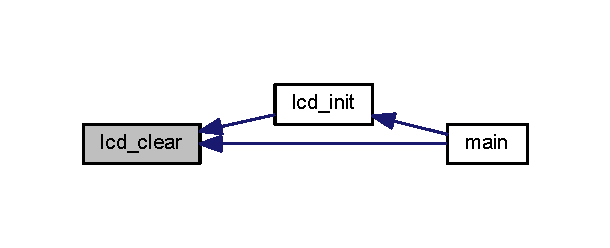
\includegraphics[width=350pt]{lcd__driver_8c_ad235a86241458b1e7b8771688bfdaf9a_icgraph}
\end{center}
\end{figure}
\mbox{\Hypertarget{lcd__driver_8c_a6842775ba83d166f02b8fef8bb63b1e6}\label{lcd__driver_8c_a6842775ba83d166f02b8fef8bb63b1e6}} 
\index{lcd\+\_\+driver.\+c@{lcd\+\_\+driver.\+c}!lcd\+\_\+init@{lcd\+\_\+init}}
\index{lcd\+\_\+init@{lcd\+\_\+init}!lcd\+\_\+driver.\+c@{lcd\+\_\+driver.\+c}}
\subsubsection{\texorpdfstring{lcd\+\_\+init()}{lcd\_init()}}
{\footnotesize\ttfamily void lcd\+\_\+init (\begin{DoxyParamCaption}\item[{void}]{ }\end{DoxyParamCaption})}



Definition at line 139 of file lcd\+\_\+driver.\+c.

Here is the call graph for this function\+:\nopagebreak
\begin{figure}[H]
\begin{center}
\leavevmode
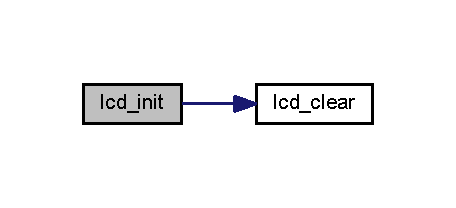
\includegraphics[width=219pt]{lcd__driver_8c_a6842775ba83d166f02b8fef8bb63b1e6_cgraph}
\end{center}
\end{figure}
Here is the caller graph for this function\+:\nopagebreak
\begin{figure}[H]
\begin{center}
\leavevmode
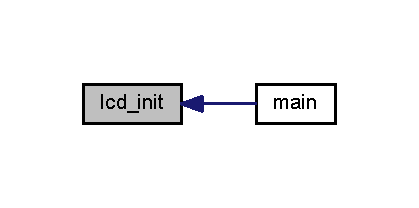
\includegraphics[width=285pt]{lcd__driver_8c_a6842775ba83d166f02b8fef8bb63b1e6_icgraph}
\end{center}
\end{figure}
\mbox{\Hypertarget{lcd__driver_8c_acc135402ee97c717da0e94d4f35ab220}\label{lcd__driver_8c_acc135402ee97c717da0e94d4f35ab220}} 
\index{lcd\+\_\+driver.\+c@{lcd\+\_\+driver.\+c}!lcd\+\_\+set\+Bar@{lcd\+\_\+set\+Bar}}
\index{lcd\+\_\+set\+Bar@{lcd\+\_\+set\+Bar}!lcd\+\_\+driver.\+c@{lcd\+\_\+driver.\+c}}
\subsubsection{\texorpdfstring{lcd\+\_\+set\+Bar()}{lcd\_setBar()}}
{\footnotesize\ttfamily void lcd\+\_\+set\+Bar (\begin{DoxyParamCaption}\item[{uint8\+\_\+t}]{x\+Position\+UL,  }\item[{uint8\+\_\+t}]{y\+Position\+UL,  }\item[{uint8\+\_\+t}]{x\+Position\+DR,  }\item[{uint8\+\_\+t}]{y\+Position\+DR }\end{DoxyParamCaption})}



Definition at line 266 of file lcd\+\_\+driver.\+c.

Here is the call graph for this function\+:\nopagebreak
\begin{figure}[H]
\begin{center}
\leavevmode
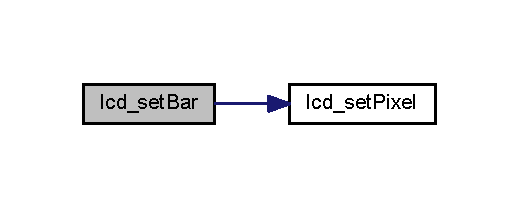
\includegraphics[width=249pt]{lcd__driver_8c_acc135402ee97c717da0e94d4f35ab220_cgraph}
\end{center}
\end{figure}
\mbox{\Hypertarget{lcd__driver_8c_a4f59541ea134603bee01a883f996e4ba}\label{lcd__driver_8c_a4f59541ea134603bee01a883f996e4ba}} 
\index{lcd\+\_\+driver.\+c@{lcd\+\_\+driver.\+c}!lcd\+\_\+set\+Char@{lcd\+\_\+set\+Char}}
\index{lcd\+\_\+set\+Char@{lcd\+\_\+set\+Char}!lcd\+\_\+driver.\+c@{lcd\+\_\+driver.\+c}}
\subsubsection{\texorpdfstring{lcd\+\_\+set\+Char()}{lcd\_setChar()}}
{\footnotesize\ttfamily void lcd\+\_\+set\+Char (\begin{DoxyParamCaption}\item[{uint8\+\_\+t}]{x\+Position,  }\item[{uint8\+\_\+t}]{y\+Position,  }\item[{unsigned char}]{char\+To\+Set,  }\item[{\mbox{\hyperlink{lcd__driver_8h_a438e9a5e935271711f6a0b377ba365fc}{lcd\+\_\+font\+Size}}}]{size,  }\item[{bool}]{contrast\+Is\+Inverted }\end{DoxyParamCaption})}



Definition at line 172 of file lcd\+\_\+driver.\+c.

Here is the caller graph for this function\+:\nopagebreak
\begin{figure}[H]
\begin{center}
\leavevmode
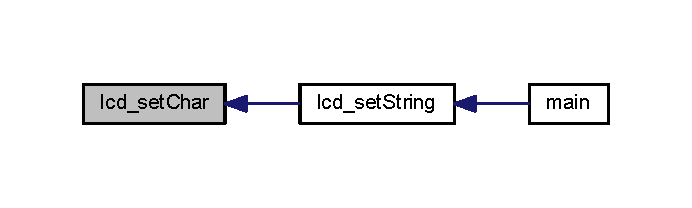
\includegraphics[width=263pt]{lcd__driver_8c_a4f59541ea134603bee01a883f996e4ba_icgraph}
\end{center}
\end{figure}
\mbox{\Hypertarget{lcd__driver_8c_a01af79135674b85725f569e8676b56ed}\label{lcd__driver_8c_a01af79135674b85725f569e8676b56ed}} 
\index{lcd\+\_\+driver.\+c@{lcd\+\_\+driver.\+c}!lcd\+\_\+set\+Contrast@{lcd\+\_\+set\+Contrast}}
\index{lcd\+\_\+set\+Contrast@{lcd\+\_\+set\+Contrast}!lcd\+\_\+driver.\+c@{lcd\+\_\+driver.\+c}}
\subsubsection{\texorpdfstring{lcd\+\_\+set\+Contrast()}{lcd\_setContrast()}}
{\footnotesize\ttfamily void lcd\+\_\+set\+Contrast (\begin{DoxyParamCaption}\item[{uint8\+\_\+t}]{electronic\+Volume }\end{DoxyParamCaption})}



Definition at line 128 of file lcd\+\_\+driver.\+c.

\mbox{\Hypertarget{lcd__driver_8c_a9bcf73809a621cc65f9ae004404ecf4e}\label{lcd__driver_8c_a9bcf73809a621cc65f9ae004404ecf4e}} 
\index{lcd\+\_\+driver.\+c@{lcd\+\_\+driver.\+c}!lcd\+\_\+set\+Frame@{lcd\+\_\+set\+Frame}}
\index{lcd\+\_\+set\+Frame@{lcd\+\_\+set\+Frame}!lcd\+\_\+driver.\+c@{lcd\+\_\+driver.\+c}}
\subsubsection{\texorpdfstring{lcd\+\_\+set\+Frame()}{lcd\_setFrame()}}
{\footnotesize\ttfamily void lcd\+\_\+set\+Frame (\begin{DoxyParamCaption}\item[{uint8\+\_\+t}]{x\+Position\+UL,  }\item[{uint8\+\_\+t}]{y\+Position\+UL,  }\item[{uint8\+\_\+t}]{x\+Position\+DR,  }\item[{uint8\+\_\+t}]{y\+Position\+DR }\end{DoxyParamCaption})}



Definition at line 253 of file lcd\+\_\+driver.\+c.

Here is the call graph for this function\+:\nopagebreak
\begin{figure}[H]
\begin{center}
\leavevmode
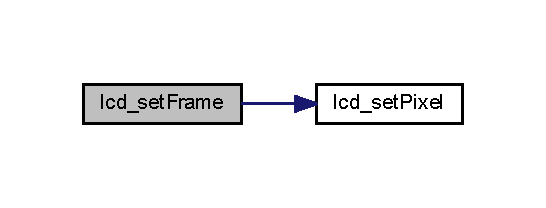
\includegraphics[width=262pt]{lcd__driver_8c_a9bcf73809a621cc65f9ae004404ecf4e_cgraph}
\end{center}
\end{figure}
\mbox{\Hypertarget{lcd__driver_8c_ae6ba6c6161cf3ec1ade0a72595cda0ce}\label{lcd__driver_8c_ae6ba6c6161cf3ec1ade0a72595cda0ce}} 
\index{lcd\+\_\+driver.\+c@{lcd\+\_\+driver.\+c}!lcd\+\_\+set\+Line@{lcd\+\_\+set\+Line}}
\index{lcd\+\_\+set\+Line@{lcd\+\_\+set\+Line}!lcd\+\_\+driver.\+c@{lcd\+\_\+driver.\+c}}
\subsubsection{\texorpdfstring{lcd\+\_\+set\+Line()}{lcd\_setLine()}}
{\footnotesize\ttfamily void lcd\+\_\+set\+Line (\begin{DoxyParamCaption}\item[{int16\+\_\+t}]{x1,  }\item[{int16\+\_\+t}]{y1,  }\item[{int16\+\_\+t}]{x2,  }\item[{int16\+\_\+t}]{y2,  }\item[{uint8\+\_\+t}]{state }\end{DoxyParamCaption})}



Definition at line 212 of file lcd\+\_\+driver.\+c.

Here is the call graph for this function\+:\nopagebreak
\begin{figure}[H]
\begin{center}
\leavevmode
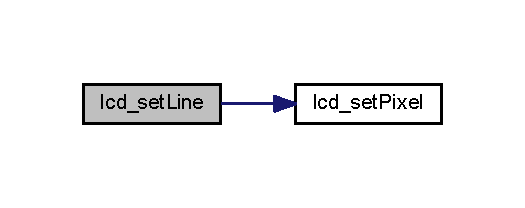
\includegraphics[width=252pt]{lcd__driver_8c_ae6ba6c6161cf3ec1ade0a72595cda0ce_cgraph}
\end{center}
\end{figure}
\mbox{\Hypertarget{lcd__driver_8c_aa76a5521efe086a9d26cbf44af732e8b}\label{lcd__driver_8c_aa76a5521efe086a9d26cbf44af732e8b}} 
\index{lcd\+\_\+driver.\+c@{lcd\+\_\+driver.\+c}!lcd\+\_\+set\+Pixel@{lcd\+\_\+set\+Pixel}}
\index{lcd\+\_\+set\+Pixel@{lcd\+\_\+set\+Pixel}!lcd\+\_\+driver.\+c@{lcd\+\_\+driver.\+c}}
\subsubsection{\texorpdfstring{lcd\+\_\+set\+Pixel()}{lcd\_setPixel()}}
{\footnotesize\ttfamily void lcd\+\_\+set\+Pixel (\begin{DoxyParamCaption}\item[{uint8\+\_\+t}]{x\+Position,  }\item[{uint8\+\_\+t}]{y\+Position,  }\item[{bool}]{pixel\+Is\+Set }\end{DoxyParamCaption})}



Definition at line 154 of file lcd\+\_\+driver.\+c.

Here is the caller graph for this function\+:\nopagebreak
\begin{figure}[H]
\begin{center}
\leavevmode
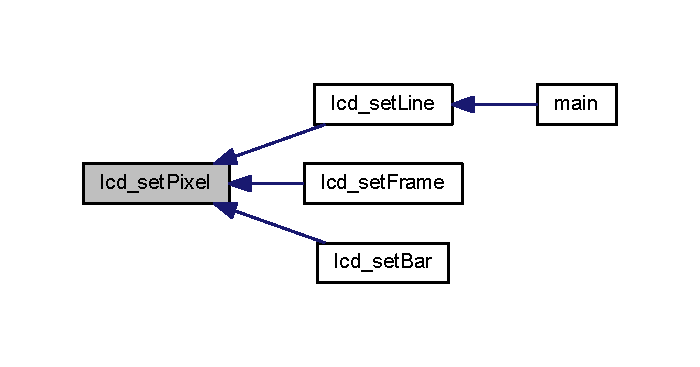
\includegraphics[width=350pt]{lcd__driver_8c_aa76a5521efe086a9d26cbf44af732e8b_icgraph}
\end{center}
\end{figure}
\mbox{\Hypertarget{lcd__driver_8c_aa6b1e5b4910ace65815c78a3da51f964}\label{lcd__driver_8c_aa6b1e5b4910ace65815c78a3da51f964}} 
\index{lcd\+\_\+driver.\+c@{lcd\+\_\+driver.\+c}!lcd\+\_\+set\+String@{lcd\+\_\+set\+String}}
\index{lcd\+\_\+set\+String@{lcd\+\_\+set\+String}!lcd\+\_\+driver.\+c@{lcd\+\_\+driver.\+c}}
\subsubsection{\texorpdfstring{lcd\+\_\+set\+String()}{lcd\_setString()}}
{\footnotesize\ttfamily void lcd\+\_\+set\+String (\begin{DoxyParamCaption}\item[{uint8\+\_\+t}]{x\+Position,  }\item[{uint8\+\_\+t}]{y\+Position,  }\item[{char const $\ast$}]{string,  }\item[{\mbox{\hyperlink{lcd__driver_8h_a438e9a5e935271711f6a0b377ba365fc}{lcd\+\_\+font\+Size}}}]{size,  }\item[{bool}]{contrast\+Is\+Inverted }\end{DoxyParamCaption})}



Definition at line 190 of file lcd\+\_\+driver.\+c.

Here is the call graph for this function\+:\nopagebreak
\begin{figure}[H]
\begin{center}
\leavevmode
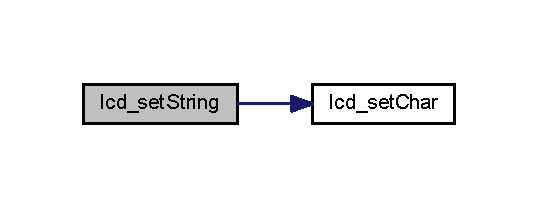
\includegraphics[width=258pt]{lcd__driver_8c_aa6b1e5b4910ace65815c78a3da51f964_cgraph}
\end{center}
\end{figure}
\mbox{\Hypertarget{lcd__driver_8c_aceada75059c9ce992fa7e7f38bea8fb3}\label{lcd__driver_8c_aceada75059c9ce992fa7e7f38bea8fb3}} 
\index{lcd\+\_\+driver.\+c@{lcd\+\_\+driver.\+c}!lcd\+\_\+set\+String2@{lcd\+\_\+set\+String2}}
\index{lcd\+\_\+set\+String2@{lcd\+\_\+set\+String2}!lcd\+\_\+driver.\+c@{lcd\+\_\+driver.\+c}}
\subsubsection{\texorpdfstring{lcd\+\_\+set\+String2()}{lcd\_setString2()}}
{\footnotesize\ttfamily void lcd\+\_\+set\+String2 (\begin{DoxyParamCaption}\item[{uint8\+\_\+t}]{x\+Position,  }\item[{uint8\+\_\+t}]{y\+Position,  }\item[{char const $\ast$}]{string,  }\item[{\mbox{\hyperlink{lcd__driver_8h_a438e9a5e935271711f6a0b377ba365fc}{lcd\+\_\+font\+Size}}}]{size,  }\item[{bool}]{contrast\+Is\+Inverted }\end{DoxyParamCaption})}



Definition at line 201 of file lcd\+\_\+driver.\+c.

Here is the call graph for this function\+:\nopagebreak
\begin{figure}[H]
\begin{center}
\leavevmode
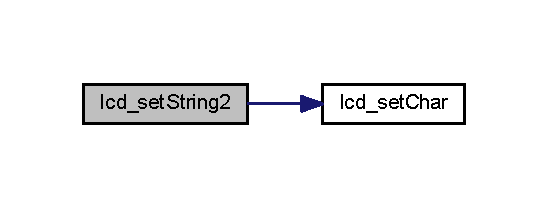
\includegraphics[width=263pt]{lcd__driver_8c_aceada75059c9ce992fa7e7f38bea8fb3_cgraph}
\end{center}
\end{figure}
\mbox{\Hypertarget{lcd__driver_8c_a1b56ac880918035df02119018094cfdb}\label{lcd__driver_8c_a1b56ac880918035df02119018094cfdb}} 
\index{lcd\+\_\+driver.\+c@{lcd\+\_\+driver.\+c}!lcd\+\_\+set\+Symbol8@{lcd\+\_\+set\+Symbol8}}
\index{lcd\+\_\+set\+Symbol8@{lcd\+\_\+set\+Symbol8}!lcd\+\_\+driver.\+c@{lcd\+\_\+driver.\+c}}
\subsubsection{\texorpdfstring{lcd\+\_\+set\+Symbol8()}{lcd\_setSymbol8()}}
{\footnotesize\ttfamily void lcd\+\_\+set\+Symbol8 (\begin{DoxyParamCaption}\item[{uint8\+\_\+t}]{x\+Position,  }\item[{uint8\+\_\+t}]{y\+Position,  }\item[{\mbox{\hyperlink{lcd__driver_8h_a85e540e9ffc9be3c6e946ccfc7dd2358}{lcd\+\_\+symbol}}}]{symbol,  }\item[{bool}]{contrast\+Is\+Inverted }\end{DoxyParamCaption})}



Definition at line 274 of file lcd\+\_\+driver.\+c.

\mbox{\Hypertarget{lcd__driver_8c_a3d045005d00fc4525d582d0f7559a313}\label{lcd__driver_8c_a3d045005d00fc4525d582d0f7559a313}} 
\index{lcd\+\_\+driver.\+c@{lcd\+\_\+driver.\+c}!lcd\+\_\+show@{lcd\+\_\+show}}
\index{lcd\+\_\+show@{lcd\+\_\+show}!lcd\+\_\+driver.\+c@{lcd\+\_\+driver.\+c}}
\subsubsection{\texorpdfstring{lcd\+\_\+show()}{lcd\_show()}}
{\footnotesize\ttfamily void lcd\+\_\+show (\begin{DoxyParamCaption}\item[{void}]{ }\end{DoxyParamCaption})}



Definition at line 242 of file lcd\+\_\+driver.\+c.

Here is the caller graph for this function\+:\nopagebreak
\begin{figure}[H]
\begin{center}
\leavevmode
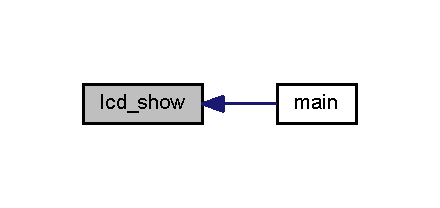
\includegraphics[width=280pt]{lcd__driver_8c_a3d045005d00fc4525d582d0f7559a313_icgraph}
\end{center}
\end{figure}
\mbox{\Hypertarget{lcd__driver_8c_a5a18286d5a8b9cb3a7149987b595fc03}\label{lcd__driver_8c_a5a18286d5a8b9cb3a7149987b595fc03}} 
\index{lcd\+\_\+driver.\+c@{lcd\+\_\+driver.\+c}!send\+Data@{send\+Data}}
\index{send\+Data@{send\+Data}!lcd\+\_\+driver.\+c@{lcd\+\_\+driver.\+c}}
\subsubsection{\texorpdfstring{send\+Data()}{sendData()}}
{\footnotesize\ttfamily void send\+Data (\begin{DoxyParamCaption}\item[{uint8\+\_\+t}]{data }\end{DoxyParamCaption})}



Definition at line 120 of file lcd\+\_\+driver.\+c.


\hypertarget{lcd__menu_8c}{}\section{Library/\+Library/src/lcd\+\_\+menu.c File Reference}
\label{lcd__menu_8c}\index{Library/\+Library/src/lcd\+\_\+menu.\+c@{Library/\+Library/src/lcd\+\_\+menu.\+c}}
{\ttfamily \#include \char`\"{}lcd\+\_\+menu.\+h\char`\"{}}\newline
{\ttfamily \#include $<$stdbool.\+h$>$}\newline
Include dependency graph for lcd\+\_\+menu.\+c\+:\nopagebreak
\begin{figure}[H]
\begin{center}
\leavevmode
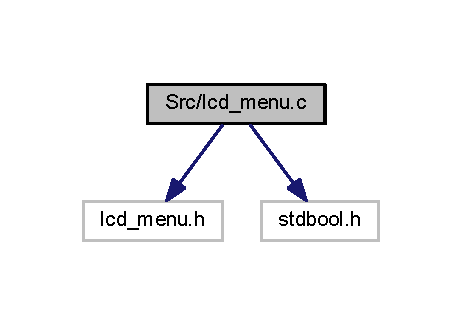
\includegraphics[width=347pt]{lcd__menu_8c__incl}
\end{center}
\end{figure}
\subsection*{Macros}
\begin{DoxyCompactItemize}
\item 
\#define \mbox{\hyperlink{lcd__menu_8c_a5ec6c1d7718fbdddb575f6ba208b663b}{E\+N\+T\+R\+I\+E\+S\+\_\+\+P\+E\+R\+\_\+\+P\+A\+GE}}~((uint8\+\_\+t) 3)
\item 
\#define \mbox{\hyperlink{lcd__menu_8c_a4d07ded3da9fcfd610698b7988a36716}{S\+C\+R\+O\+L\+L\+B\+A\+R\+\_\+\+M\+A\+X\+\_\+\+H\+A\+N\+D\+L\+E\+\_\+\+H\+E\+I\+G\+HT}}~((uint8\+\_\+t) 27)
\item 
\#define \mbox{\hyperlink{lcd__menu_8c_a5b435ea89853f94197c9b84e1307a145}{S\+C\+R\+O\+L\+L\+B\+A\+R\+\_\+\+H\+A\+N\+D\+L\+E\+\_\+\+W\+I\+D\+TH}}~((uint8\+\_\+t) 2)
\item 
\#define \mbox{\hyperlink{lcd__menu_8c_a7ae0d8a7b30bb419e5b48035e9c9318b}{S\+C\+R\+O\+L\+L\+B\+A\+R\+\_\+\+H\+A\+N\+D\+L\+E\+\_\+\+A\+N\+C\+H\+O\+R\+\_\+X}}~((uint8\+\_\+t) 123)
\item 
\#define \mbox{\hyperlink{lcd__menu_8c_a7cf6b09609b0305ab16e50614b668c87}{S\+C\+R\+O\+L\+L\+B\+A\+R\+\_\+\+H\+A\+N\+D\+L\+E\+\_\+\+A\+N\+C\+H\+O\+R\+\_\+Y}}~((uint8\+\_\+t) 2)
\item 
\#define \mbox{\hyperlink{lcd__menu_8c_a16777040de931fea6aa6688ae9db7ad3}{S\+C\+R\+O\+L\+L\+B\+A\+R\+\_\+\+F\+R\+A\+M\+E\+\_\+\+T\+O\+P\+\_\+\+L\+E\+F\+T\+\_\+X}}~((uint8\+\_\+t) 121)
\item 
\#define \mbox{\hyperlink{lcd__menu_8c_ae004905def783b08724e4e0cd620867e}{S\+C\+R\+O\+L\+L\+B\+A\+R\+\_\+\+F\+R\+A\+M\+E\+\_\+\+T\+O\+P\+\_\+\+L\+E\+F\+T\+\_\+Y}}~((uint8\+\_\+t) 0)
\item 
\#define \mbox{\hyperlink{lcd__menu_8c_ae7214440d0ef700f3325b245f4cd919b}{S\+C\+R\+O\+L\+L\+B\+A\+R\+\_\+\+F\+R\+A\+M\+E\+\_\+\+B\+O\+T\+T\+O\+M\+\_\+\+R\+I\+G\+H\+T\+\_\+X}}~((uint8\+\_\+t) 127)
\item 
\#define \mbox{\hyperlink{lcd__menu_8c_a61b3e5005118f6d618c4423f2e072ea7}{S\+C\+R\+O\+L\+L\+B\+A\+R\+\_\+\+F\+R\+A\+M\+E\+\_\+\+B\+O\+T\+T\+O\+M\+\_\+\+R\+I\+G\+H\+T\+\_\+Y}}~((uint8\+\_\+t) 31)
\end{DoxyCompactItemize}
\subsection*{Functions}
\begin{DoxyCompactItemize}
\item 
void \mbox{\hyperlink{lcd__menu_8c_a241201125b49b0478d339a7c3a9f8f5a}{menu\+\_\+set\+Main\+Menu}} (\mbox{\hyperlink{lcd__menu_8h_afe0ab1c0311f677767b1588296b0f563}{Menu}} $\ast$const menu)
\item 
void \mbox{\hyperlink{lcd__menu_8c_a375ecfefafd703a57877c819e5c0c698}{menu\+\_\+register\+Draw\+Menu\+Item2}} (\mbox{\hyperlink{lcd__menu_8h_af336c49ff8310ef7d0eef6c8148e2317}{menu\+User\+Draw\+Item2}} func, void $\ast$data)
\item 
void \mbox{\hyperlink{lcd__menu_8c_aacbd3ab5885aa663bfae18f8ba403d14}{menu\+\_\+show}} ()
\item 
\mbox{\hyperlink{lcd__menu_8h_af281888756940391027a7bdddf347718}{menu\+\_\+event}} \mbox{\hyperlink{lcd__menu_8c_a90ddf7b832aa21b33f2b27e7787e6329}{menu\+\_\+update}} (\mbox{\hyperlink{lcd__menu_8h_acc7822c56ab54b113c6a9ee3d7fea165}{menu\+\_\+navigation}} navigation)
\end{DoxyCompactItemize}


\subsection{Macro Definition Documentation}
\mbox{\Hypertarget{lcd__menu_8c_a5ec6c1d7718fbdddb575f6ba208b663b}\label{lcd__menu_8c_a5ec6c1d7718fbdddb575f6ba208b663b}} 
\index{lcd\+\_\+menu.\+c@{lcd\+\_\+menu.\+c}!E\+N\+T\+R\+I\+E\+S\+\_\+\+P\+E\+R\+\_\+\+P\+A\+GE@{E\+N\+T\+R\+I\+E\+S\+\_\+\+P\+E\+R\+\_\+\+P\+A\+GE}}
\index{E\+N\+T\+R\+I\+E\+S\+\_\+\+P\+E\+R\+\_\+\+P\+A\+GE@{E\+N\+T\+R\+I\+E\+S\+\_\+\+P\+E\+R\+\_\+\+P\+A\+GE}!lcd\+\_\+menu.\+c@{lcd\+\_\+menu.\+c}}
\subsubsection{\texorpdfstring{E\+N\+T\+R\+I\+E\+S\+\_\+\+P\+E\+R\+\_\+\+P\+A\+GE}{ENTRIES\_PER\_PAGE}}
{\footnotesize\ttfamily \#define E\+N\+T\+R\+I\+E\+S\+\_\+\+P\+E\+R\+\_\+\+P\+A\+GE~((uint8\+\_\+t) 3)}



Definition at line 4 of file lcd\+\_\+menu.\+c.

\mbox{\Hypertarget{lcd__menu_8c_ae7214440d0ef700f3325b245f4cd919b}\label{lcd__menu_8c_ae7214440d0ef700f3325b245f4cd919b}} 
\index{lcd\+\_\+menu.\+c@{lcd\+\_\+menu.\+c}!S\+C\+R\+O\+L\+L\+B\+A\+R\+\_\+\+F\+R\+A\+M\+E\+\_\+\+B\+O\+T\+T\+O\+M\+\_\+\+R\+I\+G\+H\+T\+\_\+X@{S\+C\+R\+O\+L\+L\+B\+A\+R\+\_\+\+F\+R\+A\+M\+E\+\_\+\+B\+O\+T\+T\+O\+M\+\_\+\+R\+I\+G\+H\+T\+\_\+X}}
\index{S\+C\+R\+O\+L\+L\+B\+A\+R\+\_\+\+F\+R\+A\+M\+E\+\_\+\+B\+O\+T\+T\+O\+M\+\_\+\+R\+I\+G\+H\+T\+\_\+X@{S\+C\+R\+O\+L\+L\+B\+A\+R\+\_\+\+F\+R\+A\+M\+E\+\_\+\+B\+O\+T\+T\+O\+M\+\_\+\+R\+I\+G\+H\+T\+\_\+X}!lcd\+\_\+menu.\+c@{lcd\+\_\+menu.\+c}}
\subsubsection{\texorpdfstring{S\+C\+R\+O\+L\+L\+B\+A\+R\+\_\+\+F\+R\+A\+M\+E\+\_\+\+B\+O\+T\+T\+O\+M\+\_\+\+R\+I\+G\+H\+T\+\_\+X}{SCROLLBAR\_FRAME\_BOTTOM\_RIGHT\_X}}
{\footnotesize\ttfamily \#define S\+C\+R\+O\+L\+L\+B\+A\+R\+\_\+\+F\+R\+A\+M\+E\+\_\+\+B\+O\+T\+T\+O\+M\+\_\+\+R\+I\+G\+H\+T\+\_\+X~((uint8\+\_\+t) 127)}

\mbox{\Hypertarget{lcd__menu_8c_a61b3e5005118f6d618c4423f2e072ea7}\label{lcd__menu_8c_a61b3e5005118f6d618c4423f2e072ea7}} 
\index{lcd\+\_\+menu.\+c@{lcd\+\_\+menu.\+c}!S\+C\+R\+O\+L\+L\+B\+A\+R\+\_\+\+F\+R\+A\+M\+E\+\_\+\+B\+O\+T\+T\+O\+M\+\_\+\+R\+I\+G\+H\+T\+\_\+Y@{S\+C\+R\+O\+L\+L\+B\+A\+R\+\_\+\+F\+R\+A\+M\+E\+\_\+\+B\+O\+T\+T\+O\+M\+\_\+\+R\+I\+G\+H\+T\+\_\+Y}}
\index{S\+C\+R\+O\+L\+L\+B\+A\+R\+\_\+\+F\+R\+A\+M\+E\+\_\+\+B\+O\+T\+T\+O\+M\+\_\+\+R\+I\+G\+H\+T\+\_\+Y@{S\+C\+R\+O\+L\+L\+B\+A\+R\+\_\+\+F\+R\+A\+M\+E\+\_\+\+B\+O\+T\+T\+O\+M\+\_\+\+R\+I\+G\+H\+T\+\_\+Y}!lcd\+\_\+menu.\+c@{lcd\+\_\+menu.\+c}}
\subsubsection{\texorpdfstring{S\+C\+R\+O\+L\+L\+B\+A\+R\+\_\+\+F\+R\+A\+M\+E\+\_\+\+B\+O\+T\+T\+O\+M\+\_\+\+R\+I\+G\+H\+T\+\_\+Y}{SCROLLBAR\_FRAME\_BOTTOM\_RIGHT\_Y}}
{\footnotesize\ttfamily \#define S\+C\+R\+O\+L\+L\+B\+A\+R\+\_\+\+F\+R\+A\+M\+E\+\_\+\+B\+O\+T\+T\+O\+M\+\_\+\+R\+I\+G\+H\+T\+\_\+Y~((uint8\+\_\+t) 31)}

\mbox{\Hypertarget{lcd__menu_8c_a16777040de931fea6aa6688ae9db7ad3}\label{lcd__menu_8c_a16777040de931fea6aa6688ae9db7ad3}} 
\index{lcd\+\_\+menu.\+c@{lcd\+\_\+menu.\+c}!S\+C\+R\+O\+L\+L\+B\+A\+R\+\_\+\+F\+R\+A\+M\+E\+\_\+\+T\+O\+P\+\_\+\+L\+E\+F\+T\+\_\+X@{S\+C\+R\+O\+L\+L\+B\+A\+R\+\_\+\+F\+R\+A\+M\+E\+\_\+\+T\+O\+P\+\_\+\+L\+E\+F\+T\+\_\+X}}
\index{S\+C\+R\+O\+L\+L\+B\+A\+R\+\_\+\+F\+R\+A\+M\+E\+\_\+\+T\+O\+P\+\_\+\+L\+E\+F\+T\+\_\+X@{S\+C\+R\+O\+L\+L\+B\+A\+R\+\_\+\+F\+R\+A\+M\+E\+\_\+\+T\+O\+P\+\_\+\+L\+E\+F\+T\+\_\+X}!lcd\+\_\+menu.\+c@{lcd\+\_\+menu.\+c}}
\subsubsection{\texorpdfstring{S\+C\+R\+O\+L\+L\+B\+A\+R\+\_\+\+F\+R\+A\+M\+E\+\_\+\+T\+O\+P\+\_\+\+L\+E\+F\+T\+\_\+X}{SCROLLBAR\_FRAME\_TOP\_LEFT\_X}}
{\footnotesize\ttfamily \#define S\+C\+R\+O\+L\+L\+B\+A\+R\+\_\+\+F\+R\+A\+M\+E\+\_\+\+T\+O\+P\+\_\+\+L\+E\+F\+T\+\_\+X~((uint8\+\_\+t) 121)}

\mbox{\Hypertarget{lcd__menu_8c_ae004905def783b08724e4e0cd620867e}\label{lcd__menu_8c_ae004905def783b08724e4e0cd620867e}} 
\index{lcd\+\_\+menu.\+c@{lcd\+\_\+menu.\+c}!S\+C\+R\+O\+L\+L\+B\+A\+R\+\_\+\+F\+R\+A\+M\+E\+\_\+\+T\+O\+P\+\_\+\+L\+E\+F\+T\+\_\+Y@{S\+C\+R\+O\+L\+L\+B\+A\+R\+\_\+\+F\+R\+A\+M\+E\+\_\+\+T\+O\+P\+\_\+\+L\+E\+F\+T\+\_\+Y}}
\index{S\+C\+R\+O\+L\+L\+B\+A\+R\+\_\+\+F\+R\+A\+M\+E\+\_\+\+T\+O\+P\+\_\+\+L\+E\+F\+T\+\_\+Y@{S\+C\+R\+O\+L\+L\+B\+A\+R\+\_\+\+F\+R\+A\+M\+E\+\_\+\+T\+O\+P\+\_\+\+L\+E\+F\+T\+\_\+Y}!lcd\+\_\+menu.\+c@{lcd\+\_\+menu.\+c}}
\subsubsection{\texorpdfstring{S\+C\+R\+O\+L\+L\+B\+A\+R\+\_\+\+F\+R\+A\+M\+E\+\_\+\+T\+O\+P\+\_\+\+L\+E\+F\+T\+\_\+Y}{SCROLLBAR\_FRAME\_TOP\_LEFT\_Y}}
{\footnotesize\ttfamily \#define S\+C\+R\+O\+L\+L\+B\+A\+R\+\_\+\+F\+R\+A\+M\+E\+\_\+\+T\+O\+P\+\_\+\+L\+E\+F\+T\+\_\+Y~((uint8\+\_\+t) 0)}

\mbox{\Hypertarget{lcd__menu_8c_a7ae0d8a7b30bb419e5b48035e9c9318b}\label{lcd__menu_8c_a7ae0d8a7b30bb419e5b48035e9c9318b}} 
\index{lcd\+\_\+menu.\+c@{lcd\+\_\+menu.\+c}!S\+C\+R\+O\+L\+L\+B\+A\+R\+\_\+\+H\+A\+N\+D\+L\+E\+\_\+\+A\+N\+C\+H\+O\+R\+\_\+X@{S\+C\+R\+O\+L\+L\+B\+A\+R\+\_\+\+H\+A\+N\+D\+L\+E\+\_\+\+A\+N\+C\+H\+O\+R\+\_\+X}}
\index{S\+C\+R\+O\+L\+L\+B\+A\+R\+\_\+\+H\+A\+N\+D\+L\+E\+\_\+\+A\+N\+C\+H\+O\+R\+\_\+X@{S\+C\+R\+O\+L\+L\+B\+A\+R\+\_\+\+H\+A\+N\+D\+L\+E\+\_\+\+A\+N\+C\+H\+O\+R\+\_\+X}!lcd\+\_\+menu.\+c@{lcd\+\_\+menu.\+c}}
\subsubsection{\texorpdfstring{S\+C\+R\+O\+L\+L\+B\+A\+R\+\_\+\+H\+A\+N\+D\+L\+E\+\_\+\+A\+N\+C\+H\+O\+R\+\_\+X}{SCROLLBAR\_HANDLE\_ANCHOR\_X}}
{\footnotesize\ttfamily \#define S\+C\+R\+O\+L\+L\+B\+A\+R\+\_\+\+H\+A\+N\+D\+L\+E\+\_\+\+A\+N\+C\+H\+O\+R\+\_\+X~((uint8\+\_\+t) 123)}

\mbox{\Hypertarget{lcd__menu_8c_a7cf6b09609b0305ab16e50614b668c87}\label{lcd__menu_8c_a7cf6b09609b0305ab16e50614b668c87}} 
\index{lcd\+\_\+menu.\+c@{lcd\+\_\+menu.\+c}!S\+C\+R\+O\+L\+L\+B\+A\+R\+\_\+\+H\+A\+N\+D\+L\+E\+\_\+\+A\+N\+C\+H\+O\+R\+\_\+Y@{S\+C\+R\+O\+L\+L\+B\+A\+R\+\_\+\+H\+A\+N\+D\+L\+E\+\_\+\+A\+N\+C\+H\+O\+R\+\_\+Y}}
\index{S\+C\+R\+O\+L\+L\+B\+A\+R\+\_\+\+H\+A\+N\+D\+L\+E\+\_\+\+A\+N\+C\+H\+O\+R\+\_\+Y@{S\+C\+R\+O\+L\+L\+B\+A\+R\+\_\+\+H\+A\+N\+D\+L\+E\+\_\+\+A\+N\+C\+H\+O\+R\+\_\+Y}!lcd\+\_\+menu.\+c@{lcd\+\_\+menu.\+c}}
\subsubsection{\texorpdfstring{S\+C\+R\+O\+L\+L\+B\+A\+R\+\_\+\+H\+A\+N\+D\+L\+E\+\_\+\+A\+N\+C\+H\+O\+R\+\_\+Y}{SCROLLBAR\_HANDLE\_ANCHOR\_Y}}
{\footnotesize\ttfamily \#define S\+C\+R\+O\+L\+L\+B\+A\+R\+\_\+\+H\+A\+N\+D\+L\+E\+\_\+\+A\+N\+C\+H\+O\+R\+\_\+Y~((uint8\+\_\+t) 2)}

\mbox{\Hypertarget{lcd__menu_8c_a5b435ea89853f94197c9b84e1307a145}\label{lcd__menu_8c_a5b435ea89853f94197c9b84e1307a145}} 
\index{lcd\+\_\+menu.\+c@{lcd\+\_\+menu.\+c}!S\+C\+R\+O\+L\+L\+B\+A\+R\+\_\+\+H\+A\+N\+D\+L\+E\+\_\+\+W\+I\+D\+TH@{S\+C\+R\+O\+L\+L\+B\+A\+R\+\_\+\+H\+A\+N\+D\+L\+E\+\_\+\+W\+I\+D\+TH}}
\index{S\+C\+R\+O\+L\+L\+B\+A\+R\+\_\+\+H\+A\+N\+D\+L\+E\+\_\+\+W\+I\+D\+TH@{S\+C\+R\+O\+L\+L\+B\+A\+R\+\_\+\+H\+A\+N\+D\+L\+E\+\_\+\+W\+I\+D\+TH}!lcd\+\_\+menu.\+c@{lcd\+\_\+menu.\+c}}
\subsubsection{\texorpdfstring{S\+C\+R\+O\+L\+L\+B\+A\+R\+\_\+\+H\+A\+N\+D\+L\+E\+\_\+\+W\+I\+D\+TH}{SCROLLBAR\_HANDLE\_WIDTH}}
{\footnotesize\ttfamily \#define S\+C\+R\+O\+L\+L\+B\+A\+R\+\_\+\+H\+A\+N\+D\+L\+E\+\_\+\+W\+I\+D\+TH~((uint8\+\_\+t) 2)}

\mbox{\Hypertarget{lcd__menu_8c_a4d07ded3da9fcfd610698b7988a36716}\label{lcd__menu_8c_a4d07ded3da9fcfd610698b7988a36716}} 
\index{lcd\+\_\+menu.\+c@{lcd\+\_\+menu.\+c}!S\+C\+R\+O\+L\+L\+B\+A\+R\+\_\+\+M\+A\+X\+\_\+\+H\+A\+N\+D\+L\+E\+\_\+\+H\+E\+I\+G\+HT@{S\+C\+R\+O\+L\+L\+B\+A\+R\+\_\+\+M\+A\+X\+\_\+\+H\+A\+N\+D\+L\+E\+\_\+\+H\+E\+I\+G\+HT}}
\index{S\+C\+R\+O\+L\+L\+B\+A\+R\+\_\+\+M\+A\+X\+\_\+\+H\+A\+N\+D\+L\+E\+\_\+\+H\+E\+I\+G\+HT@{S\+C\+R\+O\+L\+L\+B\+A\+R\+\_\+\+M\+A\+X\+\_\+\+H\+A\+N\+D\+L\+E\+\_\+\+H\+E\+I\+G\+HT}!lcd\+\_\+menu.\+c@{lcd\+\_\+menu.\+c}}
\subsubsection{\texorpdfstring{S\+C\+R\+O\+L\+L\+B\+A\+R\+\_\+\+M\+A\+X\+\_\+\+H\+A\+N\+D\+L\+E\+\_\+\+H\+E\+I\+G\+HT}{SCROLLBAR\_MAX\_HANDLE\_HEIGHT}}
{\footnotesize\ttfamily \#define S\+C\+R\+O\+L\+L\+B\+A\+R\+\_\+\+M\+A\+X\+\_\+\+H\+A\+N\+D\+L\+E\+\_\+\+H\+E\+I\+G\+HT~((uint8\+\_\+t) 27)}



\subsection{Function Documentation}
\mbox{\Hypertarget{lcd__menu_8c_a375ecfefafd703a57877c819e5c0c698}\label{lcd__menu_8c_a375ecfefafd703a57877c819e5c0c698}} 
\index{lcd\+\_\+menu.\+c@{lcd\+\_\+menu.\+c}!menu\+\_\+register\+Draw\+Menu\+Item2@{menu\+\_\+register\+Draw\+Menu\+Item2}}
\index{menu\+\_\+register\+Draw\+Menu\+Item2@{menu\+\_\+register\+Draw\+Menu\+Item2}!lcd\+\_\+menu.\+c@{lcd\+\_\+menu.\+c}}
\subsubsection{\texorpdfstring{menu\+\_\+register\+Draw\+Menu\+Item2()}{menu\_registerDrawMenuItem2()}}
{\footnotesize\ttfamily void menu\+\_\+register\+Draw\+Menu\+Item2 (\begin{DoxyParamCaption}\item[{\mbox{\hyperlink{lcd__menu_8h_af336c49ff8310ef7d0eef6c8148e2317}{menu\+User\+Draw\+Item2}}}]{func,  }\item[{void $\ast$}]{data }\end{DoxyParamCaption})}



Definition at line 83 of file lcd\+\_\+menu.\+c.

Here is the caller graph for this function\+:\nopagebreak
\begin{figure}[H]
\begin{center}
\leavevmode
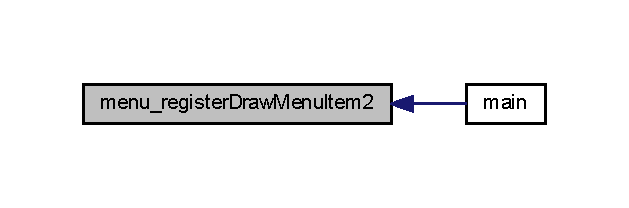
\includegraphics[width=302pt]{lcd__menu_8c_a375ecfefafd703a57877c819e5c0c698_icgraph}
\end{center}
\end{figure}
\mbox{\Hypertarget{lcd__menu_8c_a241201125b49b0478d339a7c3a9f8f5a}\label{lcd__menu_8c_a241201125b49b0478d339a7c3a9f8f5a}} 
\index{lcd\+\_\+menu.\+c@{lcd\+\_\+menu.\+c}!menu\+\_\+set\+Main\+Menu@{menu\+\_\+set\+Main\+Menu}}
\index{menu\+\_\+set\+Main\+Menu@{menu\+\_\+set\+Main\+Menu}!lcd\+\_\+menu.\+c@{lcd\+\_\+menu.\+c}}
\subsubsection{\texorpdfstring{menu\+\_\+set\+Main\+Menu()}{menu\_setMainMenu()}}
{\footnotesize\ttfamily void menu\+\_\+set\+Main\+Menu (\begin{DoxyParamCaption}\item[{\mbox{\hyperlink{lcd__menu_8h_afe0ab1c0311f677767b1588296b0f563}{Menu}} $\ast$const}]{menu }\end{DoxyParamCaption})}



Definition at line 10 of file lcd\+\_\+menu.\+c.

Here is the caller graph for this function\+:\nopagebreak
\begin{figure}[H]
\begin{center}
\leavevmode
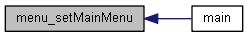
\includegraphics[width=258pt]{lcd__menu_8c_a241201125b49b0478d339a7c3a9f8f5a_icgraph}
\end{center}
\end{figure}
\mbox{\Hypertarget{lcd__menu_8c_aacbd3ab5885aa663bfae18f8ba403d14}\label{lcd__menu_8c_aacbd3ab5885aa663bfae18f8ba403d14}} 
\index{lcd\+\_\+menu.\+c@{lcd\+\_\+menu.\+c}!menu\+\_\+show@{menu\+\_\+show}}
\index{menu\+\_\+show@{menu\+\_\+show}!lcd\+\_\+menu.\+c@{lcd\+\_\+menu.\+c}}
\subsubsection{\texorpdfstring{menu\+\_\+show()}{menu\_show()}}
{\footnotesize\ttfamily void menu\+\_\+show (\begin{DoxyParamCaption}\item[{void}]{ }\end{DoxyParamCaption})}



Definition at line 106 of file lcd\+\_\+menu.\+c.

\mbox{\Hypertarget{lcd__menu_8c_a90ddf7b832aa21b33f2b27e7787e6329}\label{lcd__menu_8c_a90ddf7b832aa21b33f2b27e7787e6329}} 
\index{lcd\+\_\+menu.\+c@{lcd\+\_\+menu.\+c}!menu\+\_\+update@{menu\+\_\+update}}
\index{menu\+\_\+update@{menu\+\_\+update}!lcd\+\_\+menu.\+c@{lcd\+\_\+menu.\+c}}
\subsubsection{\texorpdfstring{menu\+\_\+update()}{menu\_update()}}
{\footnotesize\ttfamily \mbox{\hyperlink{lcd__menu_8h_af281888756940391027a7bdddf347718}{menu\+\_\+event}} menu\+\_\+update (\begin{DoxyParamCaption}\item[{\mbox{\hyperlink{lcd__menu_8h_acc7822c56ab54b113c6a9ee3d7fea165}{menu\+\_\+navigation}}}]{navigation }\end{DoxyParamCaption})}



Definition at line 117 of file lcd\+\_\+menu.\+c.


\hypertarget{main_8c}{}\section{Src/main.c File Reference}
\label{main_8c}\index{Src/main.\+c@{Src/main.\+c}}


\+: Main program body  


{\ttfamily \#include \char`\"{}main.\+h\char`\"{}}\newline
{\ttfamily \#include \char`\"{}stm32f4xx\+\_\+hal.\+h\char`\"{}}\newline
{\ttfamily \#include \char`\"{}spi.\+h\char`\"{}}\newline
{\ttfamily \#include \char`\"{}gpio.\+h\char`\"{}}\newline
{\ttfamily \#include \char`\"{}lcd\+\_\+driver.\+h\char`\"{}}\newline
{\ttfamily \#include $<$stdbool.\+h$>$}\newline
{\ttfamily \#include $<$stdio.\+h$>$}\newline
Include dependency graph for main.\+c\+:\nopagebreak
\begin{figure}[H]
\begin{center}
\leavevmode
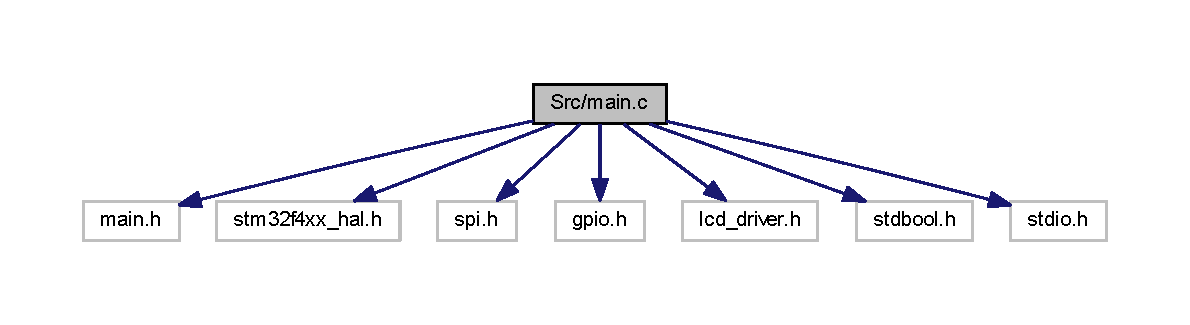
\includegraphics[width=350pt]{main_8c__incl}
\end{center}
\end{figure}
\subsection*{Functions}
\begin{DoxyCompactItemize}
\item 
void \mbox{\hyperlink{main_8c_a70af21c671abfcc773614a9a4f63d920}{System\+Clock\+\_\+\+Config}} (void)
\begin{DoxyCompactList}\small\item\em System Clock Configuration. \end{DoxyCompactList}\item 
int \mbox{\hyperlink{main_8c_a840291bc02cba5474a4cb46a9b9566fe}{main}} (void)
\begin{DoxyCompactList}\small\item\em That is Justing more un test about Doc application entry point. \end{DoxyCompactList}\item 
void \mbox{\hyperlink{main_8c_a829116a51f1db1a72ebd1120f60719d5}{\+\_\+\+Error\+\_\+\+Handler}} (char $\ast$file, int line)
\begin{DoxyCompactList}\small\item\em This function is executed in case of error occurrence. \end{DoxyCompactList}\end{DoxyCompactItemize}


\subsection{Detailed Description}
\+: Main program body 

This notice applies to any and all portions of this file that are not between comment pairs U\+S\+ER C\+O\+DE B\+E\+G\+IN and U\+S\+ER C\+O\+DE E\+ND. Other portions of this file, whether inserted by the user or by software development tools are owned by their respective copyright owners.

C\+O\+P\+Y\+R\+I\+G\+H\+T(c) 2018 S\+T\+Microelectronics

Redistribution and use in source and binary forms, with or without modification, are permitted provided that the following conditions are met\+:
\begin{DoxyEnumerate}
\item Redistributions of source code must retain the above copyright notice, this list of conditions and the following disclaimer.
\item Redistributions in binary form must reproduce the above copyright notice, this list of conditions and the following disclaimer in the documentation and/or other materials provided with the distribution.
\item Neither the name of S\+T\+Microelectronics nor the names of its contributors may be used to endorse or promote products derived from this software without specific prior written permission.
\end{DoxyEnumerate}

T\+H\+IS S\+O\+F\+T\+W\+A\+RE IS P\+R\+O\+V\+I\+D\+ED BY T\+HE C\+O\+P\+Y\+R\+I\+G\+HT H\+O\+L\+D\+E\+RS A\+ND C\+O\+N\+T\+R\+I\+B\+U\+T\+O\+RS \char`\"{}\+A\+S I\+S\char`\"{} A\+ND A\+NY E\+X\+P\+R\+E\+SS OR I\+M\+P\+L\+I\+ED W\+A\+R\+R\+A\+N\+T\+I\+ES, I\+N\+C\+L\+U\+D\+I\+NG, B\+UT N\+OT L\+I\+M\+I\+T\+ED TO, T\+HE I\+M\+P\+L\+I\+ED W\+A\+R\+R\+A\+N\+T\+I\+ES OF M\+E\+R\+C\+H\+A\+N\+T\+A\+B\+I\+L\+I\+TY A\+ND F\+I\+T\+N\+E\+SS F\+OR A P\+A\+R\+T\+I\+C\+U\+L\+AR P\+U\+R\+P\+O\+SE A\+RE D\+I\+S\+C\+L\+A\+I\+M\+ED. IN NO E\+V\+E\+NT S\+H\+A\+LL T\+HE C\+O\+P\+Y\+R\+I\+G\+HT H\+O\+L\+D\+ER OR C\+O\+N\+T\+R\+I\+B\+U\+T\+O\+RS BE L\+I\+A\+B\+LE F\+OR A\+NY D\+I\+R\+E\+CT, I\+N\+D\+I\+R\+E\+CT, I\+N\+C\+I\+D\+E\+N\+T\+AL, S\+P\+E\+C\+I\+AL, E\+X\+E\+M\+P\+L\+A\+RY, OR C\+O\+N\+S\+E\+Q\+U\+E\+N\+T\+I\+AL D\+A\+M\+A\+G\+ES (I\+N\+C\+L\+U\+D\+I\+NG, B\+UT N\+OT L\+I\+M\+I\+T\+ED TO, P\+R\+O\+C\+U\+R\+E\+M\+E\+NT OF S\+U\+B\+S\+T\+I\+T\+U\+TE G\+O\+O\+DS OR S\+E\+R\+V\+I\+C\+ES; L\+O\+SS OF U\+SE, D\+A\+TA, OR P\+R\+O\+F\+I\+TS; OR B\+U\+S\+I\+N\+E\+SS I\+N\+T\+E\+R\+R\+U\+P\+T\+I\+ON) H\+O\+W\+E\+V\+ER C\+A\+U\+S\+ED A\+ND ON A\+NY T\+H\+E\+O\+RY OF L\+I\+A\+B\+I\+L\+I\+TY, W\+H\+E\+T\+H\+ER IN C\+O\+N\+T\+R\+A\+CT, S\+T\+R\+I\+CT L\+I\+A\+B\+I\+L\+I\+TY, OR T\+O\+RT (I\+N\+C\+L\+U\+D\+I\+NG N\+E\+G\+L\+I\+G\+E\+N\+CE OR O\+T\+H\+E\+R\+W\+I\+SE) A\+R\+I\+S\+I\+NG IN A\+NY W\+AY O\+UT OF T\+HE U\+SE OF T\+H\+IS S\+O\+F\+T\+W\+A\+RE, E\+V\+EN IF A\+D\+V\+I\+S\+ED OF T\+HE P\+O\+S\+S\+I\+B\+I\+L\+I\+TY OF S\+U\+CH D\+A\+M\+A\+GE. 

\subsection{Function Documentation}
\mbox{\Hypertarget{main_8c_a829116a51f1db1a72ebd1120f60719d5}\label{main_8c_a829116a51f1db1a72ebd1120f60719d5}} 
\index{main.\+c@{main.\+c}!\+\_\+\+Error\+\_\+\+Handler@{\+\_\+\+Error\+\_\+\+Handler}}
\index{\+\_\+\+Error\+\_\+\+Handler@{\+\_\+\+Error\+\_\+\+Handler}!main.\+c@{main.\+c}}
\subsubsection{\texorpdfstring{\+\_\+\+Error\+\_\+\+Handler()}{\_Error\_Handler()}}
{\footnotesize\ttfamily void \+\_\+\+Error\+\_\+\+Handler (\begin{DoxyParamCaption}\item[{char $\ast$}]{file,  }\item[{int}]{line }\end{DoxyParamCaption})}



This function is executed in case of error occurrence. 


\begin{DoxyParams}{Parameters}
{\em file} & The file name as string. \\
\hline
{\em line} & The line in file as a number. \\
\hline
\end{DoxyParams}

\begin{DoxyRetVals}{Return values}
{\em None} & \\
\hline
\end{DoxyRetVals}


Definition at line 210 of file main.\+c.

Here is the caller graph for this function\+:
\nopagebreak
\begin{figure}[H]
\begin{center}
\leavevmode
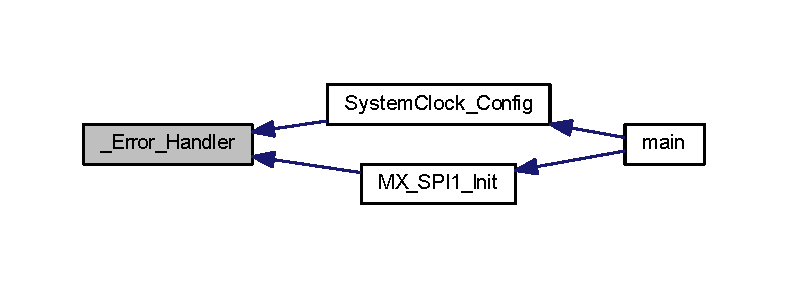
\includegraphics[width=350pt]{main_8c_a829116a51f1db1a72ebd1120f60719d5_icgraph}
\end{center}
\end{figure}
\mbox{\Hypertarget{main_8c_a840291bc02cba5474a4cb46a9b9566fe}\label{main_8c_a840291bc02cba5474a4cb46a9b9566fe}} 
\index{main.\+c@{main.\+c}!main@{main}}
\index{main@{main}!main.\+c@{main.\+c}}
\subsubsection{\texorpdfstring{main()}{main()}}
{\footnotesize\ttfamily int main (\begin{DoxyParamCaption}\item[{void}]{ }\end{DoxyParamCaption})}



That is Justing more un test about Doc application entry point. 


\begin{DoxyRetVals}{Return values}
{\em None} & \\
\hline
\end{DoxyRetVals}
\begin{DoxyWarning}{Warning}
T\+E\+ST Warning 
\end{DoxyWarning}


Definition at line 81 of file main.\+c.

Here is the call graph for this function\+:\nopagebreak
\begin{figure}[H]
\begin{center}
\leavevmode
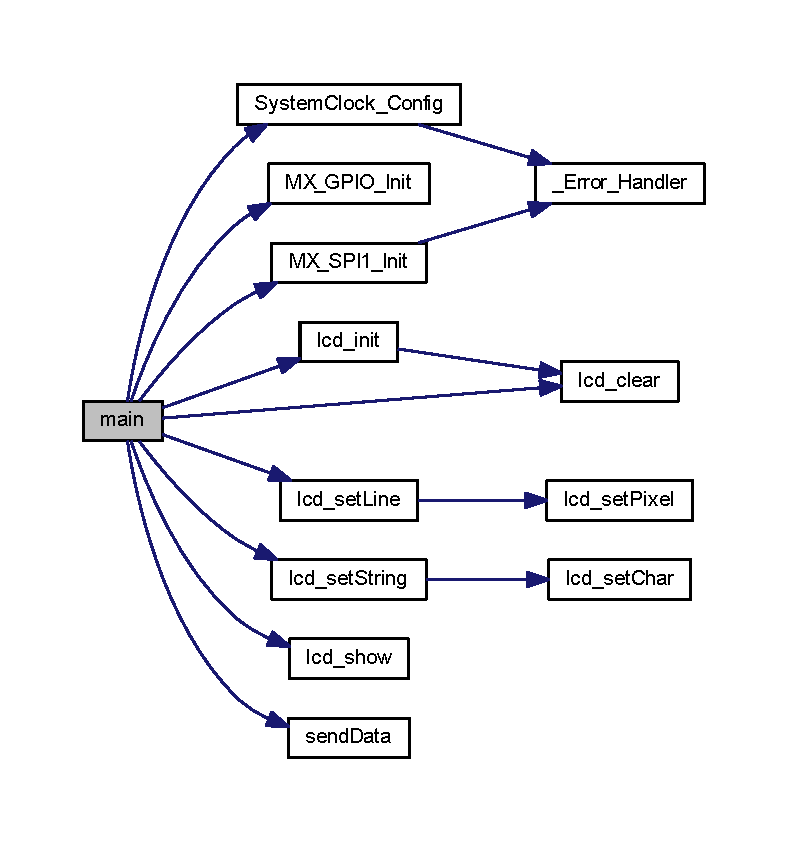
\includegraphics[width=350pt]{main_8c_a840291bc02cba5474a4cb46a9b9566fe_cgraph}
\end{center}
\end{figure}
\mbox{\Hypertarget{main_8c_a70af21c671abfcc773614a9a4f63d920}\label{main_8c_a70af21c671abfcc773614a9a4f63d920}} 
\index{main.\+c@{main.\+c}!System\+Clock\+\_\+\+Config@{System\+Clock\+\_\+\+Config}}
\index{System\+Clock\+\_\+\+Config@{System\+Clock\+\_\+\+Config}!main.\+c@{main.\+c}}
\subsubsection{\texorpdfstring{System\+Clock\+\_\+\+Config()}{SystemClock\_Config()}}
{\footnotesize\ttfamily void System\+Clock\+\_\+\+Config (\begin{DoxyParamCaption}\item[{void}]{ }\end{DoxyParamCaption})}



System Clock Configuration. 


\begin{DoxyRetVals}{Return values}
{\em None} & \\
\hline
\end{DoxyRetVals}
Configure the main internal regulator output voltage

Initializes the C\+PU, A\+HB and A\+PB busses clocks

Activate the Over-\/\+Drive mode

Initializes the C\+PU, A\+HB and A\+PB busses clocks

Configure the Systick interrupt time

Configure the Systick

Definition at line 138 of file main.\+c.

Here is the call graph for this function\+:\nopagebreak
\begin{figure}[H]
\begin{center}
\leavevmode
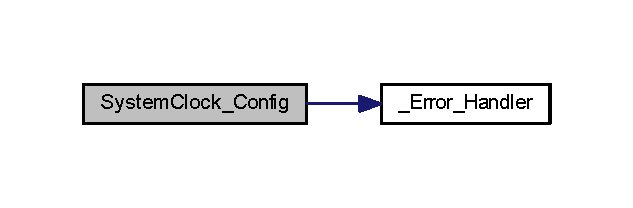
\includegraphics[width=304pt]{main_8c_a70af21c671abfcc773614a9a4f63d920_cgraph}
\end{center}
\end{figure}
Here is the caller graph for this function\+:
\nopagebreak
\begin{figure}[H]
\begin{center}
\leavevmode
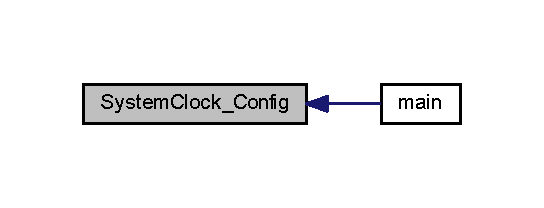
\includegraphics[width=261pt]{main_8c_a70af21c671abfcc773614a9a4f63d920_icgraph}
\end{center}
\end{figure}

\hypertarget{spi_8c}{}\section{Src/spi.c File Reference}
\label{spi_8c}\index{Src/spi.\+c@{Src/spi.\+c}}
{\ttfamily \#include \char`\"{}spi.\+h\char`\"{}}\newline
{\ttfamily \#include \char`\"{}gpio.\+h\char`\"{}}\newline
Include dependency graph for spi.\+c\+:\nopagebreak
\begin{figure}[H]
\begin{center}
\leavevmode
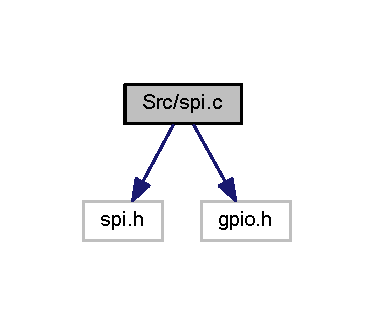
\includegraphics[width=180pt]{spi_8c__incl}
\end{center}
\end{figure}
\subsection*{Functions}
\begin{DoxyCompactItemize}
\item 
void \mbox{\hyperlink{spi_8c_af81398f9775695df0b172367651ca3e6}{M\+X\+\_\+\+S\+P\+I1\+\_\+\+Init}} (void)
\item 
void \mbox{\hyperlink{spi_8c_aea85daa666c03d85fd59edef711ebb08}{M\+X\+\_\+\+S\+P\+I2\+\_\+\+Init}} (void)
\item 
void \mbox{\hyperlink{spi_8c_a8e1dadd744299fa6f8bca0e1bcbd2c00}{H\+A\+L\+\_\+\+S\+P\+I\+\_\+\+Msp\+Init}} (S\+P\+I\+\_\+\+Handle\+Type\+Def $\ast$spi\+Handle)
\item 
void \mbox{\hyperlink{spi_8c_af9af6cae4cb9386b709196d3a3ab4f78}{H\+A\+L\+\_\+\+S\+P\+I\+\_\+\+Msp\+De\+Init}} (S\+P\+I\+\_\+\+Handle\+Type\+Def $\ast$spi\+Handle)
\end{DoxyCompactItemize}
\subsection*{Variables}
\begin{DoxyCompactItemize}
\item 
S\+P\+I\+\_\+\+Handle\+Type\+Def \mbox{\hyperlink{spi_8c_a9c6222bae4d0328dd843ae099623b40b}{hspi1}}
\item 
S\+P\+I\+\_\+\+Handle\+Type\+Def \mbox{\hyperlink{spi_8c_ab9da65f935e805137e2eb4e18c5ab224}{hspi2}}
\end{DoxyCompactItemize}


\subsection{Function Documentation}
\mbox{\Hypertarget{spi_8c_af9af6cae4cb9386b709196d3a3ab4f78}\label{spi_8c_af9af6cae4cb9386b709196d3a3ab4f78}} 
\index{spi.\+c@{spi.\+c}!H\+A\+L\+\_\+\+S\+P\+I\+\_\+\+Msp\+De\+Init@{H\+A\+L\+\_\+\+S\+P\+I\+\_\+\+Msp\+De\+Init}}
\index{H\+A\+L\+\_\+\+S\+P\+I\+\_\+\+Msp\+De\+Init@{H\+A\+L\+\_\+\+S\+P\+I\+\_\+\+Msp\+De\+Init}!spi.\+c@{spi.\+c}}
\subsubsection{\texorpdfstring{H\+A\+L\+\_\+\+S\+P\+I\+\_\+\+Msp\+De\+Init()}{HAL\_SPI\_MspDeInit()}}
{\footnotesize\ttfamily void H\+A\+L\+\_\+\+S\+P\+I\+\_\+\+Msp\+De\+Init (\begin{DoxyParamCaption}\item[{S\+P\+I\+\_\+\+Handle\+Type\+Def $\ast$}]{spi\+Handle }\end{DoxyParamCaption})}

S\+P\+I1 G\+P\+IO Configuration ~\newline
~\newline
P\+A5 ------$>$ S\+P\+I1\+\_\+\+S\+CK P\+A7 ------$>$ S\+P\+I1\+\_\+\+M\+O\+SI

S\+P\+I2 G\+P\+IO Configuration ~\newline
P\+B13 -\/-\/-\/---$>$ S\+P\+I2\+\_\+\+S\+CK P\+B14 -\/-\/-\/---$>$ S\+P\+I2\+\_\+\+M\+I\+SO P\+B15 -\/-\/-\/---$>$ S\+P\+I2\+\_\+\+M\+O\+SI

Definition at line 160 of file spi.\+c.

\mbox{\Hypertarget{spi_8c_a8e1dadd744299fa6f8bca0e1bcbd2c00}\label{spi_8c_a8e1dadd744299fa6f8bca0e1bcbd2c00}} 
\index{spi.\+c@{spi.\+c}!H\+A\+L\+\_\+\+S\+P\+I\+\_\+\+Msp\+Init@{H\+A\+L\+\_\+\+S\+P\+I\+\_\+\+Msp\+Init}}
\index{H\+A\+L\+\_\+\+S\+P\+I\+\_\+\+Msp\+Init@{H\+A\+L\+\_\+\+S\+P\+I\+\_\+\+Msp\+Init}!spi.\+c@{spi.\+c}}
\subsubsection{\texorpdfstring{H\+A\+L\+\_\+\+S\+P\+I\+\_\+\+Msp\+Init()}{HAL\_SPI\_MspInit()}}
{\footnotesize\ttfamily void H\+A\+L\+\_\+\+S\+P\+I\+\_\+\+Msp\+Init (\begin{DoxyParamCaption}\item[{S\+P\+I\+\_\+\+Handle\+Type\+Def $\ast$}]{spi\+Handle }\end{DoxyParamCaption})}

S\+P\+I1 G\+P\+IO Configuration ~\newline
~\newline
P\+A5 ------$>$ S\+P\+I1\+\_\+\+S\+CK P\+A7 ------$>$ S\+P\+I1\+\_\+\+M\+O\+SI

S\+P\+I2 G\+P\+IO Configuration ~\newline
P\+B13 -\/-\/-\/---$>$ S\+P\+I2\+\_\+\+S\+CK P\+B14 -\/-\/-\/---$>$ S\+P\+I2\+\_\+\+M\+I\+SO P\+B15 -\/-\/-\/---$>$ S\+P\+I2\+\_\+\+M\+O\+SI

Definition at line 107 of file spi.\+c.

\mbox{\Hypertarget{spi_8c_af81398f9775695df0b172367651ca3e6}\label{spi_8c_af81398f9775695df0b172367651ca3e6}} 
\index{spi.\+c@{spi.\+c}!M\+X\+\_\+\+S\+P\+I1\+\_\+\+Init@{M\+X\+\_\+\+S\+P\+I1\+\_\+\+Init}}
\index{M\+X\+\_\+\+S\+P\+I1\+\_\+\+Init@{M\+X\+\_\+\+S\+P\+I1\+\_\+\+Init}!spi.\+c@{spi.\+c}}
\subsubsection{\texorpdfstring{M\+X\+\_\+\+S\+P\+I1\+\_\+\+Init()}{MX\_SPI1\_Init()}}
{\footnotesize\ttfamily void M\+X\+\_\+\+S\+P\+I1\+\_\+\+Init (\begin{DoxyParamCaption}\item[{void}]{ }\end{DoxyParamCaption})}



Definition at line 63 of file spi.\+c.

Here is the call graph for this function\+:\nopagebreak
\begin{figure}[H]
\begin{center}
\leavevmode
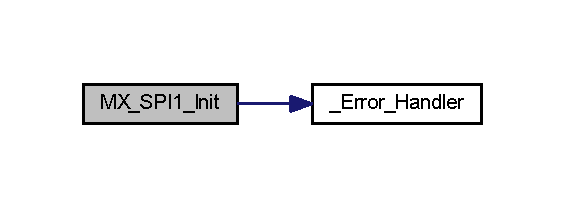
\includegraphics[width=271pt]{spi_8c_af81398f9775695df0b172367651ca3e6_cgraph}
\end{center}
\end{figure}
Here is the caller graph for this function\+:\nopagebreak
\begin{figure}[H]
\begin{center}
\leavevmode
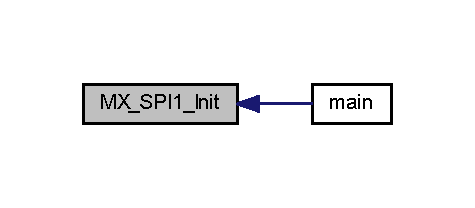
\includegraphics[width=312pt]{spi_8c_af81398f9775695df0b172367651ca3e6_icgraph}
\end{center}
\end{figure}
\mbox{\Hypertarget{spi_8c_aea85daa666c03d85fd59edef711ebb08}\label{spi_8c_aea85daa666c03d85fd59edef711ebb08}} 
\index{spi.\+c@{spi.\+c}!M\+X\+\_\+\+S\+P\+I2\+\_\+\+Init@{M\+X\+\_\+\+S\+P\+I2\+\_\+\+Init}}
\index{M\+X\+\_\+\+S\+P\+I2\+\_\+\+Init@{M\+X\+\_\+\+S\+P\+I2\+\_\+\+Init}!spi.\+c@{spi.\+c}}
\subsubsection{\texorpdfstring{M\+X\+\_\+\+S\+P\+I2\+\_\+\+Init()}{MX\_SPI2\_Init()}}
{\footnotesize\ttfamily void M\+X\+\_\+\+S\+P\+I2\+\_\+\+Init (\begin{DoxyParamCaption}\item[{void}]{ }\end{DoxyParamCaption})}



Definition at line 85 of file spi.\+c.

Here is the call graph for this function\+:\nopagebreak
\begin{figure}[H]
\begin{center}
\leavevmode
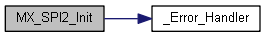
\includegraphics[width=271pt]{spi_8c_aea85daa666c03d85fd59edef711ebb08_cgraph}
\end{center}
\end{figure}
Here is the caller graph for this function\+:\nopagebreak
\begin{figure}[H]
\begin{center}
\leavevmode
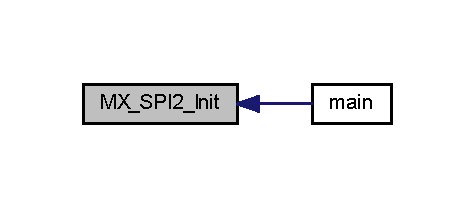
\includegraphics[width=228pt]{spi_8c_aea85daa666c03d85fd59edef711ebb08_icgraph}
\end{center}
\end{figure}


\subsection{Variable Documentation}
\mbox{\Hypertarget{spi_8c_a9c6222bae4d0328dd843ae099623b40b}\label{spi_8c_a9c6222bae4d0328dd843ae099623b40b}} 
\index{spi.\+c@{spi.\+c}!hspi1@{hspi1}}
\index{hspi1@{hspi1}!spi.\+c@{spi.\+c}}
\subsubsection{\texorpdfstring{hspi1}{hspi1}}
{\footnotesize\ttfamily S\+P\+I\+\_\+\+Handle\+Type\+Def hspi1}

File Name \+: \mbox{\hyperlink{spi_8c}{S\+P\+I.\+c}} Description \+: This file provides code for the configuration of the S\+PI instances.

This notice applies to any and all portions of this file that are not between comment pairs U\+S\+ER C\+O\+DE B\+E\+G\+IN and U\+S\+ER C\+O\+DE E\+ND. Other portions of this file, whether inserted by the user or by software development tools are owned by their respective copyright owners.

Copyright (c) 2018 S\+T\+Microelectronics International N.\+V. All rights reserved.

Redistribution and use in source and binary forms, with or without modification, are permitted, provided that the following conditions are met\+:


\begin{DoxyEnumerate}
\item Redistribution of source code must retain the above copyright notice, this list of conditions and the following disclaimer.
\item Redistributions in binary form must reproduce the above copyright notice, this list of conditions and the following disclaimer in the documentation and/or other materials provided with the distribution.
\item Neither the name of S\+T\+Microelectronics nor the names of other contributors to this software may be used to endorse or promote products derived from this software without specific written permission.
\item This software, including modifications and/or derivative works of this software, must execute solely and exclusively on microcontroller or microprocessor devices manufactured by or for S\+T\+Microelectronics.
\item Redistribution and use of this software other than as permitted under this license is void and will automatically terminate your rights under this license.
\end{DoxyEnumerate}

T\+H\+IS S\+O\+F\+T\+W\+A\+RE IS P\+R\+O\+V\+I\+D\+ED BY S\+T\+M\+I\+C\+R\+O\+E\+L\+E\+C\+T\+R\+O\+N\+I\+CS A\+ND C\+O\+N\+T\+R\+I\+B\+U\+T\+O\+RS \char`\"{}\+A\+S I\+S\char`\"{} A\+ND A\+NY E\+X\+P\+R\+E\+SS, I\+M\+P\+L\+I\+ED OR S\+T\+A\+T\+U\+T\+O\+RY W\+A\+R\+R\+A\+N\+T\+I\+ES, I\+N\+C\+L\+U\+D\+I\+NG, B\+UT N\+OT L\+I\+M\+I\+T\+ED TO, T\+HE I\+M\+P\+L\+I\+ED W\+A\+R\+R\+A\+N\+T\+I\+ES OF M\+E\+R\+C\+H\+A\+N\+T\+A\+B\+I\+L\+I\+TY, F\+I\+T\+N\+E\+SS F\+OR A P\+A\+R\+T\+I\+C\+U\+L\+AR P\+U\+R\+P\+O\+SE A\+ND N\+O\+N-\/\+I\+N\+F\+R\+I\+N\+G\+E\+M\+E\+NT OF T\+H\+I\+RD P\+A\+R\+TY I\+N\+T\+E\+L\+L\+E\+C\+T\+U\+AL P\+R\+O\+P\+E\+R\+TY R\+I\+G\+H\+TS A\+RE D\+I\+S\+C\+L\+A\+I\+M\+ED TO T\+HE F\+U\+L\+L\+E\+ST E\+X\+T\+E\+NT P\+E\+R\+M\+I\+T\+T\+ED BY L\+AW. IN NO E\+V\+E\+NT S\+H\+A\+LL S\+T\+M\+I\+C\+R\+O\+E\+L\+E\+C\+T\+R\+O\+N\+I\+CS OR C\+O\+N\+T\+R\+I\+B\+U\+T\+O\+RS BE L\+I\+A\+B\+LE F\+OR A\+NY D\+I\+R\+E\+CT, I\+N\+D\+I\+R\+E\+CT, I\+N\+C\+I\+D\+E\+N\+T\+AL, S\+P\+E\+C\+I\+AL, E\+X\+E\+M\+P\+L\+A\+RY, OR C\+O\+N\+S\+E\+Q\+U\+E\+N\+T\+I\+AL D\+A\+M\+A\+G\+ES (I\+N\+C\+L\+U\+D\+I\+NG, B\+UT N\+OT L\+I\+M\+I\+T\+ED TO, P\+R\+O\+C\+U\+R\+E\+M\+E\+NT OF S\+U\+B\+S\+T\+I\+T\+U\+TE G\+O\+O\+DS OR S\+E\+R\+V\+I\+C\+ES; L\+O\+SS OF U\+SE, D\+A\+TA, OR P\+R\+O\+F\+I\+TS; OR B\+U\+S\+I\+N\+E\+SS I\+N\+T\+E\+R\+R\+U\+P\+T\+I\+ON) H\+O\+W\+E\+V\+ER C\+A\+U\+S\+ED A\+ND ON A\+NY T\+H\+E\+O\+RY OF L\+I\+A\+B\+I\+L\+I\+TY, W\+H\+E\+T\+H\+ER IN C\+O\+N\+T\+R\+A\+CT, S\+T\+R\+I\+CT L\+I\+A\+B\+I\+L\+I\+TY, OR T\+O\+RT (I\+N\+C\+L\+U\+D\+I\+NG N\+E\+G\+L\+I\+G\+E\+N\+CE OR O\+T\+H\+E\+R\+W\+I\+SE) A\+R\+I\+S\+I\+NG IN A\+NY W\+AY O\+UT OF T\+HE U\+SE OF T\+H\+IS S\+O\+F\+T\+W\+A\+RE, E\+V\+EN IF A\+D\+V\+I\+S\+ED OF T\+HE P\+O\+S\+S\+I\+B\+I\+L\+I\+TY OF S\+U\+CH D\+A\+M\+A\+GE. 

Definition at line 59 of file spi.\+c.

\mbox{\Hypertarget{spi_8c_ab9da65f935e805137e2eb4e18c5ab224}\label{spi_8c_ab9da65f935e805137e2eb4e18c5ab224}} 
\index{spi.\+c@{spi.\+c}!hspi2@{hspi2}}
\index{hspi2@{hspi2}!spi.\+c@{spi.\+c}}
\subsubsection{\texorpdfstring{hspi2}{hspi2}}
{\footnotesize\ttfamily S\+P\+I\+\_\+\+Handle\+Type\+Def hspi2}



Definition at line 60 of file spi.\+c.


\hypertarget{stm32f4xx__hal__msp_8c}{}\section{stm32f4xx\+\_\+hal\+\_\+msp.\+c File Reference}
\label{stm32f4xx__hal__msp_8c}\index{stm32f4xx\+\_\+hal\+\_\+msp.\+c@{stm32f4xx\+\_\+hal\+\_\+msp.\+c}}
{\ttfamily \#include \char`\"{}stm32f4xx\+\_\+hal.\+h\char`\"{}}\newline
Include dependency graph for stm32f4xx\+\_\+hal\+\_\+msp.\+c\+:
\nopagebreak
\begin{figure}[H]
\begin{center}
\leavevmode
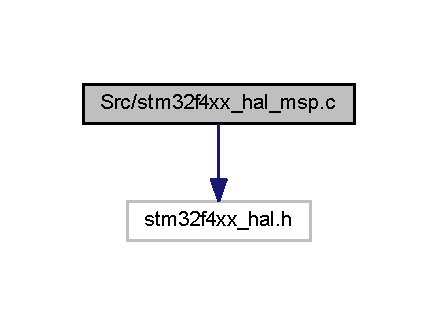
\includegraphics[width=192pt]{stm32f4xx__hal__msp_8c__incl}
\end{center}
\end{figure}
\subsection*{Functions}
\begin{DoxyCompactItemize}
\item 
void \mbox{\hyperlink{stm32f4xx__hal__msp_8c_a47642651029b93e3f9c9edad46bd27b4}{\+\_\+\+Error\+\_\+\+Handler}} (char $\ast$, int)
\begin{DoxyCompactList}\small\item\em This function is executed in case of error occurrence. \end{DoxyCompactList}\item 
void \mbox{\hyperlink{stm32f4xx__hal__msp_8c_ae4fb8e66865c87d0ebab74a726a6891f}{H\+A\+L\+\_\+\+Msp\+Init}} (void)
\end{DoxyCompactItemize}


\subsection{Function Documentation}
\mbox{\Hypertarget{stm32f4xx__hal__msp_8c_a47642651029b93e3f9c9edad46bd27b4}\label{stm32f4xx__hal__msp_8c_a47642651029b93e3f9c9edad46bd27b4}} 
\index{stm32f4xx\+\_\+hal\+\_\+msp.\+c@{stm32f4xx\+\_\+hal\+\_\+msp.\+c}!\+\_\+\+Error\+\_\+\+Handler@{\+\_\+\+Error\+\_\+\+Handler}}
\index{\+\_\+\+Error\+\_\+\+Handler@{\+\_\+\+Error\+\_\+\+Handler}!stm32f4xx\+\_\+hal\+\_\+msp.\+c@{stm32f4xx\+\_\+hal\+\_\+msp.\+c}}
\subsubsection{\texorpdfstring{\+\_\+\+Error\+\_\+\+Handler()}{\_Error\_Handler()}}
{\footnotesize\ttfamily void \+\_\+\+Error\+\_\+\+Handler (\begin{DoxyParamCaption}\item[{char $\ast$}]{file,  }\item[{int}]{line }\end{DoxyParamCaption})}



This function is executed in case of error occurrence. 

File Name \+: \mbox{\hyperlink{stm32f4xx__hal__msp_8c}{stm32f4xx\+\_\+hal\+\_\+msp.\+c}} Description \+: This file provides code for the M\+SP Initialization and de-\/\+Initialization codes.

This notice applies to any and all portions of this file that are not between comment pairs U\+S\+ER C\+O\+DE B\+E\+G\+IN and U\+S\+ER C\+O\+DE E\+ND. Other portions of this file, whether inserted by the user or by software development tools are owned by their respective copyright owners.

Copyright (c) 2018 S\+T\+Microelectronics International N.\+V. All rights reserved.

Redistribution and use in source and binary forms, with or without modification, are permitted, provided that the following conditions are met\+:


\begin{DoxyEnumerate}
\item Redistribution of source code must retain the above copyright notice, this list of conditions and the following disclaimer.
\item Redistributions in binary form must reproduce the above copyright notice, this list of conditions and the following disclaimer in the documentation and/or other materials provided with the distribution.
\item Neither the name of S\+T\+Microelectronics nor the names of other contributors to this software may be used to endorse or promote products derived from this software without specific written permission.
\item This software, including modifications and/or derivative works of this software, must execute solely and exclusively on microcontroller or microprocessor devices manufactured by or for S\+T\+Microelectronics.
\item Redistribution and use of this software other than as permitted under this license is void and will automatically terminate your rights under this license.
\end{DoxyEnumerate}

T\+H\+IS S\+O\+F\+T\+W\+A\+RE IS P\+R\+O\+V\+I\+D\+ED BY S\+T\+M\+I\+C\+R\+O\+E\+L\+E\+C\+T\+R\+O\+N\+I\+CS A\+ND C\+O\+N\+T\+R\+I\+B\+U\+T\+O\+RS \char`\"{}\+A\+S I\+S\char`\"{} A\+ND A\+NY E\+X\+P\+R\+E\+SS, I\+M\+P\+L\+I\+ED OR S\+T\+A\+T\+U\+T\+O\+RY W\+A\+R\+R\+A\+N\+T\+I\+ES, I\+N\+C\+L\+U\+D\+I\+NG, B\+UT N\+OT L\+I\+M\+I\+T\+ED TO, T\+HE I\+M\+P\+L\+I\+ED W\+A\+R\+R\+A\+N\+T\+I\+ES OF M\+E\+R\+C\+H\+A\+N\+T\+A\+B\+I\+L\+I\+TY, F\+I\+T\+N\+E\+SS F\+OR A P\+A\+R\+T\+I\+C\+U\+L\+AR P\+U\+R\+P\+O\+SE A\+ND N\+O\+N-\/\+I\+N\+F\+R\+I\+N\+G\+E\+M\+E\+NT OF T\+H\+I\+RD P\+A\+R\+TY I\+N\+T\+E\+L\+L\+E\+C\+T\+U\+AL P\+R\+O\+P\+E\+R\+TY R\+I\+G\+H\+TS A\+RE D\+I\+S\+C\+L\+A\+I\+M\+ED TO T\+HE F\+U\+L\+L\+E\+ST E\+X\+T\+E\+NT P\+E\+R\+M\+I\+T\+T\+ED BY L\+AW. IN NO E\+V\+E\+NT S\+H\+A\+LL S\+T\+M\+I\+C\+R\+O\+E\+L\+E\+C\+T\+R\+O\+N\+I\+CS OR C\+O\+N\+T\+R\+I\+B\+U\+T\+O\+RS BE L\+I\+A\+B\+LE F\+OR A\+NY D\+I\+R\+E\+CT, I\+N\+D\+I\+R\+E\+CT, I\+N\+C\+I\+D\+E\+N\+T\+AL, S\+P\+E\+C\+I\+AL, E\+X\+E\+M\+P\+L\+A\+RY, OR C\+O\+N\+S\+E\+Q\+U\+E\+N\+T\+I\+AL D\+A\+M\+A\+G\+ES (I\+N\+C\+L\+U\+D\+I\+NG, B\+UT N\+OT L\+I\+M\+I\+T\+ED TO, P\+R\+O\+C\+U\+R\+E\+M\+E\+NT OF S\+U\+B\+S\+T\+I\+T\+U\+TE G\+O\+O\+DS OR S\+E\+R\+V\+I\+C\+ES; L\+O\+SS OF U\+SE, D\+A\+TA, OR P\+R\+O\+F\+I\+TS; OR B\+U\+S\+I\+N\+E\+SS I\+N\+T\+E\+R\+R\+U\+P\+T\+I\+ON) H\+O\+W\+E\+V\+ER C\+A\+U\+S\+ED A\+ND ON A\+NY T\+H\+E\+O\+RY OF L\+I\+A\+B\+I\+L\+I\+TY, W\+H\+E\+T\+H\+ER IN C\+O\+N\+T\+R\+A\+CT, S\+T\+R\+I\+CT L\+I\+A\+B\+I\+L\+I\+TY, OR T\+O\+RT (I\+N\+C\+L\+U\+D\+I\+NG N\+E\+G\+L\+I\+G\+E\+N\+CE OR O\+T\+H\+E\+R\+W\+I\+SE) A\+R\+I\+S\+I\+NG IN A\+NY W\+AY O\+UT OF T\+HE U\+SE OF T\+H\+IS S\+O\+F\+T\+W\+A\+RE, E\+V\+EN IF A\+D\+V\+I\+S\+ED OF T\+HE P\+O\+S\+S\+I\+B\+I\+L\+I\+TY OF S\+U\+CH D\+A\+M\+A\+GE.


\begin{DoxyParams}{Parameters}
{\em file} & The file name as string. \\
\hline
{\em line} & The line in file as a number. \\
\hline
\end{DoxyParams}

\begin{DoxyRetVals}{Return values}
{\em None} & \\
\hline
\end{DoxyRetVals}


Definition at line 437 of file main.\+c.

Here is the caller graph for this function\+:
\nopagebreak
\begin{figure}[H]
\begin{center}
\leavevmode
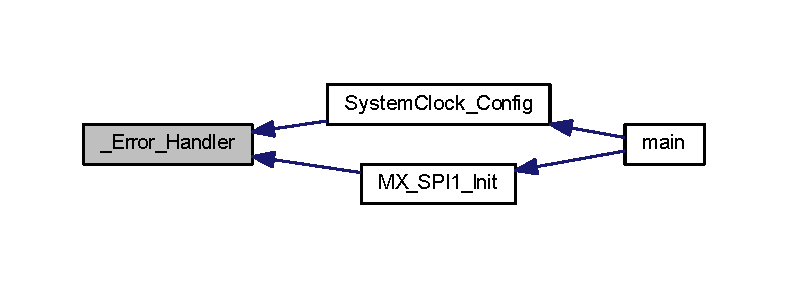
\includegraphics[width=350pt]{stm32f4xx__hal__msp_8c_a47642651029b93e3f9c9edad46bd27b4_icgraph}
\end{center}
\end{figure}
\mbox{\Hypertarget{stm32f4xx__hal__msp_8c_ae4fb8e66865c87d0ebab74a726a6891f}\label{stm32f4xx__hal__msp_8c_ae4fb8e66865c87d0ebab74a726a6891f}} 
\index{stm32f4xx\+\_\+hal\+\_\+msp.\+c@{stm32f4xx\+\_\+hal\+\_\+msp.\+c}!H\+A\+L\+\_\+\+Msp\+Init@{H\+A\+L\+\_\+\+Msp\+Init}}
\index{H\+A\+L\+\_\+\+Msp\+Init@{H\+A\+L\+\_\+\+Msp\+Init}!stm32f4xx\+\_\+hal\+\_\+msp.\+c@{stm32f4xx\+\_\+hal\+\_\+msp.\+c}}
\subsubsection{\texorpdfstring{H\+A\+L\+\_\+\+Msp\+Init()}{HAL\_MspInit()}}
{\footnotesize\ttfamily void H\+A\+L\+\_\+\+Msp\+Init (\begin{DoxyParamCaption}\item[{void}]{ }\end{DoxyParamCaption})}

Initializes the Global M\+SP. 

Definition at line 58 of file stm32f4xx\+\_\+hal\+\_\+msp.\+c.


\hypertarget{stm32f4xx__it_8c}{}\section{stm32f4xx\+\_\+it.\+c File Reference}
\label{stm32f4xx__it_8c}\index{stm32f4xx\+\_\+it.\+c@{stm32f4xx\+\_\+it.\+c}}


Interrupt Service Routines.  


{\ttfamily \#include \char`\"{}stm32f4xx\+\_\+hal.\+h\char`\"{}}\newline
{\ttfamily \#include \char`\"{}stm32f4xx.\+h\char`\"{}}\newline
{\ttfamily \#include \char`\"{}stm32f4xx\+\_\+it.\+h\char`\"{}}\newline
Include dependency graph for stm32f4xx\+\_\+it.\+c\+:
\nopagebreak
\begin{figure}[H]
\begin{center}
\leavevmode
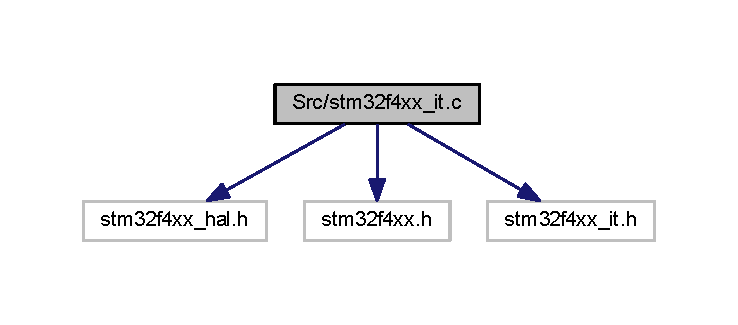
\includegraphics[width=350pt]{stm32f4xx__it_8c__incl}
\end{center}
\end{figure}
\subsection*{Functions}
\begin{DoxyCompactItemize}
\item 
void \mbox{\hyperlink{stm32f4xx__it_8c_a6ad7a5e3ee69cb6db6a6b9111ba898bc}{N\+M\+I\+\_\+\+Handler}} (void)
\begin{DoxyCompactList}\small\item\em This function handles Non maskable interrupt. \end{DoxyCompactList}\item 
void \mbox{\hyperlink{stm32f4xx__it_8c_a2bffc10d5bd4106753b7c30e86903bea}{Hard\+Fault\+\_\+\+Handler}} (void)
\begin{DoxyCompactList}\small\item\em This function handles Hard fault interrupt. \end{DoxyCompactList}\item 
void \mbox{\hyperlink{stm32f4xx__it_8c_a3150f74512510287a942624aa9b44cc5}{Mem\+Manage\+\_\+\+Handler}} (void)
\begin{DoxyCompactList}\small\item\em This function handles Memory management fault. \end{DoxyCompactList}\item 
void \mbox{\hyperlink{stm32f4xx__it_8c_a850cefb17a977292ae5eb4cafa9976c3}{Bus\+Fault\+\_\+\+Handler}} (void)
\begin{DoxyCompactList}\small\item\em This function handles Pre-\/fetch fault, memory access fault. \end{DoxyCompactList}\item 
void \mbox{\hyperlink{stm32f4xx__it_8c_a1d98923de2ed6b7309b66f9ba2971647}{Usage\+Fault\+\_\+\+Handler}} (void)
\begin{DoxyCompactList}\small\item\em This function handles Undefined instruction or illegal state. \end{DoxyCompactList}\item 
void \mbox{\hyperlink{stm32f4xx__it_8c_a3e5ddb3df0d62f2dc357e64a3f04a6ce}{S\+V\+C\+\_\+\+Handler}} (void)
\begin{DoxyCompactList}\small\item\em This function handles System service call via S\+WI instruction. \end{DoxyCompactList}\item 
void \mbox{\hyperlink{stm32f4xx__it_8c_adbdfb05858cc36fc520974df37ec3cb0}{Debug\+Mon\+\_\+\+Handler}} (void)
\begin{DoxyCompactList}\small\item\em This function handles Debug monitor. \end{DoxyCompactList}\item 
void \mbox{\hyperlink{stm32f4xx__it_8c_a6303e1f258cbdc1f970ce579cc015623}{Pend\+S\+V\+\_\+\+Handler}} (void)
\begin{DoxyCompactList}\small\item\em This function handles Pendable request for system service. \end{DoxyCompactList}\item 
void \mbox{\hyperlink{stm32f4xx__it_8c_ab5e09814056d617c521549e542639b7e}{Sys\+Tick\+\_\+\+Handler}} (void)
\begin{DoxyCompactList}\small\item\em This function handles System tick timer. \end{DoxyCompactList}\item 
void \mbox{\hyperlink{stm32f4xx__it_8c_ac201b60d58b0eba2ce0b55710eb3c4d0}{D\+M\+A1\+\_\+\+Stream5\+\_\+\+I\+R\+Q\+Handler}} (void)
\begin{DoxyCompactList}\small\item\em This function handles D\+M\+A1 stream5 global interrupt. \end{DoxyCompactList}\item 
void \mbox{\hyperlink{stm32f4xx__it_8c_aa28fd448462a6347589129f63bb0a388}{D\+M\+A1\+\_\+\+Stream6\+\_\+\+I\+R\+Q\+Handler}} (void)
\begin{DoxyCompactList}\small\item\em This function handles D\+M\+A1 stream6 global interrupt. \end{DoxyCompactList}\item 
void \mbox{\hyperlink{stm32f4xx__it_8c_a06406eadf297fa89a6eaf9586b227a69}{A\+D\+C\+\_\+\+I\+R\+Q\+Handler}} (void)
\begin{DoxyCompactList}\small\item\em This function handles A\+D\+C1, A\+D\+C2 and A\+D\+C3 interrupts. \end{DoxyCompactList}\item 
void \mbox{\hyperlink{stm32f4xx__it_8c_ac8e51d2183b5230cbd5481f8867adce9}{T\+I\+M3\+\_\+\+I\+R\+Q\+Handler}} (void)
\begin{DoxyCompactList}\small\item\em This function handles T\+I\+M3 global interrupt. \end{DoxyCompactList}\item 
void \mbox{\hyperlink{stm32f4xx__it_8c_a0ca6fd0e6f77921dd1123539857ba0a8}{U\+S\+A\+R\+T2\+\_\+\+I\+R\+Q\+Handler}} (void)
\begin{DoxyCompactList}\small\item\em This function handles U\+S\+A\+R\+T2 global interrupt. \end{DoxyCompactList}\item 
void \mbox{\hyperlink{stm32f4xx__it_8c_a5e66446caf21dd90191dc07a13ce2378}{T\+I\+M5\+\_\+\+I\+R\+Q\+Handler}} (void)
\begin{DoxyCompactList}\small\item\em This function handles T\+I\+M5 global interrupt. \end{DoxyCompactList}\end{DoxyCompactItemize}
\subsection*{Variables}
\begin{DoxyCompactItemize}
\item 
A\+D\+C\+\_\+\+Handle\+Type\+Def \mbox{\hyperlink{stm32f4xx__it_8c_a22b804736f5648d52f639b2647d4ed13}{hadc1}}
\item 
A\+D\+C\+\_\+\+Handle\+Type\+Def \mbox{\hyperlink{stm32f4xx__it_8c_acd9221f1aa19aebfe0b744947f2daf49}{hadc2}}
\item 
T\+I\+M\+\_\+\+Handle\+Type\+Def \mbox{\hyperlink{stm32f4xx__it_8c_aac3d2c59ee0e3bbae1b99529a154eb62}{htim3}}
\item 
T\+I\+M\+\_\+\+Handle\+Type\+Def \mbox{\hyperlink{stm32f4xx__it_8c_acefaeaaa3856ddddae7083b2d220fe4b}{htim5}}
\item 
D\+M\+A\+\_\+\+Handle\+Type\+Def \mbox{\hyperlink{stm32f4xx__it_8c_a0083b476c2a75ab9fb2ccbed0048857e}{hdma\+\_\+usart2\+\_\+tx}}
\item 
D\+M\+A\+\_\+\+Handle\+Type\+Def \mbox{\hyperlink{stm32f4xx__it_8c_a784aa25dc7e4580cfbf80658340f482c}{hdma\+\_\+usart2\+\_\+rx}}
\item 
U\+A\+R\+T\+\_\+\+Handle\+Type\+Def \mbox{\hyperlink{stm32f4xx__it_8c_aa9479c261d65eecedd3d9582f7f0f89c}{huart2}}
\end{DoxyCompactItemize}


\subsection{Detailed Description}
Interrupt Service Routines. 

C\+O\+P\+Y\+R\+I\+G\+H\+T(c) 2018 S\+T\+Microelectronics

Redistribution and use in source and binary forms, with or without modification, are permitted provided that the following conditions are met\+:
\begin{DoxyEnumerate}
\item Redistributions of source code must retain the above copyright notice, this list of conditions and the following disclaimer.
\item Redistributions in binary form must reproduce the above copyright notice, this list of conditions and the following disclaimer in the documentation and/or other materials provided with the distribution.
\item Neither the name of S\+T\+Microelectronics nor the names of its contributors may be used to endorse or promote products derived from this software without specific prior written permission.
\end{DoxyEnumerate}

T\+H\+IS S\+O\+F\+T\+W\+A\+RE IS P\+R\+O\+V\+I\+D\+ED BY T\+HE C\+O\+P\+Y\+R\+I\+G\+HT H\+O\+L\+D\+E\+RS A\+ND C\+O\+N\+T\+R\+I\+B\+U\+T\+O\+RS \char`\"{}\+A\+S I\+S\char`\"{} A\+ND A\+NY E\+X\+P\+R\+E\+SS OR I\+M\+P\+L\+I\+ED W\+A\+R\+R\+A\+N\+T\+I\+ES, I\+N\+C\+L\+U\+D\+I\+NG, B\+UT N\+OT L\+I\+M\+I\+T\+ED TO, T\+HE I\+M\+P\+L\+I\+ED W\+A\+R\+R\+A\+N\+T\+I\+ES OF M\+E\+R\+C\+H\+A\+N\+T\+A\+B\+I\+L\+I\+TY A\+ND F\+I\+T\+N\+E\+SS F\+OR A P\+A\+R\+T\+I\+C\+U\+L\+AR P\+U\+R\+P\+O\+SE A\+RE D\+I\+S\+C\+L\+A\+I\+M\+ED. IN NO E\+V\+E\+NT S\+H\+A\+LL T\+HE C\+O\+P\+Y\+R\+I\+G\+HT H\+O\+L\+D\+ER OR C\+O\+N\+T\+R\+I\+B\+U\+T\+O\+RS BE L\+I\+A\+B\+LE F\+OR A\+NY D\+I\+R\+E\+CT, I\+N\+D\+I\+R\+E\+CT, I\+N\+C\+I\+D\+E\+N\+T\+AL, S\+P\+E\+C\+I\+AL, E\+X\+E\+M\+P\+L\+A\+RY, OR C\+O\+N\+S\+E\+Q\+U\+E\+N\+T\+I\+AL D\+A\+M\+A\+G\+ES (I\+N\+C\+L\+U\+D\+I\+NG, B\+UT N\+OT L\+I\+M\+I\+T\+ED TO, P\+R\+O\+C\+U\+R\+E\+M\+E\+NT OF S\+U\+B\+S\+T\+I\+T\+U\+TE G\+O\+O\+DS OR S\+E\+R\+V\+I\+C\+ES; L\+O\+SS OF U\+SE, D\+A\+TA, OR P\+R\+O\+F\+I\+TS; OR B\+U\+S\+I\+N\+E\+SS I\+N\+T\+E\+R\+R\+U\+P\+T\+I\+ON) H\+O\+W\+E\+V\+ER C\+A\+U\+S\+ED A\+ND ON A\+NY T\+H\+E\+O\+RY OF L\+I\+A\+B\+I\+L\+I\+TY, W\+H\+E\+T\+H\+ER IN C\+O\+N\+T\+R\+A\+CT, S\+T\+R\+I\+CT L\+I\+A\+B\+I\+L\+I\+TY, OR T\+O\+RT (I\+N\+C\+L\+U\+D\+I\+NG N\+E\+G\+L\+I\+G\+E\+N\+CE OR O\+T\+H\+E\+R\+W\+I\+SE) A\+R\+I\+S\+I\+NG IN A\+NY W\+AY O\+UT OF T\+HE U\+SE OF T\+H\+IS S\+O\+F\+T\+W\+A\+RE, E\+V\+EN IF A\+D\+V\+I\+S\+ED OF T\+HE P\+O\+S\+S\+I\+B\+I\+L\+I\+TY OF S\+U\+CH D\+A\+M\+A\+GE. 

\subsection{Function Documentation}
\mbox{\Hypertarget{stm32f4xx__it_8c_a06406eadf297fa89a6eaf9586b227a69}\label{stm32f4xx__it_8c_a06406eadf297fa89a6eaf9586b227a69}} 
\index{stm32f4xx\+\_\+it.\+c@{stm32f4xx\+\_\+it.\+c}!A\+D\+C\+\_\+\+I\+R\+Q\+Handler@{A\+D\+C\+\_\+\+I\+R\+Q\+Handler}}
\index{A\+D\+C\+\_\+\+I\+R\+Q\+Handler@{A\+D\+C\+\_\+\+I\+R\+Q\+Handler}!stm32f4xx\+\_\+it.\+c@{stm32f4xx\+\_\+it.\+c}}
\subsubsection{\texorpdfstring{A\+D\+C\+\_\+\+I\+R\+Q\+Handler()}{ADC\_IRQHandler()}}
{\footnotesize\ttfamily void A\+D\+C\+\_\+\+I\+R\+Q\+Handler (\begin{DoxyParamCaption}\item[{void}]{ }\end{DoxyParamCaption})}



This function handles A\+D\+C1, A\+D\+C2 and A\+D\+C3 interrupts. 



Definition at line 232 of file stm32f4xx\+\_\+it.\+c.

\mbox{\Hypertarget{stm32f4xx__it_8c_a850cefb17a977292ae5eb4cafa9976c3}\label{stm32f4xx__it_8c_a850cefb17a977292ae5eb4cafa9976c3}} 
\index{stm32f4xx\+\_\+it.\+c@{stm32f4xx\+\_\+it.\+c}!Bus\+Fault\+\_\+\+Handler@{Bus\+Fault\+\_\+\+Handler}}
\index{Bus\+Fault\+\_\+\+Handler@{Bus\+Fault\+\_\+\+Handler}!stm32f4xx\+\_\+it.\+c@{stm32f4xx\+\_\+it.\+c}}
\subsubsection{\texorpdfstring{Bus\+Fault\+\_\+\+Handler()}{BusFault\_Handler()}}
{\footnotesize\ttfamily void Bus\+Fault\+\_\+\+Handler (\begin{DoxyParamCaption}\item[{void}]{ }\end{DoxyParamCaption})}



This function handles Pre-\/fetch fault, memory access fault. 



Definition at line 107 of file stm32f4xx\+\_\+it.\+c.

\mbox{\Hypertarget{stm32f4xx__it_8c_adbdfb05858cc36fc520974df37ec3cb0}\label{stm32f4xx__it_8c_adbdfb05858cc36fc520974df37ec3cb0}} 
\index{stm32f4xx\+\_\+it.\+c@{stm32f4xx\+\_\+it.\+c}!Debug\+Mon\+\_\+\+Handler@{Debug\+Mon\+\_\+\+Handler}}
\index{Debug\+Mon\+\_\+\+Handler@{Debug\+Mon\+\_\+\+Handler}!stm32f4xx\+\_\+it.\+c@{stm32f4xx\+\_\+it.\+c}}
\subsubsection{\texorpdfstring{Debug\+Mon\+\_\+\+Handler()}{DebugMon\_Handler()}}
{\footnotesize\ttfamily void Debug\+Mon\+\_\+\+Handler (\begin{DoxyParamCaption}\item[{void}]{ }\end{DoxyParamCaption})}



This function handles Debug monitor. 



Definition at line 156 of file stm32f4xx\+\_\+it.\+c.

\mbox{\Hypertarget{stm32f4xx__it_8c_ac201b60d58b0eba2ce0b55710eb3c4d0}\label{stm32f4xx__it_8c_ac201b60d58b0eba2ce0b55710eb3c4d0}} 
\index{stm32f4xx\+\_\+it.\+c@{stm32f4xx\+\_\+it.\+c}!D\+M\+A1\+\_\+\+Stream5\+\_\+\+I\+R\+Q\+Handler@{D\+M\+A1\+\_\+\+Stream5\+\_\+\+I\+R\+Q\+Handler}}
\index{D\+M\+A1\+\_\+\+Stream5\+\_\+\+I\+R\+Q\+Handler@{D\+M\+A1\+\_\+\+Stream5\+\_\+\+I\+R\+Q\+Handler}!stm32f4xx\+\_\+it.\+c@{stm32f4xx\+\_\+it.\+c}}
\subsubsection{\texorpdfstring{D\+M\+A1\+\_\+\+Stream5\+\_\+\+I\+R\+Q\+Handler()}{DMA1\_Stream5\_IRQHandler()}}
{\footnotesize\ttfamily void D\+M\+A1\+\_\+\+Stream5\+\_\+\+I\+R\+Q\+Handler (\begin{DoxyParamCaption}\item[{void}]{ }\end{DoxyParamCaption})}



This function handles D\+M\+A1 stream5 global interrupt. 



Definition at line 204 of file stm32f4xx\+\_\+it.\+c.

\mbox{\Hypertarget{stm32f4xx__it_8c_aa28fd448462a6347589129f63bb0a388}\label{stm32f4xx__it_8c_aa28fd448462a6347589129f63bb0a388}} 
\index{stm32f4xx\+\_\+it.\+c@{stm32f4xx\+\_\+it.\+c}!D\+M\+A1\+\_\+\+Stream6\+\_\+\+I\+R\+Q\+Handler@{D\+M\+A1\+\_\+\+Stream6\+\_\+\+I\+R\+Q\+Handler}}
\index{D\+M\+A1\+\_\+\+Stream6\+\_\+\+I\+R\+Q\+Handler@{D\+M\+A1\+\_\+\+Stream6\+\_\+\+I\+R\+Q\+Handler}!stm32f4xx\+\_\+it.\+c@{stm32f4xx\+\_\+it.\+c}}
\subsubsection{\texorpdfstring{D\+M\+A1\+\_\+\+Stream6\+\_\+\+I\+R\+Q\+Handler()}{DMA1\_Stream6\_IRQHandler()}}
{\footnotesize\ttfamily void D\+M\+A1\+\_\+\+Stream6\+\_\+\+I\+R\+Q\+Handler (\begin{DoxyParamCaption}\item[{void}]{ }\end{DoxyParamCaption})}



This function handles D\+M\+A1 stream6 global interrupt. 



Definition at line 218 of file stm32f4xx\+\_\+it.\+c.

\mbox{\Hypertarget{stm32f4xx__it_8c_a2bffc10d5bd4106753b7c30e86903bea}\label{stm32f4xx__it_8c_a2bffc10d5bd4106753b7c30e86903bea}} 
\index{stm32f4xx\+\_\+it.\+c@{stm32f4xx\+\_\+it.\+c}!Hard\+Fault\+\_\+\+Handler@{Hard\+Fault\+\_\+\+Handler}}
\index{Hard\+Fault\+\_\+\+Handler@{Hard\+Fault\+\_\+\+Handler}!stm32f4xx\+\_\+it.\+c@{stm32f4xx\+\_\+it.\+c}}
\subsubsection{\texorpdfstring{Hard\+Fault\+\_\+\+Handler()}{HardFault\_Handler()}}
{\footnotesize\ttfamily void Hard\+Fault\+\_\+\+Handler (\begin{DoxyParamCaption}\item[{void}]{ }\end{DoxyParamCaption})}



This function handles Hard fault interrupt. 



Definition at line 71 of file stm32f4xx\+\_\+it.\+c.

\mbox{\Hypertarget{stm32f4xx__it_8c_a3150f74512510287a942624aa9b44cc5}\label{stm32f4xx__it_8c_a3150f74512510287a942624aa9b44cc5}} 
\index{stm32f4xx\+\_\+it.\+c@{stm32f4xx\+\_\+it.\+c}!Mem\+Manage\+\_\+\+Handler@{Mem\+Manage\+\_\+\+Handler}}
\index{Mem\+Manage\+\_\+\+Handler@{Mem\+Manage\+\_\+\+Handler}!stm32f4xx\+\_\+it.\+c@{stm32f4xx\+\_\+it.\+c}}
\subsubsection{\texorpdfstring{Mem\+Manage\+\_\+\+Handler()}{MemManage\_Handler()}}
{\footnotesize\ttfamily void Mem\+Manage\+\_\+\+Handler (\begin{DoxyParamCaption}\item[{void}]{ }\end{DoxyParamCaption})}



This function handles Memory management fault. 



Definition at line 89 of file stm32f4xx\+\_\+it.\+c.

\mbox{\Hypertarget{stm32f4xx__it_8c_a6ad7a5e3ee69cb6db6a6b9111ba898bc}\label{stm32f4xx__it_8c_a6ad7a5e3ee69cb6db6a6b9111ba898bc}} 
\index{stm32f4xx\+\_\+it.\+c@{stm32f4xx\+\_\+it.\+c}!N\+M\+I\+\_\+\+Handler@{N\+M\+I\+\_\+\+Handler}}
\index{N\+M\+I\+\_\+\+Handler@{N\+M\+I\+\_\+\+Handler}!stm32f4xx\+\_\+it.\+c@{stm32f4xx\+\_\+it.\+c}}
\subsubsection{\texorpdfstring{N\+M\+I\+\_\+\+Handler()}{NMI\_Handler()}}
{\footnotesize\ttfamily void N\+M\+I\+\_\+\+Handler (\begin{DoxyParamCaption}\item[{void}]{ }\end{DoxyParamCaption})}



This function handles Non maskable interrupt. 



Definition at line 58 of file stm32f4xx\+\_\+it.\+c.

\mbox{\Hypertarget{stm32f4xx__it_8c_a6303e1f258cbdc1f970ce579cc015623}\label{stm32f4xx__it_8c_a6303e1f258cbdc1f970ce579cc015623}} 
\index{stm32f4xx\+\_\+it.\+c@{stm32f4xx\+\_\+it.\+c}!Pend\+S\+V\+\_\+\+Handler@{Pend\+S\+V\+\_\+\+Handler}}
\index{Pend\+S\+V\+\_\+\+Handler@{Pend\+S\+V\+\_\+\+Handler}!stm32f4xx\+\_\+it.\+c@{stm32f4xx\+\_\+it.\+c}}
\subsubsection{\texorpdfstring{Pend\+S\+V\+\_\+\+Handler()}{PendSV\_Handler()}}
{\footnotesize\ttfamily void Pend\+S\+V\+\_\+\+Handler (\begin{DoxyParamCaption}\item[{void}]{ }\end{DoxyParamCaption})}



This function handles Pendable request for system service. 



Definition at line 169 of file stm32f4xx\+\_\+it.\+c.

\mbox{\Hypertarget{stm32f4xx__it_8c_a3e5ddb3df0d62f2dc357e64a3f04a6ce}\label{stm32f4xx__it_8c_a3e5ddb3df0d62f2dc357e64a3f04a6ce}} 
\index{stm32f4xx\+\_\+it.\+c@{stm32f4xx\+\_\+it.\+c}!S\+V\+C\+\_\+\+Handler@{S\+V\+C\+\_\+\+Handler}}
\index{S\+V\+C\+\_\+\+Handler@{S\+V\+C\+\_\+\+Handler}!stm32f4xx\+\_\+it.\+c@{stm32f4xx\+\_\+it.\+c}}
\subsubsection{\texorpdfstring{S\+V\+C\+\_\+\+Handler()}{SVC\_Handler()}}
{\footnotesize\ttfamily void S\+V\+C\+\_\+\+Handler (\begin{DoxyParamCaption}\item[{void}]{ }\end{DoxyParamCaption})}



This function handles System service call via S\+WI instruction. 



Definition at line 143 of file stm32f4xx\+\_\+it.\+c.

\mbox{\Hypertarget{stm32f4xx__it_8c_ab5e09814056d617c521549e542639b7e}\label{stm32f4xx__it_8c_ab5e09814056d617c521549e542639b7e}} 
\index{stm32f4xx\+\_\+it.\+c@{stm32f4xx\+\_\+it.\+c}!Sys\+Tick\+\_\+\+Handler@{Sys\+Tick\+\_\+\+Handler}}
\index{Sys\+Tick\+\_\+\+Handler@{Sys\+Tick\+\_\+\+Handler}!stm32f4xx\+\_\+it.\+c@{stm32f4xx\+\_\+it.\+c}}
\subsubsection{\texorpdfstring{Sys\+Tick\+\_\+\+Handler()}{SysTick\_Handler()}}
{\footnotesize\ttfamily void Sys\+Tick\+\_\+\+Handler (\begin{DoxyParamCaption}\item[{void}]{ }\end{DoxyParamCaption})}



This function handles System tick timer. 



Definition at line 182 of file stm32f4xx\+\_\+it.\+c.

\mbox{\Hypertarget{stm32f4xx__it_8c_ac8e51d2183b5230cbd5481f8867adce9}\label{stm32f4xx__it_8c_ac8e51d2183b5230cbd5481f8867adce9}} 
\index{stm32f4xx\+\_\+it.\+c@{stm32f4xx\+\_\+it.\+c}!T\+I\+M3\+\_\+\+I\+R\+Q\+Handler@{T\+I\+M3\+\_\+\+I\+R\+Q\+Handler}}
\index{T\+I\+M3\+\_\+\+I\+R\+Q\+Handler@{T\+I\+M3\+\_\+\+I\+R\+Q\+Handler}!stm32f4xx\+\_\+it.\+c@{stm32f4xx\+\_\+it.\+c}}
\subsubsection{\texorpdfstring{T\+I\+M3\+\_\+\+I\+R\+Q\+Handler()}{TIM3\_IRQHandler()}}
{\footnotesize\ttfamily void T\+I\+M3\+\_\+\+I\+R\+Q\+Handler (\begin{DoxyParamCaption}\item[{void}]{ }\end{DoxyParamCaption})}



This function handles T\+I\+M3 global interrupt. 



Definition at line 247 of file stm32f4xx\+\_\+it.\+c.

\mbox{\Hypertarget{stm32f4xx__it_8c_a5e66446caf21dd90191dc07a13ce2378}\label{stm32f4xx__it_8c_a5e66446caf21dd90191dc07a13ce2378}} 
\index{stm32f4xx\+\_\+it.\+c@{stm32f4xx\+\_\+it.\+c}!T\+I\+M5\+\_\+\+I\+R\+Q\+Handler@{T\+I\+M5\+\_\+\+I\+R\+Q\+Handler}}
\index{T\+I\+M5\+\_\+\+I\+R\+Q\+Handler@{T\+I\+M5\+\_\+\+I\+R\+Q\+Handler}!stm32f4xx\+\_\+it.\+c@{stm32f4xx\+\_\+it.\+c}}
\subsubsection{\texorpdfstring{T\+I\+M5\+\_\+\+I\+R\+Q\+Handler()}{TIM5\_IRQHandler()}}
{\footnotesize\ttfamily void T\+I\+M5\+\_\+\+I\+R\+Q\+Handler (\begin{DoxyParamCaption}\item[{void}]{ }\end{DoxyParamCaption})}



This function handles T\+I\+M5 global interrupt. 



Definition at line 275 of file stm32f4xx\+\_\+it.\+c.

\mbox{\Hypertarget{stm32f4xx__it_8c_a1d98923de2ed6b7309b66f9ba2971647}\label{stm32f4xx__it_8c_a1d98923de2ed6b7309b66f9ba2971647}} 
\index{stm32f4xx\+\_\+it.\+c@{stm32f4xx\+\_\+it.\+c}!Usage\+Fault\+\_\+\+Handler@{Usage\+Fault\+\_\+\+Handler}}
\index{Usage\+Fault\+\_\+\+Handler@{Usage\+Fault\+\_\+\+Handler}!stm32f4xx\+\_\+it.\+c@{stm32f4xx\+\_\+it.\+c}}
\subsubsection{\texorpdfstring{Usage\+Fault\+\_\+\+Handler()}{UsageFault\_Handler()}}
{\footnotesize\ttfamily void Usage\+Fault\+\_\+\+Handler (\begin{DoxyParamCaption}\item[{void}]{ }\end{DoxyParamCaption})}



This function handles Undefined instruction or illegal state. 



Definition at line 125 of file stm32f4xx\+\_\+it.\+c.

\mbox{\Hypertarget{stm32f4xx__it_8c_a0ca6fd0e6f77921dd1123539857ba0a8}\label{stm32f4xx__it_8c_a0ca6fd0e6f77921dd1123539857ba0a8}} 
\index{stm32f4xx\+\_\+it.\+c@{stm32f4xx\+\_\+it.\+c}!U\+S\+A\+R\+T2\+\_\+\+I\+R\+Q\+Handler@{U\+S\+A\+R\+T2\+\_\+\+I\+R\+Q\+Handler}}
\index{U\+S\+A\+R\+T2\+\_\+\+I\+R\+Q\+Handler@{U\+S\+A\+R\+T2\+\_\+\+I\+R\+Q\+Handler}!stm32f4xx\+\_\+it.\+c@{stm32f4xx\+\_\+it.\+c}}
\subsubsection{\texorpdfstring{U\+S\+A\+R\+T2\+\_\+\+I\+R\+Q\+Handler()}{USART2\_IRQHandler()}}
{\footnotesize\ttfamily void U\+S\+A\+R\+T2\+\_\+\+I\+R\+Q\+Handler (\begin{DoxyParamCaption}\item[{void}]{ }\end{DoxyParamCaption})}



This function handles U\+S\+A\+R\+T2 global interrupt. 



Definition at line 261 of file stm32f4xx\+\_\+it.\+c.



\subsection{Variable Documentation}
\mbox{\Hypertarget{stm32f4xx__it_8c_a22b804736f5648d52f639b2647d4ed13}\label{stm32f4xx__it_8c_a22b804736f5648d52f639b2647d4ed13}} 
\index{stm32f4xx\+\_\+it.\+c@{stm32f4xx\+\_\+it.\+c}!hadc1@{hadc1}}
\index{hadc1@{hadc1}!stm32f4xx\+\_\+it.\+c@{stm32f4xx\+\_\+it.\+c}}
\subsubsection{\texorpdfstring{hadc1}{hadc1}}
{\footnotesize\ttfamily A\+D\+C\+\_\+\+Handle\+Type\+Def hadc1}

File Name \+: \mbox{\hyperlink{adc_8c}{A\+D\+C.\+c}} Description \+: This file provides code for the configuration of the A\+DC instances.

This notice applies to any and all portions of this file that are not between comment pairs U\+S\+ER C\+O\+DE B\+E\+G\+IN and U\+S\+ER C\+O\+DE E\+ND. Other portions of this file, whether inserted by the user or by software development tools are owned by their respective copyright owners.

Copyright (c) 2018 S\+T\+Microelectronics International N.\+V. All rights reserved.

Redistribution and use in source and binary forms, with or without modification, are permitted, provided that the following conditions are met\+:


\begin{DoxyEnumerate}
\item Redistribution of source code must retain the above copyright notice, this list of conditions and the following disclaimer.
\item Redistributions in binary form must reproduce the above copyright notice, this list of conditions and the following disclaimer in the documentation and/or other materials provided with the distribution.
\item Neither the name of S\+T\+Microelectronics nor the names of other contributors to this software may be used to endorse or promote products derived from this software without specific written permission.
\item This software, including modifications and/or derivative works of this software, must execute solely and exclusively on microcontroller or microprocessor devices manufactured by or for S\+T\+Microelectronics.
\item Redistribution and use of this software other than as permitted under this license is void and will automatically terminate your rights under this license.
\end{DoxyEnumerate}

T\+H\+IS S\+O\+F\+T\+W\+A\+RE IS P\+R\+O\+V\+I\+D\+ED BY S\+T\+M\+I\+C\+R\+O\+E\+L\+E\+C\+T\+R\+O\+N\+I\+CS A\+ND C\+O\+N\+T\+R\+I\+B\+U\+T\+O\+RS \char`\"{}\+A\+S I\+S\char`\"{} A\+ND A\+NY E\+X\+P\+R\+E\+SS, I\+M\+P\+L\+I\+ED OR S\+T\+A\+T\+U\+T\+O\+RY W\+A\+R\+R\+A\+N\+T\+I\+ES, I\+N\+C\+L\+U\+D\+I\+NG, B\+UT N\+OT L\+I\+M\+I\+T\+ED TO, T\+HE I\+M\+P\+L\+I\+ED W\+A\+R\+R\+A\+N\+T\+I\+ES OF M\+E\+R\+C\+H\+A\+N\+T\+A\+B\+I\+L\+I\+TY, F\+I\+T\+N\+E\+SS F\+OR A P\+A\+R\+T\+I\+C\+U\+L\+AR P\+U\+R\+P\+O\+SE A\+ND N\+O\+N-\/\+I\+N\+F\+R\+I\+N\+G\+E\+M\+E\+NT OF T\+H\+I\+RD P\+A\+R\+TY I\+N\+T\+E\+L\+L\+E\+C\+T\+U\+AL P\+R\+O\+P\+E\+R\+TY R\+I\+G\+H\+TS A\+RE D\+I\+S\+C\+L\+A\+I\+M\+ED TO T\+HE F\+U\+L\+L\+E\+ST E\+X\+T\+E\+NT P\+E\+R\+M\+I\+T\+T\+ED BY L\+AW. IN NO E\+V\+E\+NT S\+H\+A\+LL S\+T\+M\+I\+C\+R\+O\+E\+L\+E\+C\+T\+R\+O\+N\+I\+CS OR C\+O\+N\+T\+R\+I\+B\+U\+T\+O\+RS BE L\+I\+A\+B\+LE F\+OR A\+NY D\+I\+R\+E\+CT, I\+N\+D\+I\+R\+E\+CT, I\+N\+C\+I\+D\+E\+N\+T\+AL, S\+P\+E\+C\+I\+AL, E\+X\+E\+M\+P\+L\+A\+RY, OR C\+O\+N\+S\+E\+Q\+U\+E\+N\+T\+I\+AL D\+A\+M\+A\+G\+ES (I\+N\+C\+L\+U\+D\+I\+NG, B\+UT N\+OT L\+I\+M\+I\+T\+ED TO, P\+R\+O\+C\+U\+R\+E\+M\+E\+NT OF S\+U\+B\+S\+T\+I\+T\+U\+TE G\+O\+O\+DS OR S\+E\+R\+V\+I\+C\+ES; L\+O\+SS OF U\+SE, D\+A\+TA, OR P\+R\+O\+F\+I\+TS; OR B\+U\+S\+I\+N\+E\+SS I\+N\+T\+E\+R\+R\+U\+P\+T\+I\+ON) H\+O\+W\+E\+V\+ER C\+A\+U\+S\+ED A\+ND ON A\+NY T\+H\+E\+O\+RY OF L\+I\+A\+B\+I\+L\+I\+TY, W\+H\+E\+T\+H\+ER IN C\+O\+N\+T\+R\+A\+CT, S\+T\+R\+I\+CT L\+I\+A\+B\+I\+L\+I\+TY, OR T\+O\+RT (I\+N\+C\+L\+U\+D\+I\+NG N\+E\+G\+L\+I\+G\+E\+N\+CE OR O\+T\+H\+E\+R\+W\+I\+SE) A\+R\+I\+S\+I\+NG IN A\+NY W\+AY O\+UT OF T\+HE U\+SE OF T\+H\+IS S\+O\+F\+T\+W\+A\+RE, E\+V\+EN IF A\+D\+V\+I\+S\+ED OF T\+HE P\+O\+S\+S\+I\+B\+I\+L\+I\+TY OF S\+U\+CH D\+A\+M\+A\+GE. 

Definition at line 59 of file adc.\+c.

\mbox{\Hypertarget{stm32f4xx__it_8c_acd9221f1aa19aebfe0b744947f2daf49}\label{stm32f4xx__it_8c_acd9221f1aa19aebfe0b744947f2daf49}} 
\index{stm32f4xx\+\_\+it.\+c@{stm32f4xx\+\_\+it.\+c}!hadc2@{hadc2}}
\index{hadc2@{hadc2}!stm32f4xx\+\_\+it.\+c@{stm32f4xx\+\_\+it.\+c}}
\subsubsection{\texorpdfstring{hadc2}{hadc2}}
{\footnotesize\ttfamily A\+D\+C\+\_\+\+Handle\+Type\+Def hadc2}



Definition at line 60 of file adc.\+c.

\mbox{\Hypertarget{stm32f4xx__it_8c_a784aa25dc7e4580cfbf80658340f482c}\label{stm32f4xx__it_8c_a784aa25dc7e4580cfbf80658340f482c}} 
\index{stm32f4xx\+\_\+it.\+c@{stm32f4xx\+\_\+it.\+c}!hdma\+\_\+usart2\+\_\+rx@{hdma\+\_\+usart2\+\_\+rx}}
\index{hdma\+\_\+usart2\+\_\+rx@{hdma\+\_\+usart2\+\_\+rx}!stm32f4xx\+\_\+it.\+c@{stm32f4xx\+\_\+it.\+c}}
\subsubsection{\texorpdfstring{hdma\+\_\+usart2\+\_\+rx}{hdma\_usart2\_rx}}
{\footnotesize\ttfamily D\+M\+A\+\_\+\+Handle\+Type\+Def hdma\+\_\+usart2\+\_\+rx}



Definition at line 62 of file usart.\+c.

\mbox{\Hypertarget{stm32f4xx__it_8c_a0083b476c2a75ab9fb2ccbed0048857e}\label{stm32f4xx__it_8c_a0083b476c2a75ab9fb2ccbed0048857e}} 
\index{stm32f4xx\+\_\+it.\+c@{stm32f4xx\+\_\+it.\+c}!hdma\+\_\+usart2\+\_\+tx@{hdma\+\_\+usart2\+\_\+tx}}
\index{hdma\+\_\+usart2\+\_\+tx@{hdma\+\_\+usart2\+\_\+tx}!stm32f4xx\+\_\+it.\+c@{stm32f4xx\+\_\+it.\+c}}
\subsubsection{\texorpdfstring{hdma\+\_\+usart2\+\_\+tx}{hdma\_usart2\_tx}}
{\footnotesize\ttfamily D\+M\+A\+\_\+\+Handle\+Type\+Def hdma\+\_\+usart2\+\_\+tx}



Definition at line 61 of file usart.\+c.

\mbox{\Hypertarget{stm32f4xx__it_8c_aac3d2c59ee0e3bbae1b99529a154eb62}\label{stm32f4xx__it_8c_aac3d2c59ee0e3bbae1b99529a154eb62}} 
\index{stm32f4xx\+\_\+it.\+c@{stm32f4xx\+\_\+it.\+c}!htim3@{htim3}}
\index{htim3@{htim3}!stm32f4xx\+\_\+it.\+c@{stm32f4xx\+\_\+it.\+c}}
\subsubsection{\texorpdfstring{htim3}{htim3}}
{\footnotesize\ttfamily T\+I\+M\+\_\+\+Handle\+Type\+Def htim3}

File Name \+: \mbox{\hyperlink{tim_8c}{T\+I\+M.\+c}} Description \+: This file provides code for the configuration of the T\+IM instances.

This notice applies to any and all portions of this file that are not between comment pairs U\+S\+ER C\+O\+DE B\+E\+G\+IN and U\+S\+ER C\+O\+DE E\+ND. Other portions of this file, whether inserted by the user or by software development tools are owned by their respective copyright owners.

Copyright (c) 2018 S\+T\+Microelectronics International N.\+V. All rights reserved.

Redistribution and use in source and binary forms, with or without modification, are permitted, provided that the following conditions are met\+:


\begin{DoxyEnumerate}
\item Redistribution of source code must retain the above copyright notice, this list of conditions and the following disclaimer.
\item Redistributions in binary form must reproduce the above copyright notice, this list of conditions and the following disclaimer in the documentation and/or other materials provided with the distribution.
\item Neither the name of S\+T\+Microelectronics nor the names of other contributors to this software may be used to endorse or promote products derived from this software without specific written permission.
\item This software, including modifications and/or derivative works of this software, must execute solely and exclusively on microcontroller or microprocessor devices manufactured by or for S\+T\+Microelectronics.
\item Redistribution and use of this software other than as permitted under this license is void and will automatically terminate your rights under this license.
\end{DoxyEnumerate}

T\+H\+IS S\+O\+F\+T\+W\+A\+RE IS P\+R\+O\+V\+I\+D\+ED BY S\+T\+M\+I\+C\+R\+O\+E\+L\+E\+C\+T\+R\+O\+N\+I\+CS A\+ND C\+O\+N\+T\+R\+I\+B\+U\+T\+O\+RS \char`\"{}\+A\+S I\+S\char`\"{} A\+ND A\+NY E\+X\+P\+R\+E\+SS, I\+M\+P\+L\+I\+ED OR S\+T\+A\+T\+U\+T\+O\+RY W\+A\+R\+R\+A\+N\+T\+I\+ES, I\+N\+C\+L\+U\+D\+I\+NG, B\+UT N\+OT L\+I\+M\+I\+T\+ED TO, T\+HE I\+M\+P\+L\+I\+ED W\+A\+R\+R\+A\+N\+T\+I\+ES OF M\+E\+R\+C\+H\+A\+N\+T\+A\+B\+I\+L\+I\+TY, F\+I\+T\+N\+E\+SS F\+OR A P\+A\+R\+T\+I\+C\+U\+L\+AR P\+U\+R\+P\+O\+SE A\+ND N\+O\+N-\/\+I\+N\+F\+R\+I\+N\+G\+E\+M\+E\+NT OF T\+H\+I\+RD P\+A\+R\+TY I\+N\+T\+E\+L\+L\+E\+C\+T\+U\+AL P\+R\+O\+P\+E\+R\+TY R\+I\+G\+H\+TS A\+RE D\+I\+S\+C\+L\+A\+I\+M\+ED TO T\+HE F\+U\+L\+L\+E\+ST E\+X\+T\+E\+NT P\+E\+R\+M\+I\+T\+T\+ED BY L\+AW. IN NO E\+V\+E\+NT S\+H\+A\+LL S\+T\+M\+I\+C\+R\+O\+E\+L\+E\+C\+T\+R\+O\+N\+I\+CS OR C\+O\+N\+T\+R\+I\+B\+U\+T\+O\+RS BE L\+I\+A\+B\+LE F\+OR A\+NY D\+I\+R\+E\+CT, I\+N\+D\+I\+R\+E\+CT, I\+N\+C\+I\+D\+E\+N\+T\+AL, S\+P\+E\+C\+I\+AL, E\+X\+E\+M\+P\+L\+A\+RY, OR C\+O\+N\+S\+E\+Q\+U\+E\+N\+T\+I\+AL D\+A\+M\+A\+G\+ES (I\+N\+C\+L\+U\+D\+I\+NG, B\+UT N\+OT L\+I\+M\+I\+T\+ED TO, P\+R\+O\+C\+U\+R\+E\+M\+E\+NT OF S\+U\+B\+S\+T\+I\+T\+U\+TE G\+O\+O\+DS OR S\+E\+R\+V\+I\+C\+ES; L\+O\+SS OF U\+SE, D\+A\+TA, OR P\+R\+O\+F\+I\+TS; OR B\+U\+S\+I\+N\+E\+SS I\+N\+T\+E\+R\+R\+U\+P\+T\+I\+ON) H\+O\+W\+E\+V\+ER C\+A\+U\+S\+ED A\+ND ON A\+NY T\+H\+E\+O\+RY OF L\+I\+A\+B\+I\+L\+I\+TY, W\+H\+E\+T\+H\+ER IN C\+O\+N\+T\+R\+A\+CT, S\+T\+R\+I\+CT L\+I\+A\+B\+I\+L\+I\+TY, OR T\+O\+RT (I\+N\+C\+L\+U\+D\+I\+NG N\+E\+G\+L\+I\+G\+E\+N\+CE OR O\+T\+H\+E\+R\+W\+I\+SE) A\+R\+I\+S\+I\+NG IN A\+NY W\+AY O\+UT OF T\+HE U\+SE OF T\+H\+IS S\+O\+F\+T\+W\+A\+RE, E\+V\+EN IF A\+D\+V\+I\+S\+ED OF T\+HE P\+O\+S\+S\+I\+B\+I\+L\+I\+TY OF S\+U\+CH D\+A\+M\+A\+GE. 

Definition at line 57 of file tim.\+c.

\mbox{\Hypertarget{stm32f4xx__it_8c_acefaeaaa3856ddddae7083b2d220fe4b}\label{stm32f4xx__it_8c_acefaeaaa3856ddddae7083b2d220fe4b}} 
\index{stm32f4xx\+\_\+it.\+c@{stm32f4xx\+\_\+it.\+c}!htim5@{htim5}}
\index{htim5@{htim5}!stm32f4xx\+\_\+it.\+c@{stm32f4xx\+\_\+it.\+c}}
\subsubsection{\texorpdfstring{htim5}{htim5}}
{\footnotesize\ttfamily T\+I\+M\+\_\+\+Handle\+Type\+Def htim5}



Definition at line 58 of file tim.\+c.

\mbox{\Hypertarget{stm32f4xx__it_8c_aa9479c261d65eecedd3d9582f7f0f89c}\label{stm32f4xx__it_8c_aa9479c261d65eecedd3d9582f7f0f89c}} 
\index{stm32f4xx\+\_\+it.\+c@{stm32f4xx\+\_\+it.\+c}!huart2@{huart2}}
\index{huart2@{huart2}!stm32f4xx\+\_\+it.\+c@{stm32f4xx\+\_\+it.\+c}}
\subsubsection{\texorpdfstring{huart2}{huart2}}
{\footnotesize\ttfamily U\+A\+R\+T\+\_\+\+Handle\+Type\+Def huart2}

File Name \+: \mbox{\hyperlink{usart_8c}{U\+S\+A\+R\+T.\+c}} Description \+: This file provides code for the configuration of the U\+S\+A\+RT instances.

This notice applies to any and all portions of this file that are not between comment pairs U\+S\+ER C\+O\+DE B\+E\+G\+IN and U\+S\+ER C\+O\+DE E\+ND. Other portions of this file, whether inserted by the user or by software development tools are owned by their respective copyright owners.

Copyright (c) 2018 S\+T\+Microelectronics International N.\+V. All rights reserved.

Redistribution and use in source and binary forms, with or without modification, are permitted, provided that the following conditions are met\+:


\begin{DoxyEnumerate}
\item Redistribution of source code must retain the above copyright notice, this list of conditions and the following disclaimer.
\item Redistributions in binary form must reproduce the above copyright notice, this list of conditions and the following disclaimer in the documentation and/or other materials provided with the distribution.
\item Neither the name of S\+T\+Microelectronics nor the names of other contributors to this software may be used to endorse or promote products derived from this software without specific written permission.
\item This software, including modifications and/or derivative works of this software, must execute solely and exclusively on microcontroller or microprocessor devices manufactured by or for S\+T\+Microelectronics.
\item Redistribution and use of this software other than as permitted under this license is void and will automatically terminate your rights under this license.
\end{DoxyEnumerate}

T\+H\+IS S\+O\+F\+T\+W\+A\+RE IS P\+R\+O\+V\+I\+D\+ED BY S\+T\+M\+I\+C\+R\+O\+E\+L\+E\+C\+T\+R\+O\+N\+I\+CS A\+ND C\+O\+N\+T\+R\+I\+B\+U\+T\+O\+RS \char`\"{}\+A\+S I\+S\char`\"{} A\+ND A\+NY E\+X\+P\+R\+E\+SS, I\+M\+P\+L\+I\+ED OR S\+T\+A\+T\+U\+T\+O\+RY W\+A\+R\+R\+A\+N\+T\+I\+ES, I\+N\+C\+L\+U\+D\+I\+NG, B\+UT N\+OT L\+I\+M\+I\+T\+ED TO, T\+HE I\+M\+P\+L\+I\+ED W\+A\+R\+R\+A\+N\+T\+I\+ES OF M\+E\+R\+C\+H\+A\+N\+T\+A\+B\+I\+L\+I\+TY, F\+I\+T\+N\+E\+SS F\+OR A P\+A\+R\+T\+I\+C\+U\+L\+AR P\+U\+R\+P\+O\+SE A\+ND N\+O\+N-\/\+I\+N\+F\+R\+I\+N\+G\+E\+M\+E\+NT OF T\+H\+I\+RD P\+A\+R\+TY I\+N\+T\+E\+L\+L\+E\+C\+T\+U\+AL P\+R\+O\+P\+E\+R\+TY R\+I\+G\+H\+TS A\+RE D\+I\+S\+C\+L\+A\+I\+M\+ED TO T\+HE F\+U\+L\+L\+E\+ST E\+X\+T\+E\+NT P\+E\+R\+M\+I\+T\+T\+ED BY L\+AW. IN NO E\+V\+E\+NT S\+H\+A\+LL S\+T\+M\+I\+C\+R\+O\+E\+L\+E\+C\+T\+R\+O\+N\+I\+CS OR C\+O\+N\+T\+R\+I\+B\+U\+T\+O\+RS BE L\+I\+A\+B\+LE F\+OR A\+NY D\+I\+R\+E\+CT, I\+N\+D\+I\+R\+E\+CT, I\+N\+C\+I\+D\+E\+N\+T\+AL, S\+P\+E\+C\+I\+AL, E\+X\+E\+M\+P\+L\+A\+RY, OR C\+O\+N\+S\+E\+Q\+U\+E\+N\+T\+I\+AL D\+A\+M\+A\+G\+ES (I\+N\+C\+L\+U\+D\+I\+NG, B\+UT N\+OT L\+I\+M\+I\+T\+ED TO, P\+R\+O\+C\+U\+R\+E\+M\+E\+NT OF S\+U\+B\+S\+T\+I\+T\+U\+TE G\+O\+O\+DS OR S\+E\+R\+V\+I\+C\+ES; L\+O\+SS OF U\+SE, D\+A\+TA, OR P\+R\+O\+F\+I\+TS; OR B\+U\+S\+I\+N\+E\+SS I\+N\+T\+E\+R\+R\+U\+P\+T\+I\+ON) H\+O\+W\+E\+V\+ER C\+A\+U\+S\+ED A\+ND ON A\+NY T\+H\+E\+O\+RY OF L\+I\+A\+B\+I\+L\+I\+TY, W\+H\+E\+T\+H\+ER IN C\+O\+N\+T\+R\+A\+CT, S\+T\+R\+I\+CT L\+I\+A\+B\+I\+L\+I\+TY, OR T\+O\+RT (I\+N\+C\+L\+U\+D\+I\+NG N\+E\+G\+L\+I\+G\+E\+N\+CE OR O\+T\+H\+E\+R\+W\+I\+SE) A\+R\+I\+S\+I\+NG IN A\+NY W\+AY O\+UT OF T\+HE U\+SE OF T\+H\+IS S\+O\+F\+T\+W\+A\+RE, E\+V\+EN IF A\+D\+V\+I\+S\+ED OF T\+HE P\+O\+S\+S\+I\+B\+I\+L\+I\+TY OF S\+U\+CH D\+A\+M\+A\+GE. 

Definition at line 60 of file usart.\+c.


\hypertarget{system__stm32f4xx_8c}{}\section{system\+\_\+stm32f4xx.\+c File Reference}
\label{system__stm32f4xx_8c}\index{system\+\_\+stm32f4xx.\+c@{system\+\_\+stm32f4xx.\+c}}


C\+M\+S\+IS Cortex-\/\+M4 Device Peripheral Access Layer System Source File.  


{\ttfamily \#include \char`\"{}stm32f4xx.\+h\char`\"{}}\newline
Include dependency graph for system\+\_\+stm32f4xx.\+c\+:
\nopagebreak
\begin{figure}[H]
\begin{center}
\leavevmode
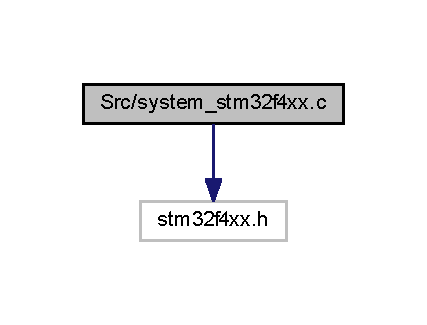
\includegraphics[width=187pt]{system__stm32f4xx_8c__incl}
\end{center}
\end{figure}
\subsection*{Macros}
\begin{DoxyCompactItemize}
\item 
\#define \mbox{\hyperlink{group___s_t_m32_f4xx___system___private___includes_gaeafcff4f57440c60e64812dddd13e7cb}{H\+S\+E\+\_\+\+V\+A\+L\+UE}}~((uint32\+\_\+t)25000000)
\item 
\#define \mbox{\hyperlink{group___s_t_m32_f4xx___system___private___includes_gaaa8c76e274d0f6dd2cefb5d0b17fbc37}{H\+S\+I\+\_\+\+V\+A\+L\+UE}}~((uint32\+\_\+t)16000000)
\item 
\#define \mbox{\hyperlink{group___s_t_m32_f4xx___system___private___defines_ga40e1495541cbb4acbe3f1819bd87a9fe}{V\+E\+C\+T\+\_\+\+T\+A\+B\+\_\+\+O\+F\+F\+S\+ET}}~0x00
\end{DoxyCompactItemize}
\subsection*{Functions}
\begin{DoxyCompactItemize}
\item 
void \mbox{\hyperlink{group___s_t_m32_f4xx___system___private___functions_ga93f514700ccf00d08dbdcff7f1224eb2}{System\+Init}} (void)
\begin{DoxyCompactList}\small\item\em Setup the microcontroller system Initialize the F\+PU setting, vector table location and External memory configuration. \end{DoxyCompactList}\item 
void \mbox{\hyperlink{group___s_t_m32_f4xx___system___private___functions_gae0c36a9591fe6e9c45ecb21a794f0f0f}{System\+Core\+Clock\+Update}} (void)
\begin{DoxyCompactList}\small\item\em Update System\+Core\+Clock variable according to Clock Register Values. The System\+Core\+Clock variable contains the core clock (H\+C\+LK), it can be used by the user application to setup the Sys\+Tick timer or configure other parameters. \end{DoxyCompactList}\end{DoxyCompactItemize}
\subsection*{Variables}
\begin{DoxyCompactItemize}
\item 
uint32\+\_\+t \mbox{\hyperlink{group___s_t_m32_f4xx___system___private___variables_gaa3cd3e43291e81e795d642b79b6088e6}{System\+Core\+Clock}} = 16000000
\item 
const uint8\+\_\+t \mbox{\hyperlink{group___s_t_m32_f4xx___system___private___variables_ga6e1d9cd666f0eacbfde31e9932a93466}{A\+H\+B\+Presc\+Table}} \mbox{[}16\mbox{]} = \{0, 0, 0, 0, 0, 0, 0, 0, 1, 2, 3, 4, 6, 7, 8, 9\}
\item 
const uint8\+\_\+t \mbox{\hyperlink{group___s_t_m32_f4xx___system___private___variables_ga5b4f8b768465842cf854a8f993b375e9}{A\+P\+B\+Presc\+Table}} \mbox{[}8\mbox{]} = \{0, 0, 0, 0, 1, 2, 3, 4\}
\end{DoxyCompactItemize}


\subsection{Detailed Description}
C\+M\+S\+IS Cortex-\/\+M4 Device Peripheral Access Layer System Source File. 

\begin{DoxyAuthor}{Author}
M\+CD Application Team This file provides two functions and one global variable to be called from user application\+:
\begin{DoxyItemize}
\item \mbox{\hyperlink{group___s_t_m32_f4xx___system___private___functions_ga93f514700ccf00d08dbdcff7f1224eb2}{System\+Init()}}\+: This function is called at startup just after reset and before branch to main program. This call is made inside the \char`\"{}startup\+\_\+stm32f4xx.\+s\char`\"{} file.
\item System\+Core\+Clock variable\+: Contains the core clock (H\+C\+LK), it can be used by the user application to setup the Sys\+Tick timer or configure other parameters.
\item \mbox{\hyperlink{group___s_t_m32_f4xx___system___private___functions_gae0c36a9591fe6e9c45ecb21a794f0f0f}{System\+Core\+Clock\+Update()}}\+: Updates the variable System\+Core\+Clock and must be called whenever the core clock is changed during program execution.
\end{DoxyItemize}
\end{DoxyAuthor}
\begin{DoxyAttention}{Attention}

\end{DoxyAttention}
\subsubsection*{\begin{center}\copyright{} C\+O\+P\+Y\+R\+I\+G\+HT 2017 S\+T\+Microelectronics\end{center} }

Redistribution and use in source and binary forms, with or without modification, are permitted provided that the following conditions are met\+:
\begin{DoxyEnumerate}
\item Redistributions of source code must retain the above copyright notice, this list of conditions and the following disclaimer.
\item Redistributions in binary form must reproduce the above copyright notice, this list of conditions and the following disclaimer in the documentation and/or other materials provided with the distribution.
\item Neither the name of S\+T\+Microelectronics nor the names of its contributors may be used to endorse or promote products derived from this software without specific prior written permission.
\end{DoxyEnumerate}

T\+H\+IS S\+O\+F\+T\+W\+A\+RE IS P\+R\+O\+V\+I\+D\+ED BY T\+HE C\+O\+P\+Y\+R\+I\+G\+HT H\+O\+L\+D\+E\+RS A\+ND C\+O\+N\+T\+R\+I\+B\+U\+T\+O\+RS \char`\"{}\+A\+S I\+S\char`\"{} A\+ND A\+NY E\+X\+P\+R\+E\+SS OR I\+M\+P\+L\+I\+ED W\+A\+R\+R\+A\+N\+T\+I\+ES, I\+N\+C\+L\+U\+D\+I\+NG, B\+UT N\+OT L\+I\+M\+I\+T\+ED TO, T\+HE I\+M\+P\+L\+I\+ED W\+A\+R\+R\+A\+N\+T\+I\+ES OF M\+E\+R\+C\+H\+A\+N\+T\+A\+B\+I\+L\+I\+TY A\+ND F\+I\+T\+N\+E\+SS F\+OR A P\+A\+R\+T\+I\+C\+U\+L\+AR P\+U\+R\+P\+O\+SE A\+RE D\+I\+S\+C\+L\+A\+I\+M\+ED. IN NO E\+V\+E\+NT S\+H\+A\+LL T\+HE C\+O\+P\+Y\+R\+I\+G\+HT H\+O\+L\+D\+ER OR C\+O\+N\+T\+R\+I\+B\+U\+T\+O\+RS BE L\+I\+A\+B\+LE F\+OR A\+NY D\+I\+R\+E\+CT, I\+N\+D\+I\+R\+E\+CT, I\+N\+C\+I\+D\+E\+N\+T\+AL, S\+P\+E\+C\+I\+AL, E\+X\+E\+M\+P\+L\+A\+RY, OR C\+O\+N\+S\+E\+Q\+U\+E\+N\+T\+I\+AL D\+A\+M\+A\+G\+ES (I\+N\+C\+L\+U\+D\+I\+NG, B\+UT N\+OT L\+I\+M\+I\+T\+ED TO, P\+R\+O\+C\+U\+R\+E\+M\+E\+NT OF S\+U\+B\+S\+T\+I\+T\+U\+TE G\+O\+O\+DS OR S\+E\+R\+V\+I\+C\+ES; L\+O\+SS OF U\+SE, D\+A\+TA, OR P\+R\+O\+F\+I\+TS; OR B\+U\+S\+I\+N\+E\+SS I\+N\+T\+E\+R\+R\+U\+P\+T\+I\+ON) H\+O\+W\+E\+V\+ER C\+A\+U\+S\+ED A\+ND ON A\+NY T\+H\+E\+O\+RY OF L\+I\+A\+B\+I\+L\+I\+TY, W\+H\+E\+T\+H\+ER IN C\+O\+N\+T\+R\+A\+CT, S\+T\+R\+I\+CT L\+I\+A\+B\+I\+L\+I\+TY, OR T\+O\+RT (I\+N\+C\+L\+U\+D\+I\+NG N\+E\+G\+L\+I\+G\+E\+N\+CE OR O\+T\+H\+E\+R\+W\+I\+SE) A\+R\+I\+S\+I\+NG IN A\+NY W\+AY O\+UT OF T\+HE U\+SE OF T\+H\+IS S\+O\+F\+T\+W\+A\+RE, E\+V\+EN IF A\+D\+V\+I\+S\+ED OF T\+HE P\+O\+S\+S\+I\+B\+I\+L\+I\+TY OF S\+U\+CH D\+A\+M\+A\+GE. 
\hypertarget{tmc260_8c}{}\section{Src/tmc260.c File Reference}
\label{tmc260_8c}\index{Src/tmc260.\+c@{Src/tmc260.\+c}}
{\ttfamily \#include \char`\"{}tmc260.\+h\char`\"{}}\newline
{\ttfamily \#include \char`\"{}tmc260\+\_\+driver.\+h\char`\"{}}\newline
Include dependency graph for tmc260.\+c\+:\nopagebreak
\begin{figure}[H]
\begin{center}
\leavevmode
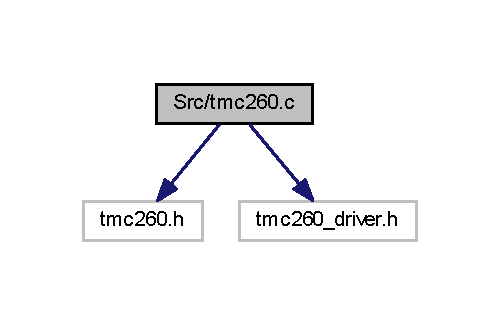
\includegraphics[width=240pt]{tmc260_8c__incl}
\end{center}
\end{figure}
\subsection*{Macros}
\begin{DoxyCompactItemize}
\item 
\#define \mbox{\hyperlink{tmc260_8c_acc9bef23a03bcb5ec9e9f6f23d3fd545}{I\+S\+\_\+\+I\+N\+\_\+\+P\+A\+R\+A\+M\+E\+T\+E\+R\+\_\+\+R\+A\+N\+GE}}(parameter,  value)~((value) $<$= tmc260\+\_\+parameter\+Maximum\+Raitings\mbox{[}(parameter)\mbox{]})
\item 
\#define \mbox{\hyperlink{tmc260_8c_a72a7769aca8f61958e2509bf5c8d6f2b}{I\+S\+\_\+\+V\+A\+L\+I\+D\+\_\+\+P\+A\+R\+A\+M\+E\+T\+ER}}(parameter)~((parameter)$>$=0 \&\& (parameter)$<$T\+M\+C260\+\_\+\+N\+U\+M\+B\+E\+R\+\_\+\+O\+F\+\_\+\+P\+A\+R\+A\+M\+E\+T\+E\+RS)
\item 
\#define \mbox{\hyperlink{tmc260_8c_aeaa59913a4ebfc9c21d1cc33bb114b2f}{T\+M\+C260\+\_\+\+R\+E\+G\+I\+S\+T\+E\+R\+\_\+\+N\+O\+T\+\_\+\+C\+H\+A\+N\+G\+ED}}~0
\item 
\#define \mbox{\hyperlink{tmc260_8c_ac5b755879478862fb105c52fd9639c19}{T\+M\+C260\+\_\+\+R\+E\+G\+I\+S\+T\+E\+R\+\_\+\+C\+H\+A\+N\+G\+ED}}~1
\end{DoxyCompactItemize}
\subsection*{Functions}
\begin{DoxyCompactItemize}
\item 
int8\+\_\+t \mbox{\hyperlink{tmc260_8c_a262a6cf5e8b10d0e07822d080b917ecc}{tmc260\+\_\+init}} (tmc260\+\_\+\+Device $\ast$const device)
\end{DoxyCompactItemize}


\subsection{Macro Definition Documentation}
\mbox{\Hypertarget{tmc260_8c_acc9bef23a03bcb5ec9e9f6f23d3fd545}\label{tmc260_8c_acc9bef23a03bcb5ec9e9f6f23d3fd545}} 
\index{tmc260.\+c@{tmc260.\+c}!I\+S\+\_\+\+I\+N\+\_\+\+P\+A\+R\+A\+M\+E\+T\+E\+R\+\_\+\+R\+A\+N\+GE@{I\+S\+\_\+\+I\+N\+\_\+\+P\+A\+R\+A\+M\+E\+T\+E\+R\+\_\+\+R\+A\+N\+GE}}
\index{I\+S\+\_\+\+I\+N\+\_\+\+P\+A\+R\+A\+M\+E\+T\+E\+R\+\_\+\+R\+A\+N\+GE@{I\+S\+\_\+\+I\+N\+\_\+\+P\+A\+R\+A\+M\+E\+T\+E\+R\+\_\+\+R\+A\+N\+GE}!tmc260.\+c@{tmc260.\+c}}
\subsubsection{\texorpdfstring{I\+S\+\_\+\+I\+N\+\_\+\+P\+A\+R\+A\+M\+E\+T\+E\+R\+\_\+\+R\+A\+N\+GE}{IS\_IN\_PARAMETER\_RANGE}}
{\footnotesize\ttfamily \#define I\+S\+\_\+\+I\+N\+\_\+\+P\+A\+R\+A\+M\+E\+T\+E\+R\+\_\+\+R\+A\+N\+GE(\begin{DoxyParamCaption}\item[{}]{parameter,  }\item[{}]{value }\end{DoxyParamCaption})~((value) $<$= tmc260\+\_\+parameter\+Maximum\+Raitings\mbox{[}(parameter)\mbox{]})}



Definition at line 6 of file tmc260.\+c.

\mbox{\Hypertarget{tmc260_8c_a72a7769aca8f61958e2509bf5c8d6f2b}\label{tmc260_8c_a72a7769aca8f61958e2509bf5c8d6f2b}} 
\index{tmc260.\+c@{tmc260.\+c}!I\+S\+\_\+\+V\+A\+L\+I\+D\+\_\+\+P\+A\+R\+A\+M\+E\+T\+ER@{I\+S\+\_\+\+V\+A\+L\+I\+D\+\_\+\+P\+A\+R\+A\+M\+E\+T\+ER}}
\index{I\+S\+\_\+\+V\+A\+L\+I\+D\+\_\+\+P\+A\+R\+A\+M\+E\+T\+ER@{I\+S\+\_\+\+V\+A\+L\+I\+D\+\_\+\+P\+A\+R\+A\+M\+E\+T\+ER}!tmc260.\+c@{tmc260.\+c}}
\subsubsection{\texorpdfstring{I\+S\+\_\+\+V\+A\+L\+I\+D\+\_\+\+P\+A\+R\+A\+M\+E\+T\+ER}{IS\_VALID\_PARAMETER}}
{\footnotesize\ttfamily \#define I\+S\+\_\+\+V\+A\+L\+I\+D\+\_\+\+P\+A\+R\+A\+M\+E\+T\+ER(\begin{DoxyParamCaption}\item[{}]{parameter }\end{DoxyParamCaption})~((parameter)$>$=0 \&\& (parameter)$<$T\+M\+C260\+\_\+\+N\+U\+M\+B\+E\+R\+\_\+\+O\+F\+\_\+\+P\+A\+R\+A\+M\+E\+T\+E\+RS)}



Definition at line 7 of file tmc260.\+c.

\mbox{\Hypertarget{tmc260_8c_ac5b755879478862fb105c52fd9639c19}\label{tmc260_8c_ac5b755879478862fb105c52fd9639c19}} 
\index{tmc260.\+c@{tmc260.\+c}!T\+M\+C260\+\_\+\+R\+E\+G\+I\+S\+T\+E\+R\+\_\+\+C\+H\+A\+N\+G\+ED@{T\+M\+C260\+\_\+\+R\+E\+G\+I\+S\+T\+E\+R\+\_\+\+C\+H\+A\+N\+G\+ED}}
\index{T\+M\+C260\+\_\+\+R\+E\+G\+I\+S\+T\+E\+R\+\_\+\+C\+H\+A\+N\+G\+ED@{T\+M\+C260\+\_\+\+R\+E\+G\+I\+S\+T\+E\+R\+\_\+\+C\+H\+A\+N\+G\+ED}!tmc260.\+c@{tmc260.\+c}}
\subsubsection{\texorpdfstring{T\+M\+C260\+\_\+\+R\+E\+G\+I\+S\+T\+E\+R\+\_\+\+C\+H\+A\+N\+G\+ED}{TMC260\_REGISTER\_CHANGED}}
{\footnotesize\ttfamily \#define T\+M\+C260\+\_\+\+R\+E\+G\+I\+S\+T\+E\+R\+\_\+\+C\+H\+A\+N\+G\+ED~1}



Definition at line 11 of file tmc260.\+c.

\mbox{\Hypertarget{tmc260_8c_aeaa59913a4ebfc9c21d1cc33bb114b2f}\label{tmc260_8c_aeaa59913a4ebfc9c21d1cc33bb114b2f}} 
\index{tmc260.\+c@{tmc260.\+c}!T\+M\+C260\+\_\+\+R\+E\+G\+I\+S\+T\+E\+R\+\_\+\+N\+O\+T\+\_\+\+C\+H\+A\+N\+G\+ED@{T\+M\+C260\+\_\+\+R\+E\+G\+I\+S\+T\+E\+R\+\_\+\+N\+O\+T\+\_\+\+C\+H\+A\+N\+G\+ED}}
\index{T\+M\+C260\+\_\+\+R\+E\+G\+I\+S\+T\+E\+R\+\_\+\+N\+O\+T\+\_\+\+C\+H\+A\+N\+G\+ED@{T\+M\+C260\+\_\+\+R\+E\+G\+I\+S\+T\+E\+R\+\_\+\+N\+O\+T\+\_\+\+C\+H\+A\+N\+G\+ED}!tmc260.\+c@{tmc260.\+c}}
\subsubsection{\texorpdfstring{T\+M\+C260\+\_\+\+R\+E\+G\+I\+S\+T\+E\+R\+\_\+\+N\+O\+T\+\_\+\+C\+H\+A\+N\+G\+ED}{TMC260\_REGISTER\_NOT\_CHANGED}}
{\footnotesize\ttfamily \#define T\+M\+C260\+\_\+\+R\+E\+G\+I\+S\+T\+E\+R\+\_\+\+N\+O\+T\+\_\+\+C\+H\+A\+N\+G\+ED~0}



Definition at line 10 of file tmc260.\+c.



\subsection{Function Documentation}
\mbox{\Hypertarget{tmc260_8c_a262a6cf5e8b10d0e07822d080b917ecc}\label{tmc260_8c_a262a6cf5e8b10d0e07822d080b917ecc}} 
\index{tmc260.\+c@{tmc260.\+c}!tmc260\+\_\+init@{tmc260\+\_\+init}}
\index{tmc260\+\_\+init@{tmc260\+\_\+init}!tmc260.\+c@{tmc260.\+c}}
\subsubsection{\texorpdfstring{tmc260\+\_\+init()}{tmc260\_init()}}
{\footnotesize\ttfamily int8\+\_\+t tmc260\+\_\+init (\begin{DoxyParamCaption}\item[{tmc260\+\_\+\+Device $\ast$const}]{device }\end{DoxyParamCaption})}



Definition at line 54 of file tmc260.\+c.


\hypertarget{tmc260__driver_8c}{}\section{Src/tmc260\+\_\+driver.c File Reference}
\label{tmc260__driver_8c}\index{Src/tmc260\+\_\+driver.\+c@{Src/tmc260\+\_\+driver.\+c}}
{\ttfamily \#include \char`\"{}tmc260\+\_\+driver.\+h\char`\"{}}\newline
Include dependency graph for tmc260\+\_\+driver.\+c\+:\nopagebreak
\begin{figure}[H]
\begin{center}
\leavevmode
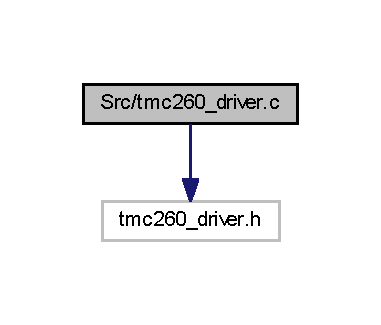
\includegraphics[width=183pt]{tmc260__driver_8c__incl}
\end{center}
\end{figure}
\subsection*{Functions}
\begin{DoxyCompactItemize}
\item 
int8\+\_\+t \mbox{\hyperlink{tmc260__driver_8c_a41285d5564a6dd86fee6bd203f3fbfc0}{tmc260\+\_\+\+Registers\+\_\+init}} (tmc260\+\_\+\+Register\+Set $\ast$device)
\end{DoxyCompactItemize}


\subsection{Function Documentation}
\mbox{\Hypertarget{tmc260__driver_8c_a41285d5564a6dd86fee6bd203f3fbfc0}\label{tmc260__driver_8c_a41285d5564a6dd86fee6bd203f3fbfc0}} 
\index{tmc260\+\_\+driver.\+c@{tmc260\+\_\+driver.\+c}!tmc260\+\_\+\+Registers\+\_\+init@{tmc260\+\_\+\+Registers\+\_\+init}}
\index{tmc260\+\_\+\+Registers\+\_\+init@{tmc260\+\_\+\+Registers\+\_\+init}!tmc260\+\_\+driver.\+c@{tmc260\+\_\+driver.\+c}}
\subsubsection{\texorpdfstring{tmc260\+\_\+\+Registers\+\_\+init()}{tmc260\_Registers\_init()}}
{\footnotesize\ttfamily int8\+\_\+t tmc260\+\_\+\+Registers\+\_\+init (\begin{DoxyParamCaption}\item[{tmc260\+\_\+\+Register\+Set $\ast$}]{device }\end{DoxyParamCaption})}



Definition at line 93 of file tmc260\+\_\+driver.\+c.


%--- End generated contents ---

% Index
\backmatter
\newpage
\phantomsection
\clearemptydoublepage
\addcontentsline{toc}{chapter}{Index}
\printindex

\end{document}
